% !TEX program = pdflatex
% !BIB program = biber

% !TEX program = pdflatex
% !BIB program = biber

% !TEX root = main.tex
\documentclass[10pt, a4paper]{article}
% \documentclass[12pt, a4paper, oneside]{memoir}
% \chapterstyle{veelo}

%% Sets page size and margins
\usepackage[a4paper,top=3cm,bottom=2cm,left=3cm,right=3cm,marginparwidth=1.75cm]{geometry}
%\usepackage[left=2cm,top=2cm,bottom=2cm,bindingoffset=1cm]{geometry}

\usepackage[utf8x]{inputenc}
\usepackage{graphicx}
\usepackage{float}
\usepackage{imakeidx}
\usepackage{amsmath}
\usepackage[colorlinks=true, allcolors=blue]{hyperref}
\usepackage{graphicx}
\usepackage{float}
\usepackage{imakeidx}
\usepackage{amsmath}
\usepackage{url}
\usepackage[export]{adjustbox}
\usepackage{subcaption}
\usepackage{booktabs}
\usepackage{pdflscape}
\usepackage[table,xcdraw]{xcolor}
%\usepackage{svg}

%% Useful packages
\usepackage[colorinlistoftodos]{todonotes}
\usepackage[T1]{fontenc}

%% Language and font encodings
\usepackage[english]{babel}

%% Define a few colours to be used throughout the document
\usepackage{tikz,xcolor}
\definecolor{TextColor}{HTML}{000000}
\definecolor{SideColorDark}{HTML}{000000}
\definecolor{MainColor}{HTML}{0000FF}
\definecolor{OppositeColor}{HTML}{FF0000}
\definecolor{HighlightColor}{HTML}{FFFF00}


%% Code block style
%  Load the \ttfamily font
\usepackage[T1]{fontenc}
\usepackage[scaled]{beramono}

%  Format code blocks
\usepackage{listings}
%  Change caption name
\renewcommand*{\lstlistingname}{Code block}
\captionsetup[lstlisting]{margin=0cm,format=hang,font=small,format=plain,labelfont={bf,up},textfont={it}}
%  Style
\lstset{
  showstringspaces=false,
  formfeed=\newpage,
  commentstyle=\itshape,
  backgroundcolor=\color{gray!5},
  breakatwhitespace=false,         % sets if automatic breaks should only happen at whitespace
  breaklines=true,                 % sets automatic line breaking
  captionpos=b,                    % sets the caption-position to bottom
  commentstyle=\color{gray},    % comment style
  escapeinside={\%*}{*)},          % if you want to add LaTeX within your code
  keepspaces=true,
  numbersep=2mm,                   % how far the line-numbers are from the code
  showspaces=false,
  showstringspaces=false,
  showtabs=false,
  stepnumber=1, numberfirstline=false,
  basicstyle=\linespread{1}\footnotesize\ttfamily,
  keywordstyle=\bfseries\color{MainColor},
  stringstyle=\itshape\color{OppositeColor},
  numberstyle=\footnotesize\ttfamily\color{gray},
  numbers=left,xleftmargin=4mm,framexleftmargin=0mm,xrightmargin=0mm,
  frame=top,frame=bottom,
}

\title{Project Management\\Assignment 1}
\author{Daniel Robinson\\18361137}

\pagenumbering{roman}

\begin{document}
% \maketitle
    \begin{titlepage}
        \begin{center}
            \vspace*{1cm}
            
            \begin{figure}
			\centering
            
\includegraphics[scale=2]{UScrest-top.jpg}
            \end{figure}
            
            \huge
            \textbf{Project Management 412\\Assignment 1\\Team G2}
            
            \vspace{1.5cm}
            
            \large
            Peter Toulouras\\
            18296831\\
            \vspace{0.5cm}
            Biance Huysamen\\
            18200648\\
            \vspace{0.5cm}
            Carmen Steyn\\
            18183093\\
            \vspace{0.5cm}
            Eduard van der Merwe\\
            18214746\\
            \vspace{0.5cm}
            Sarel Swart\\
            17508150\\
            \vspace{0.5cm}
            Daniel Robinson\\
            18361137\\
            \vspace{3.5cm}
            
            \large
            Date: 28 February 2017
            
        \end{center}
\end{titlepage}

\newpage

% \begin{abstract}
% Your abstract.
% \end{abstract}


\section*{Plagiarism Declaration}

I know that plagiarism is wrong.\\\\
\noindent
Plagiarism is to use another's work (even if it is summarised, translated or rephrased) and pretend that it is one's own. This assignment is our own work.\\\\
\noindent
Each contribution to and quotation (e.g. "cut and paste") in this assignment from the work(s) of other people has been explicitly attributed, and has been cited and referenced. In addition to being explicitly attributed, all quotations are enclosed in inverted commas, and long quotations are additionally in indented paragraphs.\\\\
\noindent
I have not allowed, and will not allow, anyone to use my work (in paper, graphics, electronic, verbal or any other format) with the intention of passing it off as his/her own work.\\\\
\noindent
I know that a mark of zero may be awarded to assignments with plagiarism and also that no opportunity be given to submit an improved assignment.\\\\
\noindent
I know that students involved in plagiarism will be reported to the Registrar and/or the Central Disciplinary Committee.

\section*{Executive Summary}
In today's day and age, engineers are expected to be versatile in more aspects than ever
before. One of these is project management. This assignment hopes to introduce and
ready engineering students for project management and as close to reality as possible. For
example, the teams of students are multi-disciplinary, and had most probably not had prior
experience working together. For this particular assignment, a project structure has been designed in order to manage the creation of a beer brewery.\\

\noindent
Throughout this document the team will be working to create the product in a 11 month period with a budget of \$380 000. The students need to use these restrictions and plan how they will use the resources to complete the project. The resources will be bid on by using a simulation program called Sim4Projects. Using this program, the students have to bid against other teams to create a real life simulation. To bid on these resources they need to determine how much they are willing to spend on the different resources and how much they will be willing to spend on training these resources. By creating a budget that corresponds with the baseline plan they can determine how they can manage the resources.\\

\noindent
To manage the resources, the team needs to identify the objectives of the project as part of the project scope. If the objectives are determined they can then create deliverables so that he project stays on track and on budget. Milestones are put together and the critical tasks will be identified. The milestones also help insure that the project will stay within the time frame. A work breakdown structure will also be structured to help insure that project will stay on schedule. By doing this the work can then be divided between the different engineers to ensure the skills of all the engineers are used optimally. Project requirements, limitations and exclusions must be identified so that it is clear what is possible and what is not possible during the process of creating the brewery. The last part of the project scope is to review and approve all the decisions made so that the process of creating the project can begin.
\\

\noindent
Using Microsoft Project, the students can create a baseline plan that will give a visual aid to determine if the project is on track with the estimated times. By putting more people on certain project they can then reduce the time that the project will and ensure that the project will be finished within the set time frame. Using this baseline, they can then setup an estimated budget.\\

\noindent
The budget that is created is setup for a perfect scenario were everything runs smoothly and without any interruptions. In real life this will not always be the situation. In some circumstances there will be risks involved that may change the timeline and the budget of the project. The team need to be prepared for these situations. Risks need to be identified and analysed. A Risk Assessment Plan is set up to evaluate the risk and how these risks will be managed. 


\newpage
\tableofcontents
\listoffigures
\listoftables

\newpage
\section{Introduction}

\pagenumbering{arabic}

Stellenbosch is a beautiful town surrounded by magnificent wine lands and farms.  However this town is in need of a beer brewery that will cater for the vibrant student life of Stellenbosch.\\

\noindent
The well-know Stellenbrau company is interested in starting a local micro-brewery in the heart of Stellenbosch combined with a restaurant.\\

\noindent
Using a multi-disciplinary group every member can contribute in a way to insures that an optimal solution can be found. This multi-disciplinary will consist out of an Electrical engineer, a civil engineer, a mechanical engineer, a chemical engineer and an industrial engineer. Having students from all these different field an optimal solution will definitely be found.\\

\noindent
For this project market assessment will be done as well as design and system assessments. Quality control will also be assets during the different stages of development and manufacturing of the project. This project will consist out of a scope, baseline plan, a risk plan and a very detailed budget to determine the different resources that will be needed.\\

\noindent
This project will run through twelve different simulations simultaneously. The project has a  budget of \$380 000 and will run from $15^{th}$ February 2017 – $31^{st}$ January 2018. 

\newpage
\section{Project Scope Statement}
\subsection{Objectives}

A local micro-brewery will be designed and constructed in the Stellenbosch area. The main objective of this product/service is to design a local brewery for in the Stellenbosch area, that will have a deliverance of 3 600 000 draft beers per annum which is equivalent to 1 800 000 liters.\\

\noindent
Other objectives include the following:
\begin{itemize}
\item Designing a brewery that will be able to cater as a bar that can be used by the public of Stellenbosch.
\item To create a product that is economically viable for the target market namely students.
\item To create a local product that will make use of local based – products.
\item To create a building that is environmentally friendly and also aesthetically appealing.
\end{itemize}

\subsubsection{Project Objectives}

The objective of this project is to efficiently utilize the resources, manage the time and cost of the project.
The project must be completed within the budget of \$380 000.
The project must be completed within the 11 month period which will start from 15 February 2017 till 31 January 2018.

\subsection{Deliverables}

To ensure that the project stays on track the deliverables are submitted to approve the continuation of the project. These intermediate checks are listed below.

\begin{itemize}
\item \emph{Market Assessment}\\
Conducting a market research study with information about possible customers, prefaces and needs.
\item \emph{Business evaluation}\\
Set up a preliminary budget and cost of the project. Identify the target market
\item \emph{Design \& development}\\
Designing necessary plans and schematizations of the project. Identify the specifications and technical requirements needed for the project.
\item \emph{Market}\\
Setting up of Responsibility allocations and timetable for the marketing program.
\item \emph{Risk Analysis}\\
Identify the possible risks that will influence the project negatively and have an effect on the timeline and budget of the project.
\item \emph{Develop Design}\\
Set up a finalized design with all engineering specifications and that are in alignment with the customers requirements.
\item \emph{Identify possible Vendors \& set up RFQ}\\
Set up a requests for quotes developed and issued.
\item \emph{Prototype Development}\\
Develop a functional prototype that is based on the final product design This prototype is then evaluated.
\item \emph{Process Engineering Plan}\\
Set up a supply chain network for a larger scale production.
\item \emph{Production plan}\\
Manufacturing, engineering and quality control signed approval. Machinery implemented for production. Set up schedule for delivering based on sales forecast.
\item \emph{Assess or RFQ}\\
Review RFQ’s and specify the terms of the contract.
\item \emph{Product Launch}\\
Product is officially signed off from manufactures and launched into the industry.
\item \emph{Production Pilot Test}\\
Run a test of the production with normal operation and staff. Assess whether any errors occur or if changes need to be made.
\end{itemize}
%\vspace{1cm}
%\noindent
%\textbf{Listed below is a short timeline}:\\
%
%Period 1
%\begin{itemize}
%\item Business evaluation
%\item Customer Preferance Study
%\item Evaluate Market
%\end{itemize}
%Period 2
%\begin{itemize}
%\item Design specifications
%\item Design and Development Plan
%\item Market Program Development
%\item Develop preliminary market plan
%\end{itemize}
%Period 3
%\begin{itemize}
%\item Campaign advertisement
%\item Train sales team
%\item Risk analysis
%\item Identify testing requirements
%\end{itemize}
%Period 4
%\begin{itemize}
%\item Approve the design
%\item Design labelling
%\item Identify the initial engineering specifications
%\end{itemize}
%Period 5
%\begin{itemize}
%\item Verification activities to be developed and reviewed
%\item Release the pre-production specifications
%\end{itemize}
%Period 6
%\begin{itemize}
%\item Build a functional model
%\item Create a RFQ
%\item Identify vendors
%\item Evaluate the design specifications
%\end{itemize}
%Period 7
%\begin{itemize}
%\item Develop a testing protocol
%\item Issue a sample
%\end{itemize}
%Period 8
%\begin{itemize}
%\item Approve sample parts
%\item Design the validation activities
%\item Process engineering plan
%\item Show a functional model at trade show
%\item Test prototype
%\end{itemize}
%Period 9
%\begin{itemize}
%\item Approve model design
%\item Evaluate test of model and identify weaknesses
%\item Validation design review
%\end{itemize}
%Period 10
%\begin{itemize}
%\item Design transfer activitiesz
%\item Develop production plan
%\item Product release meeting
%\item Qualify supplier
%\end{itemize}
%Period 11
%\begin{itemize}
%\item Approve production parts
%\item Evaluate RFQ responses and select vendors
%\item Contracting for delivers
%\item Develop the production control plan
%\end{itemize}
%Period 12
%\begin{itemize}
%\item De-bugging system
%\item Product launch
%\item Production pilot test
%\item Production release
%\item Submit production process order
%\end{itemize}

% geometry begin
\newgeometry{
 top=2cm,
 bottom=3cm,
 left=2cm,
 right=2cm,
}

\begin{landscape}

\subsection{Milestones}

% Please add the following required packages to your document preamble:
% \usepackage{multirow}
% \usepackage{graphicx}
% \usepackage[table,xcdraw]{xcolor}
% If you use beamer only pass "xcolor=table" option, i.e. \documentclass[xcolor=table]{beamer}
\begin{table}[H]
\centering
\caption{Milestones}
\label{my-label}
\resizebox{1.4\textwidth}{!}{%
\begin{tabular}{|l|l|l|l|l|l|}
\hline
Milestone & Critical Path Tasks & Task Group & Task Duration (Days) & Simulation Target Date & Baseline Target Date \\ \hline
 & Evaluate Market &  & 12 & \cellcolor[HTML]{9AFF99} & \cellcolor[HTML]{96FFFB} \\ \cline{2-2} \cline{4-4}
 & Develop Business Opportunity &  & 14 & \cellcolor[HTML]{9AFF99} & \cellcolor[HTML]{96FFFB} \\ \cline{2-2} \cline{4-4}
 & Customer Preference Study &  & 21 & \cellcolor[HTML]{9AFF99} & \cellcolor[HTML]{96FFFB} \\ \cline{2-2} \cline{4-4}
\multirow{-4}{*}{1} & Business Evaluation (NPV, etc.) & \multirow{-4}{*}{Market Assessment} & 4 & \multirow{-4}{*}{\cellcolor[HTML]{9AFF99}27-04-2017} & \multirow{-4}{*}{\cellcolor[HTML]{96FFFB}2017-03-31} \\ \hline
 & Design and Development Plan &  & 6 & \cellcolor[HTML]{9AFF99} & \cellcolor[HTML]{96FFFB} \\ \cline{2-2} \cline{4-4}
\multirow{-2}{*}{2} & Design Specifications & \multirow{-2}{*}{Design} & 22 & \multirow{-2}{*}{\cellcolor[HTML]{9AFF99}06-06-2017} & \multirow{-2}{*}{\cellcolor[HTML]{96FFFB}2017-04-25} \\ \hline
3 & Advertising Campaign & Commercialization & 28 & \cellcolor[HTML]{9AFF99}14-07-2017 & \cellcolor[HTML]{96FFFB}Wed 17-05-17 \\ \hline
 & Design Labeling &  & 5 & \cellcolor[HTML]{9AFF99} & \cellcolor[HTML]{96FFFB} \\ \cline{2-2} \cline{4-4}
 & Approve Design & \multirow{-2}{*}{Design} & 4 & \cellcolor[HTML]{9AFF99} & \cellcolor[HTML]{96FFFB} \\ \cline{2-4}
\multirow{-3}{*}{4} & Initial Engineering Specifications & Engineering & 5 & \multirow{-3}{*}{\cellcolor[HTML]{9AFF99}03-08-2017} & \multirow{-3}{*}{\cellcolor[HTML]{96FFFB}Tue 17-05-30} \\ \hline
 & Design Verification Activities &  & 7 & \cellcolor[HTML]{9AFF99} & \cellcolor[HTML]{96FFFB} \\ \cline{2-2} \cline{4-4}
 & Verification Design Review &  & 4 & \cellcolor[HTML]{9AFF99} & \cellcolor[HTML]{96FFFB} \\ \cline{2-2} \cline{4-4}
\multirow{-3}{*}{5} & Release Pre-production Specifications & \multirow{-3}{*}{Engineering} & 10 & \multirow{-3}{*}{\cellcolor[HTML]{9AFF99}01-09-2017} & \multirow{-3}{*}{\cellcolor[HTML]{96FFFB}2017-06-30} \\ \hline
6 & Build Functional Model & Engineering & 18 & \cellcolor[HTML]{9AFF99}27-09-2017 & \cellcolor[HTML]{96FFFB}2017-07-18 \\ \hline
 & Issue Sample (Production Equivalent) & Procurement & 5 & \cellcolor[HTML]{9AFF99} & \cellcolor[HTML]{96FFFB} \\ \cline{2-4}
\multirow{-2}{*}{7} & Perform Supplier Process Capability & Supplier Quality & 14 & \multirow{-2}{*}{\cellcolor[HTML]{9AFF99}24-10-2017} & \multirow{-2}{*}{\cellcolor[HTML]{96FFFB}2017-07-31} \\ \hline
8 & Process Engineering Plan & Manufacturing & 15 & \cellcolor[HTML]{9AFF99}14-11-2017 & \cellcolor[HTML]{96FFFB}2017-08-04 \\ \hline
 & Validation Design Review &  & 4 & \cellcolor[HTML]{9AFF99} & \cellcolor[HTML]{96FFFB} \\ \cline{2-2} \cline{4-4}
\multirow{-2}{*}{9} & Approve Model Design & \multirow{-2}{*}{Engineering} & 4 & \multirow{-2}{*}{\cellcolor[HTML]{9AFF99}24-11-2017} & \multirow{-2}{*}{\cellcolor[HTML]{96FFFB}2017-08-14} \\ \hline
 & Qualify Supplier & Supplier Quality & 10 & \cellcolor[HTML]{9AFF99} & \cellcolor[HTML]{96FFFB} \\ \cline{2-4}
 & Design Transfer Activities & Engineering & 7 & \cellcolor[HTML]{9AFF99} & \cellcolor[HTML]{96FFFB} \\ \cline{2-4}
\multirow{-3}{*}{10} & Product Release Meetings & Engineering Quality & 3 & \multirow{-3}{*}{\cellcolor[HTML]{9AFF99}08-12-2017} & \multirow{-3}{*}{\cellcolor[HTML]{96FFFB}2017-08-14} \\ \hline
 & Develop Production Control Plan &  & 8,5 & \cellcolor[HTML]{9AFF99} & \cellcolor[HTML]{96FFFB} \\ \cline{2-2} \cline{4-4}
 & Approve Production Parts &  & 5 & \cellcolor[HTML]{9AFF99} & \cellcolor[HTML]{96FFFB} \\ \cline{2-2} \cline{4-4}
\multirow{-3}{*}{11} & Contracting for Deliveries & \multirow{-3}{*}{Manufacturing} & 8 & \multirow{-3}{*}{\cellcolor[HTML]{9AFF99}08-01-2018} & \multirow{-3}{*}{\cellcolor[HTML]{96FFFB}2017-08-31} \\ \hline
 & Submit Production Purchase Order &  & 2 & \cellcolor[HTML]{9AFF99} & \cellcolor[HTML]{96FFFB} \\ \cline{2-2} \cline{4-4}
 & Production Pilot Test &  & 5 & \cellcolor[HTML]{9AFF99} & \cellcolor[HTML]{96FFFB} \\ \cline{2-2} \cline{4-4}
 & Debugging Production System &  & 4 & \cellcolor[HTML]{9AFF99} & \cellcolor[HTML]{96FFFB} \\ \cline{2-2} \cline{4-4}
 & Production Release & \multirow{-4}{*}{Manufacturing} & 3 & \cellcolor[HTML]{9AFF99} & \cellcolor[HTML]{96FFFB} \\ \cline{2-4}
\multirow{-5}{*}{12} & Product Launch & Commercialization & 3 & \multirow{-5}{*}{\cellcolor[HTML]{9AFF99}31-01-2018} & \multirow{-5}{*}{\cellcolor[HTML]{96FFFB}2017-09-14} \\ \hline
\end{tabular}%
}
\end{table}

\end{landscape}

\restoregeometry

%\begin{center}
%This page intentionally left blank.
%\end{center}

% geometry begin
\newgeometry{
 top=2cm,
 bottom=3cm,
 left=2cm,
 right=2cm,
}

\begin{landscape}

\subsection{Work Breakdown Structure}

\begin{figure}[H]
\centering
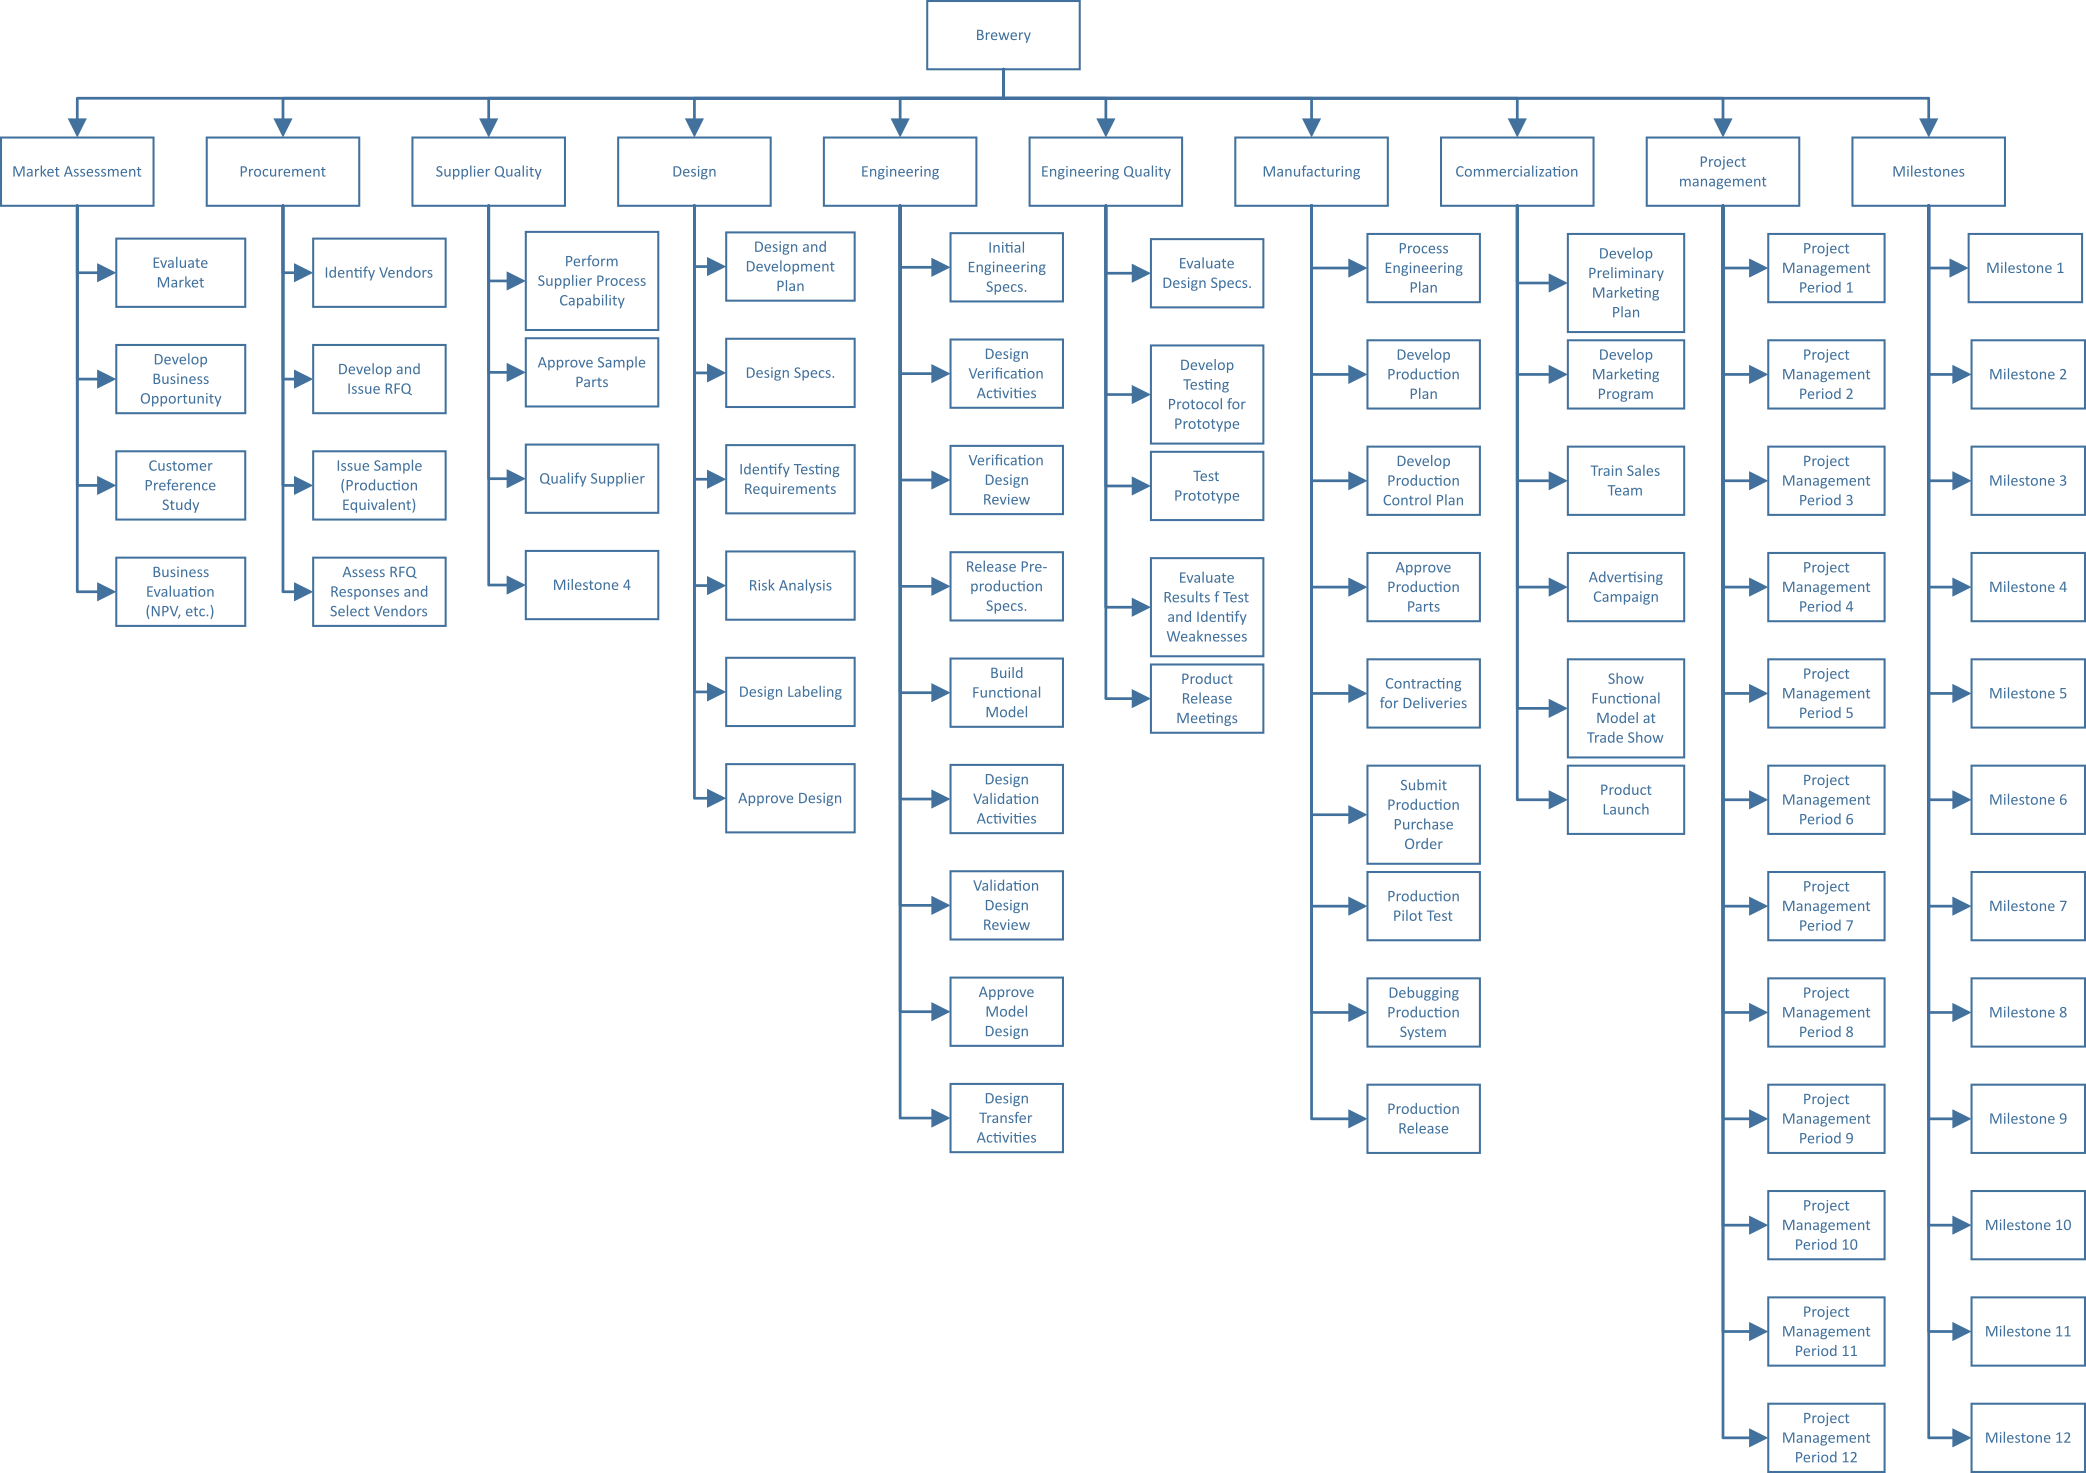
\includegraphics[scale=0.75]{WBS.png}
%\includesvg[scale=0.65,angle=90,origin=c]{WBS}
\caption{Work Breakdown Structure}
\label{fig:wbs}
\end{figure}

\end{landscape}

% geometry end
\restoregeometry

\subsection{Work Responsibilities of disciplinary}

\textbf{Sarel Swart – Process Engineer}\\
\noindent
It will be the work of the process engineer to develop the process that needs to be followed from start to finish of the beer brewery production. This engineer will identify the different ingredients that will have to be added and processes during the development of this product. The engineer will identify the different stages of the process such as malting, mashing and fermentation process.\\

\noindent
\textbf{Biancé Huysamen – Civil Engineer}\\
\noindent
The engineer will have the responsibility of designing the factory/ building of the brewery. A finished building will be renovated and adapted to fit the purpose of a brewery. It is also necessary to use natural lighting and environmentally friendly materials for the building in the most cost efficient way. Civil engineers are also skilled in communicating with different parties. Huysamen also exhibits good financial qualities and will therefore be responsible for the setting up the budget.\\

\noindent
\textbf{Daniel Robinson \& Eduard van der Merwe – Electrical Engineers}\\
\noindent
The brewery will be controlled by electronic systems that have to be developed and programmed. It will be the responsibility of the engineer to update this and ensure the working of the different machinery of the processes and assist will all the programming of the project. Electrical engineers also are focused on detail and therefore Robinson will act as the Quality engineer whilst van der Merwe will assist with the risk analysis.\\

\noindent
\textbf{Carmen Steyn – Industrial Engineer}\\
\noindent
The engineer will ensure that the whole project will run smoothly and will have a broad overview of the project. Industrial engineers are skilled in optimizing systems. The engineer will help with the efficiency of the production process. It’s important that a logical process is developed and designed. The engineer will also oversee the administrative and financial aspects of the project, since industrial engineers are exposed to the business aspects. Steyn will therefore also focus on Marketing and Commercialization.\\

\noindent
\textbf{Peter Toulouras – Mechanical Engineer}\\
\noindent
Toulouras will be responsible for the designing of the different machinery, pumps and tanks that will be used in the brewery process. Toulouras also exhibits great leadership, communication and delegation skills and therefore will fulfill the position of Project leader. It is the responsibility of the project leader to ensure that deadlines are met, that the clients are happy and that the project stays within budget and timeline. Therefore Toulouse will assist with running the entire project.


\subsection{Technical Requirements}
\subsubsection{Summary of product}

There are four types of beer that need to be manufactured namely: Weiss, Ale and two different flavoured lagers. All the beers utilize the same brewing system with slight alterations needed to create each unique beer. These alterations include different fermenting processes and different grains used. There needs to be four brewing systems working simultaneously in order to produce a sufficient amount of all beers. 

\subsubsection{Product Requirements}

\begin{itemize}
\item There should be 4 varieties of beer
\item Each beer will be sold in 500ml glasses
\item The temperature of the beer should always be carefully monitored from the brewing process until the product is sold to the customer 
\item Control systems should be put in place in order to monitor and control each stage of the brewing process 
\item The quality of the final product needs to be of a high standard in order to compete in the respective market 
\item The  final product should be marked at a reasonable price in order to appeal to a wider target market (students)
\item The process compromises of 12 stages that need to be carefully executed in order to produce the best possible product 
\end{itemize}
\subsubsection{Project Requirements}

\begin{itemize}
\item Project commences $15^{th}$ February 2017 and terminates $31^{st}$ January 2018.
\item All the suppliers of the company should be identified and have their capabilities assessed 
\item The final product must be designed completely. The components should include specifications, risk analysis, design analysis, production process and possible testing requirements.
\item A full quality assessment must be done throughout all stages of production of the final product
\end{itemize}

\subsection{Project Limitations}

Limitations are either external or internal constraints placed on the project. In this project the limitations will be:
\begin{itemize}
\item	Cost – the project must be completed within the budget of \$380 000.
\item	Time – the project must be completed within the given time frame.
\item	Availability of required equipment and ingredients for the brewing process.
\item	Workforce/employees that will not work as efficiently as they possibly can.
\item	Unavailability of resources due to unforeseen circumstances.
\item	Construction limitations due to equipment being produced offsite – Difficulties in its transportation.
\item	Waiting Period to ensure a valid liquor licence from the National Liquor Authority which is a regulatory body within the Department of Trade and Industry (DTI) responsible for administering The National Liquor Act
\item	Workforce rights – influence on production and employment costs
\item	Environmental responsibility - The entire project must have a minimal effect on the environment.
\item	Specific standards and regulations – The overall project must adhere to all relevant standards and regulations to ensure legal rights.
\item	Size of the building itself – Since it is a small local brewing company, the company only caters for a limited number of people. This means that there are limited staff members.
\item	Can only have a limited number of vats that fit inside the building. This means that only a limited amount of beer will be processed at a time, which leads to not being able to supply large quantities of beer at a time.
\item	Beer brewing takes time – One cannot produce beverages out of a vat too early.
\item	Construction/building takes time – one needs enough capital for delays.
\item	Marketing – Needs to be well marketed to ensure that the company makes a profit.
\item	Health and safety regulations – Needs a fire exit and all the necessary precautions to ensure the safety of everyone in and around the building.
\item	Limited parking space – Needs enough parking for at least 30\% of the customers at all times.
\item	Enough restrooms will be needed – Takes up space but it is crucial – could lead to unhappy staff that has to clean up after messy students.
\item	Competition – The price and the taste of the beer have to be on par or better than its rival companies.
\end{itemize}
%
%
\subsection{Project Exclusions}
These are often referred to as the project boundaries. Exclusions are components of the system in which the project is completed that will not be addressed by the project. These will include\\
\begin{itemize}
\item	Maintenance, upgrading and operation of the brewing process.
\item	The availability of supporting infrastructure at the construction site (water pipes, power lines, access roads etc.)
\item	The project does not invest in broadening the variety of beers made.
\item	Municipal approval and authorization on project operations.
\item	Damage or theft of customer’s belongings – Everything is at their own risk.
\end{itemize}

%\subsection{Limits and Exclusions}
%\subsubsection{Limits}
%\subsubsection{Exclusions}

\subsection{Review and Approval} 

When developing a product or service for a client it is very important to keep client satisfaction in mind. If the client is not happy then there the feasibility of the project in general is compromised. If the project is not feasible there is market for the product or service because the customers will not buy it. This is why it is very important to do a feasibility study early on in the process. The feasibility study must ensure that the customer will be willing to spend money on this product or service. To determine if the product will be feasible the customer must evaluate the following; cost, the benefits of the project, the likelihood that the project will succeed and the reputation of the contractor that is used for the project.\\

\noindent
To be able to do a feasibility study all of the phases in the process need to be documented. These documents need to contain diagrams and schematic representations of the entire process and all the steps and resources that were used. By documenting everything it is easier for the customer to review all of the decisions made. It can also make it easier to see why these decisions were made. By making it easier for the customer to review the projects progress the contractor can be ensured of customer satisfaction. Customer approval procedure must be done regularly throughout the process, this ensures that if there are any errors early on in the process, they can be evaluated and alternative solutions can be made. By doing this regularly the contractor can ensure that the client stays satisfied throughout the process. If these errors are picked up early it can save the contractor a lot of money later in the process.

\newpage
\section{Project Baseline Plan}
\subsection{Baseline Commentary}

A baseline following almost 40\% quicker estimates compared to the original simulation estimates, seems to correlate well with the simulated runs. However, some slack is required for a successful project. At least two weeks are given as leeway. Although the project is run tightly, it is justified due to the competitive nature of the project.\\

\noindent
See Appendix \ref{appendix:baseline} for the project baseline.

\section{Project Budget}

The estimated budget and estimated hours provided by Sim4project was used as a guideline of what should be spent during each period to ensure that the project would stay within the budget of \$380 000.\\

\noindent
To calculate the budget the effectiveness of the resources were brought into consideration. An assumption was made that all resources will work at an 80\% effectiveness rate. The estimated hours of each task as well as the safety margin of 80\% effectiveness was used to determine the hours worked for each task using the formula provided.


\begin{center}
$ Actual\ time\ worked\ (hours)\ =\ \frac{Estimated\ time\ (hours)}{\% effectiveness} $
\end{center}

\noindent
The budget forecast is provided in Appendix \ref{appendix:budget}.

\subsection{Direct Resource Costs}

Table \ref{tab:resourcecosts} provides the estimated cost of the different resources that will be hired. More than one engineer will be hired since the engineer will be working as a Project Manager for the period.

\begin{table}[H]
\centering
\caption{Resource costs per hour}
\label{tab:resourcecosts}
\begin{tabular}{ll}
\textbf{Resources}          & \textbf{Rate} \\\hline
Engineer 1                  & \$58.00       \\
Engineer 2                  & \$42.00       \\
Junior Marketing Specialist & \$57.00       \\
Junior Product designer     & \$47.00       \\
Marketing Manager           & \$95.00       \\
Operation Specialist        & \$53.00       \\
Quality Engineer            & \$71.00       \\
Senior product designer     & \$84.00       \\
Engineer 3                  & \$55.00      
\end{tabular}
\end{table}

\subsection{Training and Events prospective costs}

There was decided that during the first period the engineer will be sent for training on project Management. This is to ensure that the engineer will be more effective as a project Manager. There was also decided to hire resources that are cheaper but have less skills and send them for training to improve their skills and effectiveness.\\

\noindent
Managerial actions will also be rewarded to resources to improve their work ethic and effictiveness.\\

\noindent
Table \ref{tab:actions} provides information regarding the different training and managerial actions that will take place during the provided timeline.

% Please add the following required packages to your document preamble:
% \usepackage[table,xcdraw]{xcolor}
% If you use beamer only pass "xcolor=table" option, i.e. \documentclass[xcolor=table]{beamer}
\begin{table}[]
\centering
\caption{Training and Managerial Actions costs}
\label{tab:actions}
\begin{tabular}{llllll}
\textbf{Period} & \textbf{Action}              & \textbf{Amount of People} & \textbf{Cost} & \textbf{Total Cost}                 &  \\
1               & Project Management           & 1                         & \$1,000.00    & \$1,000.00                          &  \\
                & Project Evaluation           & 1                         & \$1,000.00    & \$1,000.00                          &  \\
3               & Interpersonal training       & 2                         & \$600.00      & \$1,200.00                          &  \\
5               & company sponsored event      & 3                         & \$100.00      & \$300.00                            &  \\
6               & Pizza Party                  & 6                         & \$10.00       & \$60.00                             &  \\
                & Process Engineering          & 1                         & \$600.00      & \$600.00                            &  \\
8               & Management Recognition event & 4                         & \$50.00       & \$200.00                            &  \\
9               & Pizza Party                  & 6                         & \$10.00       & \$60.00                             &  \\
                & Negotiation techniques       & 2                         & \$600.00      & \$1,200.00                          &  \\
10              & Principles of Quality        & 1                         & \$600.00      & \$600.00                            &  \\
                & Pizza Party                  & 8                         & \$10.00       & \$80.00                             &  \\
11              & Milestone celebration        & 4                         & \$1,000.00    & \$4,000.00                          &  \\
                &                              &                           &               & \cellcolor[HTML]{FFFE65}\$10,300.00 & 
\end{tabular}
\end{table}

\subsection{Total Costs}

The total cost estimate of each period is listed in the table below. %(figure) \ref{fig:totalcosts}.

\begin{figure}[H]
\centering
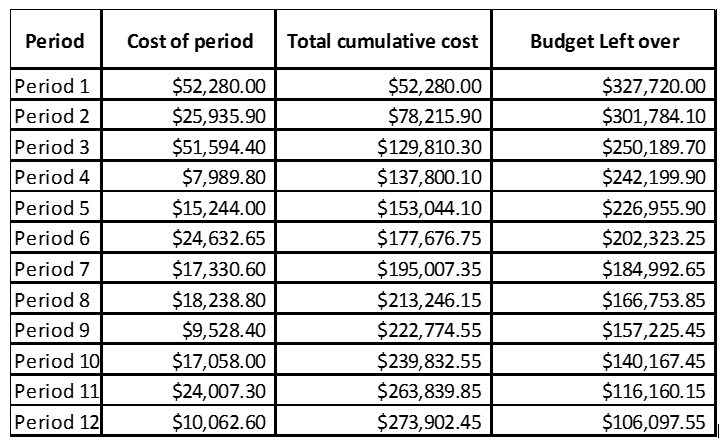
\includegraphics[scale=0.6]{images/totalcost.png}
\label{fig:totalcosts}
\caption{Total costs for periods}
\end{figure}

%% Please add the following required packages to your document preamble:
%% \usepackage[table,xcdraw]{xcolor}
%% If you use beamer only pass "xcolor=table" option, i.e. \documentclass[xcolor=table]{beamer}
%\begin{table}[]
%\centering
%\caption{Total estimated costs}
%\label{tab:totalcosts}
%\begin{tabular}{llllll}
%\textbf{Period} & \textbf{Cost of period} & \textbf{Total cumulative cost} & \textbf{Budget Left over}           &  &  \\
%Period 1        & \$57,920.00             & \$57,920.00                    & \$322,080.00                        &  &  \\
%Period 2        & \$43,560.00             & \$101,480.00                   & \$278,520.00                        &  &  \\
%Period 3        & \$60,420.00             & \$161,900.00                   & \$218,100.00                        &  &  \\
%Period 4        & \$15,535.00             & \$177,435.00                   & \$202,565.00                        &  &  \\
%Period 5        & \$19,185.00             & \$196,620.00                   & \$183,380.00                        &  &  \\
%Period 6        & \$30,561.25             & \$227,181.25                   & \$152,818.75                        &  &  \\
%Period 7        & \$18,865.00             & \$246,046.25                   & \$133,953.75                        &  &  \\
%Period 8        & \$17,420.00             & \$263,466.25                   & \$116,533.75                        &  &  \\
%Period 9        & \$10,850.00             & \$274,316.25                   & \$105,683.75                        &  &  \\
%Period 10       & \$16,990.00             & \$291,306.25                   & \$88,693.75                         &  &  \\
%Period 11       & \$27,452.50             & \$318,758.75                   & \$61,241.25                         &  &  \\
%Period 12       & \$14,660.00             & \$333,418.75                   & \cellcolor[HTML]{9AFF99}\$46,581.25 &  &  \\
%                &                         &                                &                                     &  & 
%\end{tabular}
%\end{table}

\noindent
The budget estimates that a surplus of \$106 097.55 will be left over. 

\newpage
\section{Risk Analysis}

All risks pertaining to the simulator and product were identified and evaluated from project analogy. These risks were classified as internal or external based on the risk source, with 25 risk identified for each category. These risks were compiled and analysed in a special risk management meeting wherein the risks were identified and allocated to two group members to analyse in further detail. The minutes of the meeting may be found in Appendix \ref{appendix:minutes}.\\

\noindent
A comprehensive summary of the project risk may be found in Appendix \ref{appendix:projectrisks}. The risk rank, management strategy, and frequency are shown for each risk identified. The risk management strategy are classified as risk acceptance, risk control, risk avoidance, and contingency plan. This includes a more detailed summary of the risk response for each risk.\\

\noindent
The risks were identified through project analogy wherein the risks were classified according risk source. Risk assessment was carried out using a double variable five point scale method. The two factors considered were the probability of the risk occurring, and the impact of the realisation of the risk on the project. The evaluation scale ranged from very high (5) to very low(1). These factors are combined by multiplication to yield an overall rank for each risk. Table \ref{appendix:riskmatrix} shows the risk evaluation matrix used with colour codes used to indicate the severity of the risk. 


\newpage
%\section*{Appendices}
\begin{appendices}
%\subsection*{Appendix A: Budget Documentation and Analysis}
\section{Budget Documentation and Analysis}
\label{appendix:budget}

\subsection{Simulated Task Estimations}

\begin{figure}[H]
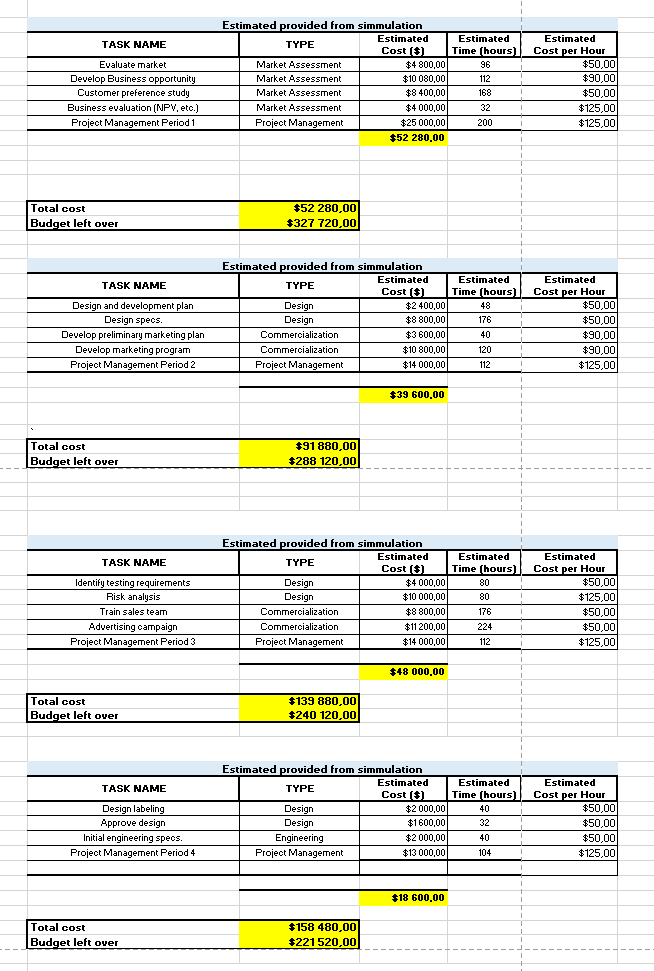
\includegraphics[scale=0.75]{forecast/budget_forecast_sim_1234.PNG}
\caption{Budget Forecast from simulation (periods 1 - 4)}
\end{figure}
\begin{figure}[H]
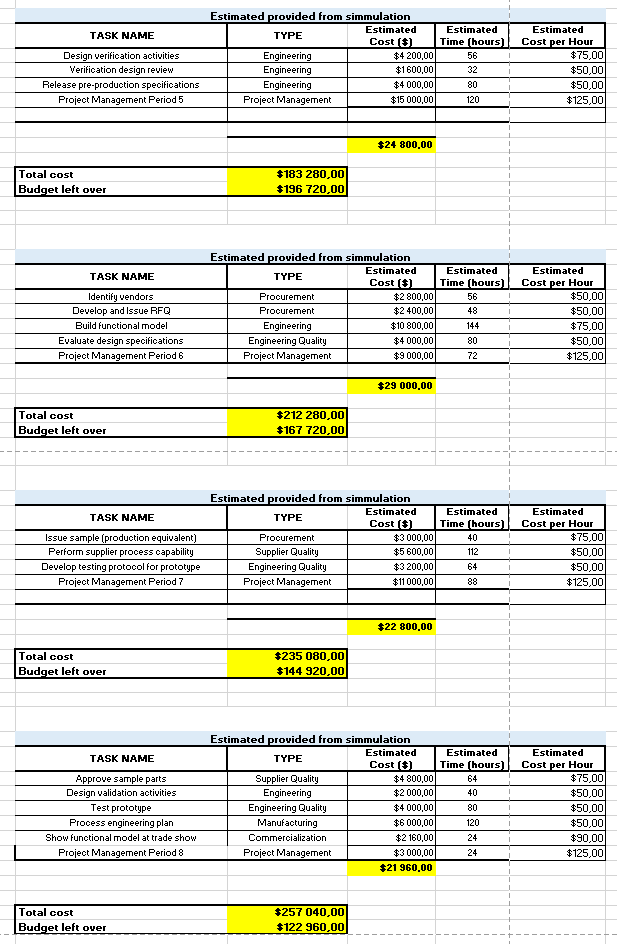
\includegraphics[scale=0.8]{forecast/budget_forecast_sim_5678.PNG}
\caption{Budget Forecast from simulation (periods 5 - 8)}
\end{figure}
\begin{figure}[H]
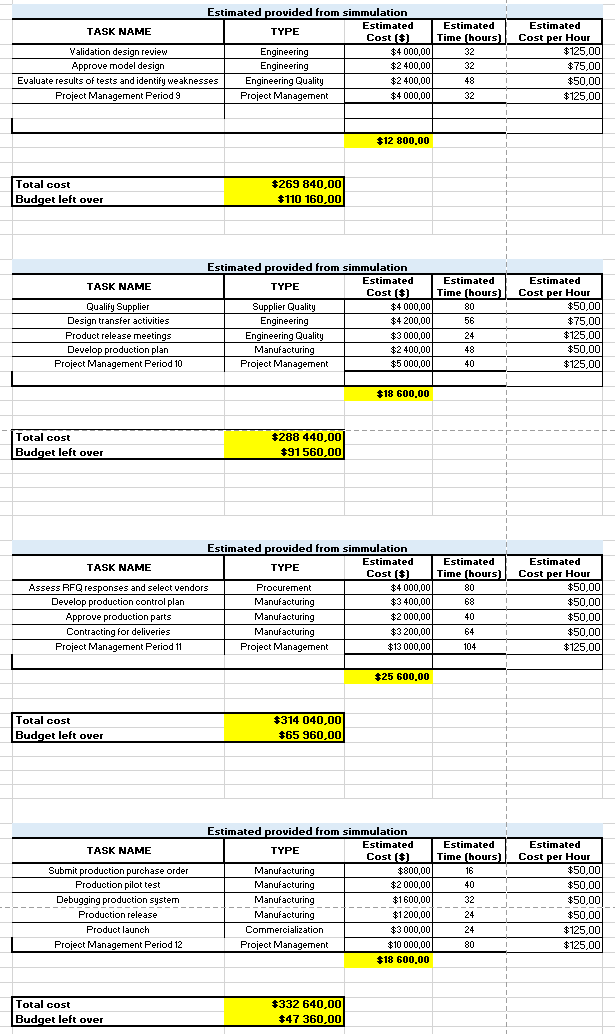
\includegraphics[scale=0.8]{forecast/budget_forecast_sim_9101112.PNG}
\caption{Budget Forecast from simulation (period 9 - 12)}
\end{figure}
%\begin{figure}[H]
%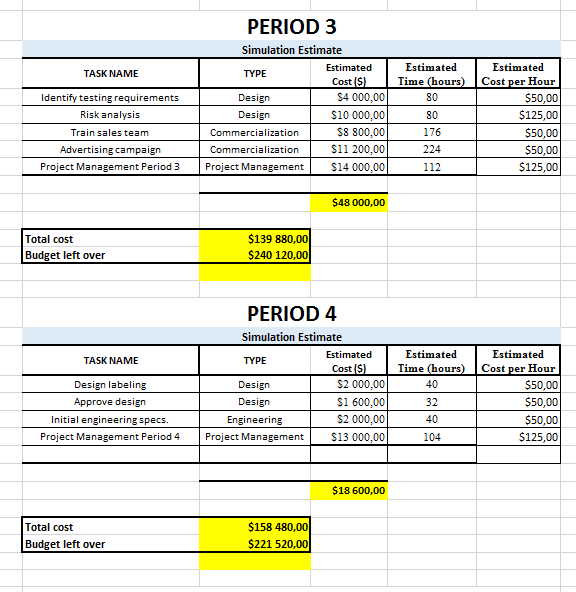
\includegraphics[scale=1]{forecast/budget_forecast_sim_34.PNG}
%\caption{Budget Forecast from simulation (period 3 and 4)}
%\end{figure}
%\begin{figure}[H]
%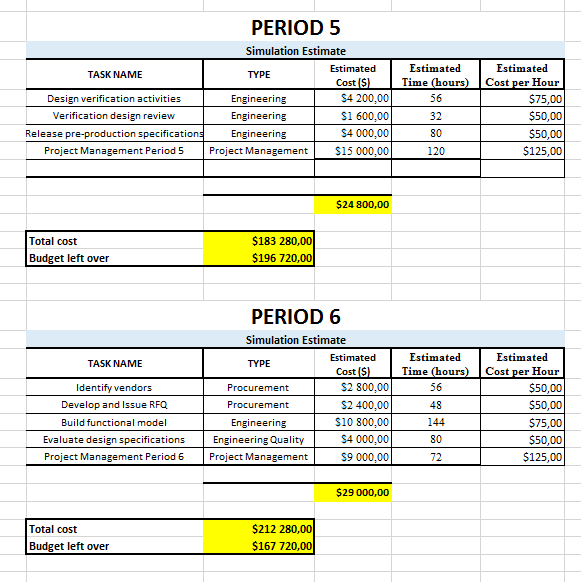
\includegraphics[scale=1]{forecast/budget_forecast_sim_56.PNG}
%\caption{Budget Forecast from simulation (period 5 and 6)}
%\end{figure}
%\begin{figure}[H]
%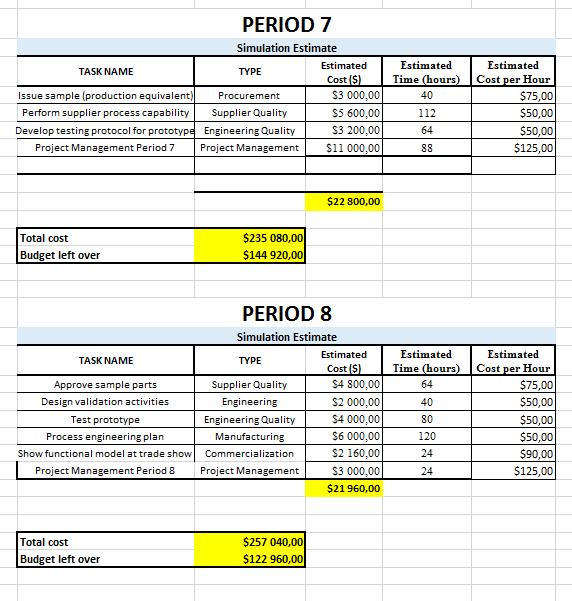
\includegraphics[scale=1]{forecast/budget_forecast_sim_78.PNG}
%\caption{Budget Forecast from simulation (period 7 and 8)}
%\end{figure}
%\begin{figure}[H]
%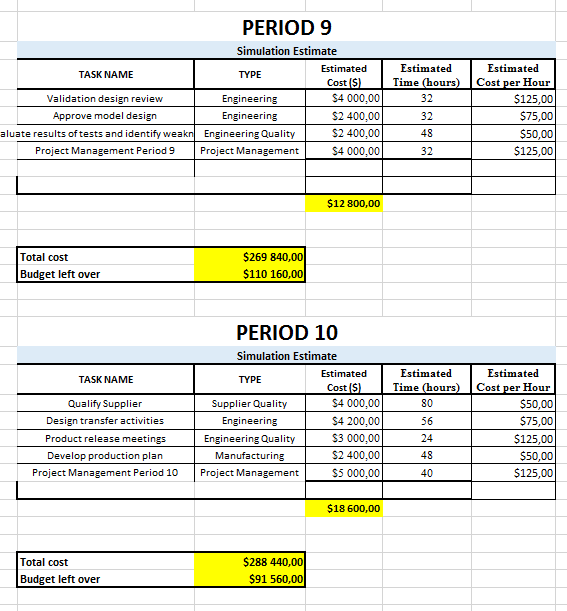
\includegraphics[scale=1]{forecast/budget_forecast_sim_910.PNG}
%\caption{Budget Forecast from simulation (period 9 and 10)}
%\end{figure}
%\begin{figure}[H]
%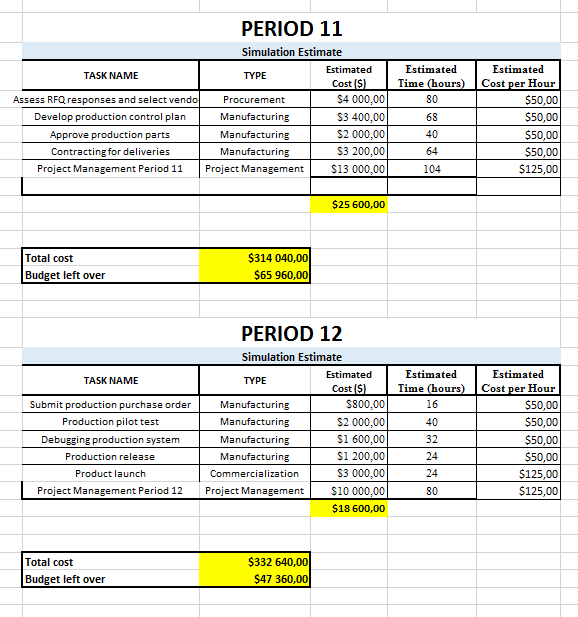
\includegraphics[scale=1]{forecast/budget_forecast_sim_1112.PNG}
%\caption{Budget Forecast from simulation (period 11 and 12)}
%\end{figure}

\begin{landscape}

\subsection{Direct Resource, Managerial and Training Costs}

\begin{figure}[H]
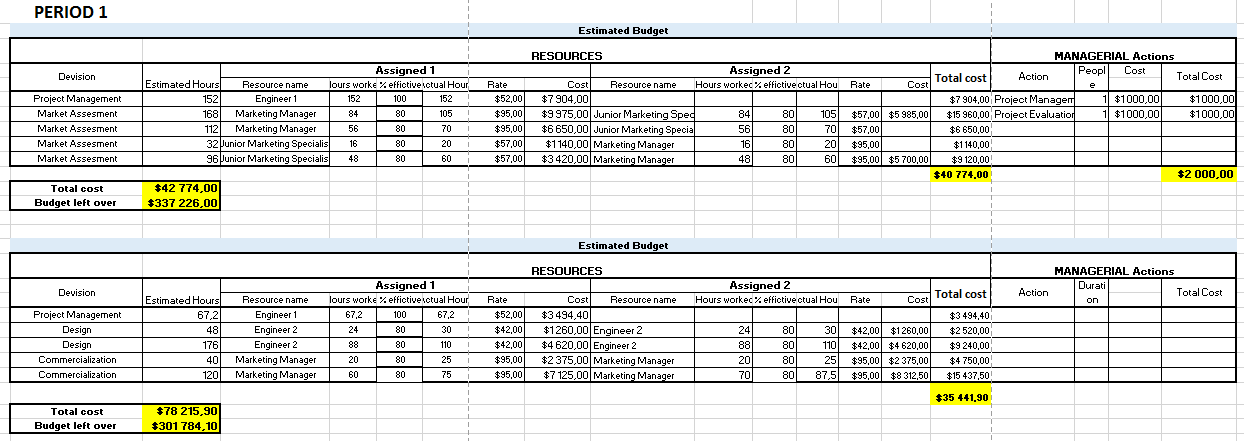
\includegraphics[scale=0.75]{forecast/budget_forecast_est_12.PNG}
\caption{Budget Forecast from estimation (period 1 and 2)}
\end{figure}
\begin{figure}[H]
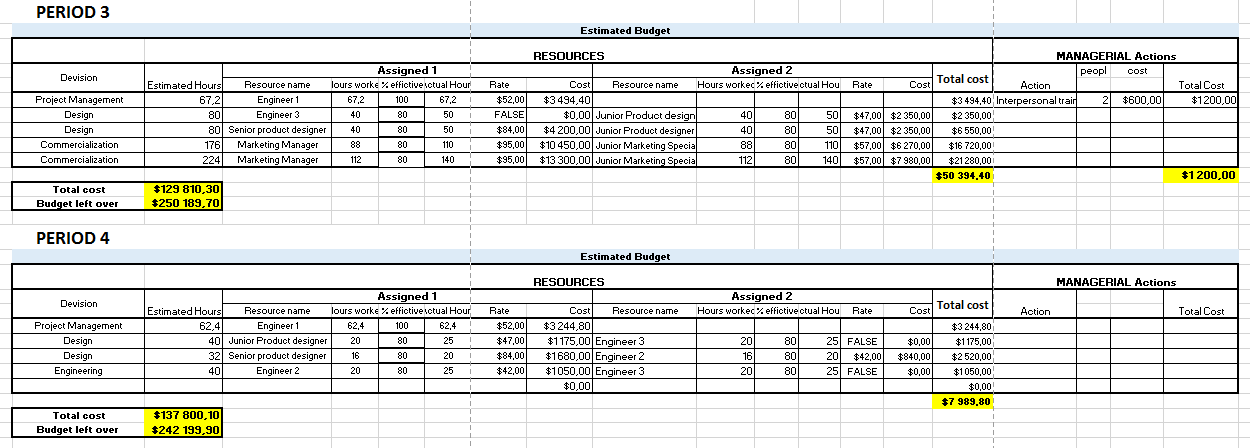
\includegraphics[scale=0.8]{forecast/budget_forecast_est_34.PNG}
\caption{Budget Forecast from estimation (period 3 and 4)}
\end{figure}
\begin{figure}[H]
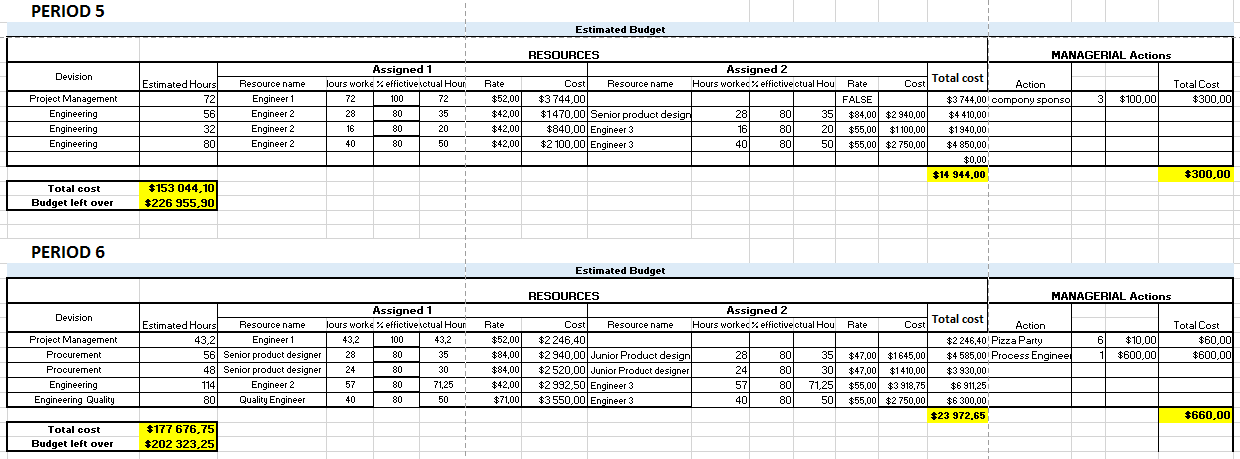
\includegraphics[scale=0.8]{forecast/budget_forecast_est_56.PNG}
\caption{Budget Forecast from estimation (period 5 and 6)}
\end{figure}
\begin{figure}[H]
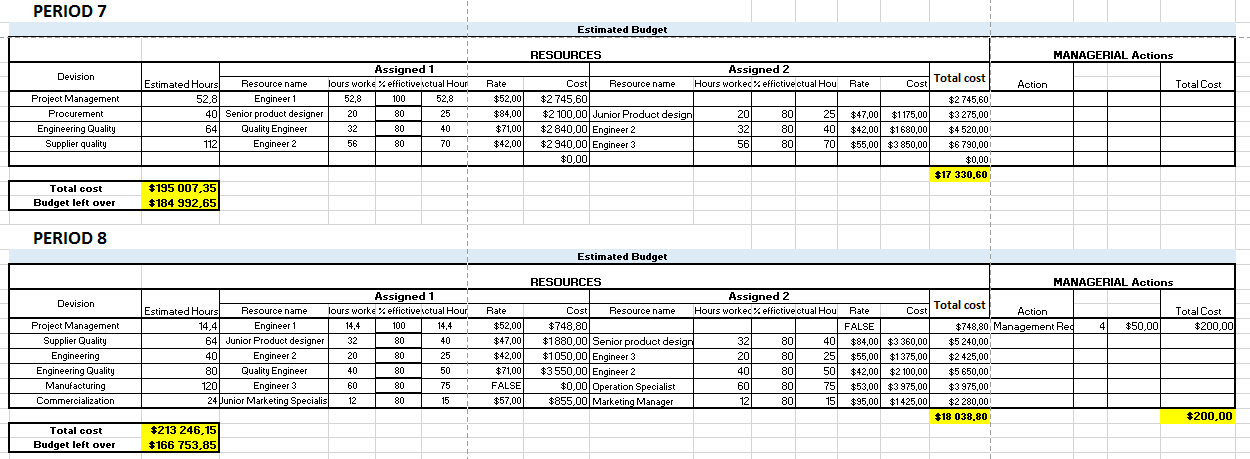
\includegraphics[scale=0.8]{forecast/budget_forecast_est_78.PNG}
\caption{Budget Forecast from estimation (period 7 and 8)}
\end{figure}
\begin{figure}[H]
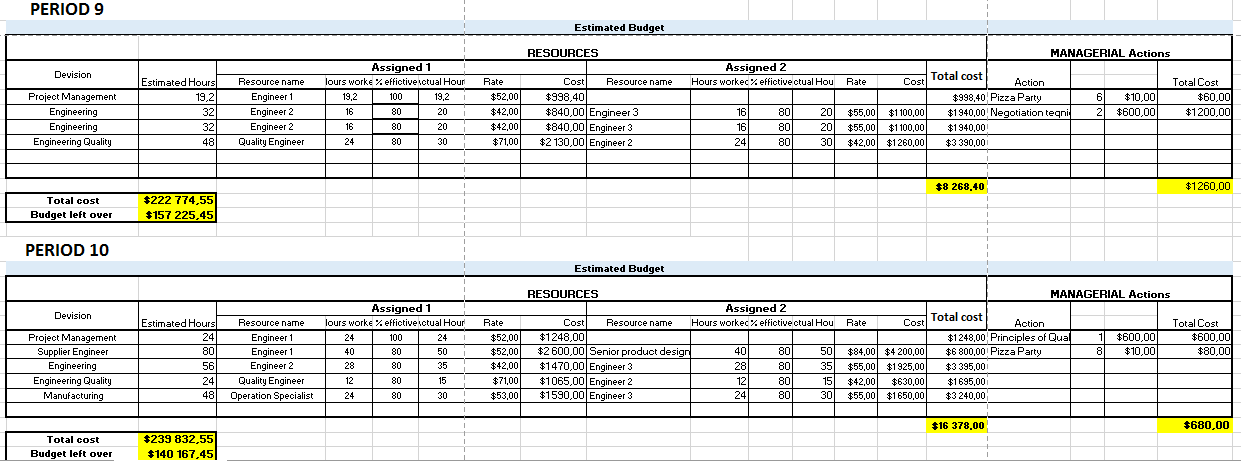
\includegraphics[scale=0.8]{forecast/budget_forecast_est_910.PNG}
\caption{Budget Forecast from estimation (period 9 and 10)}
\end{figure}
\begin{figure}[H]
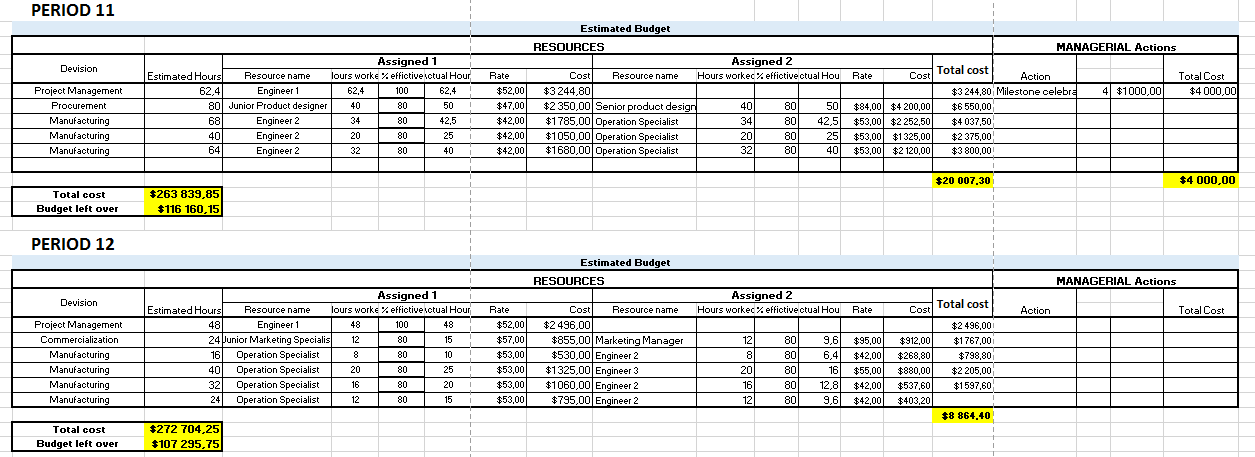
\includegraphics[scale=0.8]{forecast/budget_forecast_est_1112.PNG}
\caption{Budget Forecast from estimation (period 11 and 12)}
\end{figure}

\end{landscape}

\begin{landscape}

\section{Risk Register}
\subsection{Risk Assessment Plan}
\label{appendix:projectrisks}

% Please add the following required packages to your document preamble:
% \usepackage{graphicx}
% \usepackage[table,xcdraw]{xcolor}
% If you use beamer only pass "xcolor=table" option, i.e. \documentclass[xcolor=table]{beamer}
\begin{table}[H]
\centering
\caption{Internal Project Risks}
\label{tab:internal}
\resizebox{1.79\textwidth}{!}{%
\begin{tabular}{lllllll}
Risks & Probability & Impact & Risk Rank & Risk Response Strategy & Risk Management & Expected Frequency \\
Overestimation of resource effectiveness leading to delays & 4 & 4 & \cellcolor[HTML]{F56B00}16 & Contingency Plan & Reassess resource capability and change taks allocation strategy. & Every Period \\
Budget Cuts & 4 & 4 & \cellcolor[HTML]{F56B00}16 & Contingency Plan & Revise budget, and redirect costs where necessary. Allocate funds for unexpected costs in budget. & Once-off \\
Mismanagement causing demotivation and inefficiency & 4 & 3 & \cellcolor[HTML]{F8FF00}12 & Contingency Plan & Take managerial action. Consider reallocating or terminating resource employment. & Quarterly \\
Idle/Un-allocated resources & 3 & 4 & \cellcolor[HTML]{F8FF00}12 & Contingency Plan & Consider firing idle resources. & Monthly \\
Product causes legal liability & 2 & 5 & \cellcolor[HTML]{F8FF00}10 & Risk Avoidance & Maintain strict product quality procedures and tests & Once-off \\
Bad working relationships between resources. & 3 & 3 & \cellcolor[HTML]{F8FF00}9 & Contingency Plan & Take managerial action. Consider reallocating or terminating resource employment. & Monthly \\
Low paid workers causing low effectiveness & 3 & 3 & \cellcolor[HTML]{F8FF00}9 & Contingency Plan & Allocate funds for pay raises if necessary. & Yearly \\
Inaccurate cost estimate & 3 & 3 & \cellcolor[HTML]{F8FF00}9 & Risk Avoidance & Add contingency to budget. Use locally available equipment instead of importing. & Once-off \\
Resources inexperienced & 3 & 3 & \cellcolor[HTML]{F8FF00}9 & Contingency Plan & Pair inexperienced resources up to allow for lower efficiency & Quaterly \\
Unflexible design & 3 & 3 & \cellcolor[HTML]{F8FF00}9 & Contingency Plan & Identify problematic process areas, and consult specialist for possible solutions. & Once-off \\
Recruiting process incurrs delays & 3 & 3 & \cellcolor[HTML]{F8FF00}9 & Risk Avoidance & Ensure critical task resources are hired early to account for a possible delay. & Yearly \\
Extended deadline & 2 & 4 & \cellcolor[HTML]{F8FF00}8 & Risk Acceptance & Evaluate influence on costs and take appropriate action. & Once-off \\
Low communications within project team & 2 & 4 & \cellcolor[HTML]{F8FF00}8 & Risk Avoidance & Set up standard communication platforms. & Once-off \\
Design fails technical review & 2 & 4 & \cellcolor[HTML]{F8FF00}8 & Contingency Plan & Allocate funds to accomodate for project delays & Once-off \\
Monitoring and control components lack stability & 2 & 4 & \cellcolor[HTML]{F8FF00}8 & Contingency Plan & Include testing procedure to identify and assess control system performance. Allocate funding for project delays. & Once-off \\
Unreliable control system & 2 & 4 & \cellcolor[HTML]{F8FF00}8 & Contingency Plan & Include testing procedure to identify and assess control system performance. Allocate funding for project delays. & Once-off \\
Resource training inadequate & 2 & 3 & \cellcolor[HTML]{F8FF00}6 & Risk Avoidance & Send multiple resources for the same training. & Monthly \\
Stake holders become disengaged & 2 & 3 & \cellcolor[HTML]{F8FF00}6 & Risk Control & Meet up with stakeholders and give progress of product development. & Yearly \\
Monitoring and control components are overengineered & 2 & 3 & \cellcolor[HTML]{F8FF00}6 & Risk Avoidance & Maintain conformity to international standards. & Once-off \\
Low moral among resources & 1 & 4 & \cellcolor[HTML]{34FF34}4 & Contingency Plan & Tank managerial action (pizza party) & Monthly \\
Infeasible design & 1 & 4 & \cellcolor[HTML]{34FF34}4 & Risk Control & Extend design period. Allocate more resources. & Once-off \\
Design not fit for purpose & 1 & 4 & \cellcolor[HTML]{34FF34}4 & Riks Avoidance & Set up a testing procedure to identify problematic areas. & Once-off \\
Monitoring and control components not fit for purpose & 1 & 4 & \cellcolor[HTML]{34FF34}4 & Risk Avoidance & Set up a testing procedure to identify problematic areas. & Once-off \\
Loss of intellectual property & 1 & 3 & \cellcolor[HTML]{34FF34}3 & Risk Avoidance & Inform resources on a need-to-know basis regarding processing specifics. & Once-off
\end{tabular}%
}
\end{table}

% Please add the following required packages to your document preamble:
% \usepackage{graphicx}
% \usepackage[table,xcdraw]{xcolor}
% If you use beamer only pass "xcolor=table" option, i.e. \documentclass[xcolor=table]{beamer}
\begin{table}[H]
\centering
\caption{External Project Risks}
\label{my-label}
\resizebox{1.79\textwidth}{!}{%
\begin{tabular}{lllllll}
Risks & Probability & Impact & Risk Rank & Risk Response Strategy & Risk Management & Expected Frequency \\
Legal \& regulatory changes & 4 & 5 & \cellcolor[HTML]{F56B00}20 & Risk Avoidance & Anticipate legal and regulatory changes, and make provisions based on forecasts. Seek professional legal advice. & Yearly \\
Strike causes delays & 4 & 4 & \cellcolor[HTML]{F56B00}16 & Contingency Plan & Assessing the time lost, if any, and determine strategy to make-up for delay in next period. Allocate funds for unexpected costs in budget. & Once-off \\
Low product demand & 3 & 5 & \cellcolor[HTML]{F56B00}15 & Risk Control & Develop marketing strategy for product promotion & Once-off \\
Low quality infrastructure & 3 & 4 & \cellcolor[HTML]{F8FF00}12 & Risk Control & Work closely with manicipality and surrounding businesses for improvement of relevant infrastructure. & Once-off \\
Market changes & 4 & 3 & \cellcolor[HTML]{F8FF00}12 & Risk Control & Monitor market trends, and keep design flexible for process and supplier changes & Yearly \\
Vendors start late & 3 & 4 & \cellcolor[HTML]{F8FF00}12 & Contingency Plan & Allocate funds to accomodate for project delays & Once-off \\
Required resources not available & 2 & 5 & \cellcolor[HTML]{F8FF00}10 & Contingency Plan & Hire alternative resources, and send for appropriate training. & Once-off \\
Response to RFP of low quality & 3 & 3 & \cellcolor[HTML]{F8FF00}9 & Risk Control & Send RFP to international companies to assess alternatives proposals. & Once-off \\
Low service quality & 3 & 3 & \cellcolor[HTML]{F8FF00}9 & Contingency Plan & Allocate reserve funds for delay. Consider changing service provider. & Once-off \\
Training delay & 3 & 3 & \cellcolor[HTML]{F8FF00}9 & Risk Acceptance & Allow extra time for training. & Once-off \\
Sudden property price increase & 3 & 3 & \cellcolor[HTML]{F8FF00}9 & Contingency Plan & Consider hiring options for brewery site. & Yearly \\
Power Failures & 2 & 4 & \cellcolor[HTML]{F8FF00}8 & Contingency Plan & Check load shedding notifications. Hire generators when neccessary. & Monthly \\
Vendor components fail to meet requirements & 2 & 4 & \cellcolor[HTML]{F8FF00}8 & Contingency Plan & Make contact with another vendor as soon as possible. Allocate funds for unwanted costs. Seek legal advice. & Once-off \\
Low quality vendor components & 2 & 4 & \cellcolor[HTML]{F8FF00}8 & Contingency Plan & Send items back to vendor if they do not adhere to requiments in contract. Allocate funds for project delays. & Once-off \\
Unplanned leave for resources & 2 & 4 & \cellcolor[HTML]{F8FF00}8 & Contingency Plan & Consider re-allocation of available resources or hiring tempory resources. & Once-off \\
Demage to facilities due to fire & 2 & 4 & \cellcolor[HTML]{F8FF00}8 & Risk Avoidance & Install fire exstinghuisers throughout facililties & Once-off \\
Petrol Price Increases & 4 & 2 & \cellcolor[HTML]{F8FF00}8 & Contingency Plan & Consider searching for closer main suppliers. & Yearly \\
Contract terms and price unreasonable & 2 & 3 & \cellcolor[HTML]{F8FF00}6 & Risk Control & Make contact with other local or international suppliers. &  \\
Unexpected legal action against company causing delays and cost increases. & 2 & 3 & \cellcolor[HTML]{F8FF00}6 & Risk Acceptance & Allocate funds for unforeseen cost increaases. & Once-off \\
Unexpected brewery site change. & 2 & 3 & \cellcolor[HTML]{F8FF00}6 & Contingency Plan & Keep list of possible alternative sites for brewery. & Yearly \\
Exchange rate & 4 & 1 & \cellcolor[HTML]{34FF34}4 & Risk Avoidance & Provide reserve fund for cost increases associated with exchange rate instability. Use local vendors. & Once-off \\
No response to RFP & 1 & 3 & \cellcolor[HTML]{34FF34}3 & Contingency Plan & Extend RFP internationally to possibly import. & Once-off \\
Conflict between vendors & 1 & 3 & \cellcolor[HTML]{34FF34}3 & Risk Avoidance & Review contracts and schedules to avoid clashes between vendors caused by misanderstandings. & Once-off \\
Material Cost Increases for Prototype & 3 & 1 & \cellcolor[HTML]{34FF34}3 & Risk Control & Explore other material suppliers. & Once-off
\end{tabular}%
}
\end{table}

% Please add the following required packages to your document preamble:
% \usepackage{graphicx}
% \usepackage[table,xcdraw]{xcolor}
% If you use beamer only pass "xcolor=table" option, i.e. \documentclass[xcolor=table]{beamer}
%\begin{table}[H]
%\centering
%\caption{Project Risks}
%\label{tab:projectrisks}
%\resizebox{1.79\textwidth}{!}{%
%\begin{tabular}{lllllll}
%\hline
%Risks & Probability & Impact & Risk Rank & Risk Response Strategy & Risk Management & Expected Frequency \\ \hline
%Overestimation of resource effectiveness leading to delays & 4 & 4 & 16 & \cellcolor[HTML]{F56B00}Contingency Plan & Reassess resource capability and change taks allocation strategy. & Every Period \\
%Budget Cuts & 4 & 4 & 16 & \cellcolor[HTML]{F56B00}Contingency Plan & Revise budget, and redirect costs where necessary. Allocate funds for unexpected costs in budget. & Once-off \\
%Mismanagement causing demotivation and inefficiency & 4 & 3 & 12 & \cellcolor[HTML]{F8FF00}Contingency Plan & Take managerial action. Consider reallocating or terminating resource employment. & Quarterly \\
%Required resources not available & 2 & 5 & 10 & \cellcolor[HTML]{F8FF00}Contingency Plan & Hire alternative resources, and send for appropriate training. & Once-off \\
%Low effectiveness & 2 & 5 & 10 & \cellcolor[HTML]{F8FF00}Risk Control & Make sure critical path stays protected. & Once-off \\
%Training delay & 3 & 3 & 9 & \cellcolor[HTML]{F8FF00}Risk Acceptance & Allow extra time for training. & Once-off \\
%Unplanned leave for resources & 2 & 4 & 8 & \cellcolor[HTML]{F8FF00}Contingency Plan & Consider re-allocation of available resources or hiring tempory resources. &  \\
%Extended deadline & 2 & 4 & 8 & \cellcolor[HTML]{F8FF00}Risk Acceptance & Evaluate influence on costs and take appropriate action. & Once-off \\
%Resource training inadequate & 2 & 3 & 6 & \cellcolor[HTML]{F8FF00}Risk Avoidance & Send multiple resources for the same training. & Monthly \\
%Low moral mong resources & 1 & 4 & 4 & \cellcolor[HTML]{34FF34}Contingency Plan & Tank managerial action (pizza party) & Monthly \\
% &  &  &  &  &  &  \\
% &  &  &  &  &  &  \\
% &  &  &  &  &  &  \\
% &  &  &  &  &  &  \\
% &  &  &  &  &  &  \\
% &  &  &  &  &  &  \\
% &  &  &  &  &  &  \\
% &  &  &  &  &  &  \\
% &  &  &  &  &  &  \\
% &  &  &  &  &  &  \\
% &  &  &  &  &  &  \\
% &  &  &  &  &  &  \\ \hline
%\end{tabular}%
%}
%\end{table}

\end{landscape}


%%%%%%%%%%%%%%%%%%%%%%%%%%%%%%%%%%%%%%%%%%%%%%%%%%%%%%%%%%%%%

%\begin{landscape}
%
%\subsection{Risk identification}
%
%% Please add the following required packages to your document preamble:
%% \usepackage{graphicx}
%% \usepackage[table,xcdraw]{xcolor}
%% If you use beamer only pass "xcolor=table" option, i.e. \documentclass[xcolor=table]{beamer}
%\begin{table}[H]
%\centering
%\caption{Product Risks}
%\label{tab:productrisks}
%\resizebox{1.75\textwidth}{!}{%
%\begin{tabular}{lllllll}
%Risks & Probability & Impact & Risk Rank & Risk Response Strategy & Risk Management & Expected Frequency \\
%Legal \& regulatory changes & 4 & 5 & \cellcolor[HTML]{F56B00}20 & Risk Avoidance & Anticipate legal and regulatory changes, and make provisions based on forecasts. Seek professional legal advice. & Yearly \\
%Low product demand & 3 & 5 & \cellcolor[HTML]{F56B00}15 & Risk Control & Develop marketing strategy for product promotion & Once-off \\
%Low quality infrastructure & 3 & 4 & \cellcolor[HTML]{F8FF00}12 & Risk Control & Work closely with manicipality and surrounding businesses for improvement of relevant infrastructure. & Once-off \\
%Market changes & 4 & 3 & \cellcolor[HTML]{F8FF00}12 & Risk Control & Monitor market trends, and keep design flexible for process and supplier changes & Yearly \\
%Vendors start late & 3 & 4 & \cellcolor[HTML]{F8FF00}12 & Contingency Plan & Allocate funds to accomodate for project delays & Once-off \\
%Product causes legal liability & 2 & 5 & \cellcolor[HTML]{F8FF00}10 & Risk Avoidance & Maintain strict product quality procedures and tests & Once-off \\
%Response to RFP of low quality & 3 & 3 & \cellcolor[HTML]{F8FF00}9 & Risk Control & Send RFP to international companies to assess alternatives proposals. & Once-off \\
%Inaccurate cost estimate & 3 & 3 & \cellcolor[HTML]{F8FF00}9 & Risk Avoidance & Add contingency to budget. Use locally available equipment instead of importing. & Once-off \\
%Low service quality & 3 & 3 & \cellcolor[HTML]{F8FF00}9 & Contingency Plan & Allocate reserve funds for delay. Consider changing service provider. & Once-off \\
%Resources inexperienced & 3 & 3 & \cellcolor[HTML]{F8FF00}9 & Contingency Plan & Pair inexperienced resources up to allow for lower efficiency & Quaterly \\
%Unflexible design & 3 & 3 & \cellcolor[HTML]{F8FF00}9 & Contingency Plan & Identify problematic process areas, and consult specialist for possible solutions. & Once-off \\
%Recruiting process incurrs delays & 3 & 3 & \cellcolor[HTML]{F8FF00}9 & Risk Avoidance & Ensure critical task resources are hired early to account for a possible delay. & Yearly \\
%Power Failures & 2 & 4 & \cellcolor[HTML]{F8FF00}8 & Contingency Plan & Check load shedding notifications. Hire generators when neccessary. & Monthly \\
%Low communications within project team & 2 & 4 & \cellcolor[HTML]{F8FF00}8 & Risk Avoidance & Set up standard communication platforms. & Once-off \\
%Design fails technical review & 2 & 4 & \cellcolor[HTML]{F8FF00}8 & Contingency Plan & Allocate funds to accomodate for project delays & Once-off \\
%Monitoring and control components lack stability & 2 & 4 & \cellcolor[HTML]{F8FF00}8 & Contingency Plan & Include testing procedure to identify and assess control system performance. Allocate funding for project delays. & Once-off \\
%Vendor components fail to meet requirements & 2 & 4 & \cellcolor[HTML]{F8FF00}8 & Contingency Plan & Make contact with another vendor as soon as possible. Allocate funds for unwanted costs. Seek legal advice. & Once-off \\
%Low quality vendor components & 2 & 4 & \cellcolor[HTML]{F8FF00}8 & Contingency Plan & Send items back to vendor if they do not adhere to requiments in contract. Allocate funds for project delays. & Once-off \\
%Unreliable control system & 2 & 4 & \cellcolor[HTML]{F8FF00}8 & Contingency Plan & Include testing procedure to identify and assess control system performance. Allocate funding for project delays. & Once-off \\
%Stake holders become disengaged & 2 & 3 & \cellcolor[HTML]{F8FF00}6 & Risk Control & Meet up with stakeholders and give progress of product development. & Yearly \\
%Monitoring and control components are overengineered & 2 & 3 & \cellcolor[HTML]{F8FF00}6 & Risk Avoidance & Maintain conformity to international standards. & Once-off \\
%Contract terms and price unreasonable & 2 & 3 & \cellcolor[HTML]{F8FF00}6 & Risk Control & Make contact with other local or international suppliers. &  \\
%Exchange rate & 4 & 1 & \cellcolor[HTML]{34FF34}4 & Risk Avoidance & Provide reserve fund for cost increases associated with exchange rate instability. Use local vendors. & Once-off \\
%Infeasible design & 1 & 4 & \cellcolor[HTML]{34FF34}4 & Risk Control & Extend design period. Allocate more resources. & Once-off \\
%Design not fit for purpose & 1 & 4 & \cellcolor[HTML]{34FF34}4 & Riks Avoidance & Set up a testing procedure to identify problematic areas. & Once-off \\
%Monitoring and control components not fit for purpose & 1 & 4 & \cellcolor[HTML]{34FF34}4 & Risk Avoidance & Set up a testing procedure to identify problematic areas. & Once-off \\
%No response to RFP & 1 & 3 & \cellcolor[HTML]{34FF34}3 & Contingency Plan & Extend RFP internationally to possibly import. & Once-off \\
%Conflict between vendors & 1 & 3 & \cellcolor[HTML]{34FF34}3 & Risk Avoidance & Review contracts and schedules to avoid clashes between vendors caused by misanderstandings. & Once-off \\
%Loss of intellectual property & 1 & 3 & \cellcolor[HTML]{34FF34}3 & Risk Avoidance & Inform resources on a need-to-know basis regarding processing specifics. & Once-off
%\end{tabular}%
%}
%\end{table}
%
%\end{landscape}

%%%%%%%%%%%%%%%%%%%%%%%%%%%%%%%%%%%%%%%%%%%%%%%%%%%%%%%%%%%%%%%%%%%%%%%%%%%%%%%%%%%%%%%%%

\subsection{Risk Classification}
\label{appendix:riskmatrix}

% Please add the following required packages to your document preamble:
% \usepackage{multirow}
% \usepackage{graphicx}
% \usepackage[table,xcdraw]{xcolor}
% If you use beamer only pass "xcolor=table" option, i.e. \documentclass[xcolor=table]{beamer}
\begin{table}[H]
\centering
\caption{Risk Matrix}
\label{my-label}
\resizebox{\textwidth}{!}{%
\begin{tabular}{lllllllllllllll}
\multicolumn{1}{c}{} & \multicolumn{6}{c}{Impact} &  &  &  &  &  &  &  &  \\
 &  & \textbf{VL} & \textbf{L} & \textbf{M} & \textbf{H} & \textbf{VH} &  &  &  &  &  &  &  &  \\
 & \textbf{VH} & \cellcolor[HTML]{F8FF00}M & \cellcolor[HTML]{F8FF00}M & \cellcolor[HTML]{F8A102}H & \cellcolor[HTML]{F8A102}H & \cellcolor[HTML]{FE0000}VH &  &  &  &  &  &  &  &  \\
 & \textbf{H} & \cellcolor[HTML]{34FF34}L & \cellcolor[HTML]{F8FF00}M & \cellcolor[HTML]{F8FF00}M & \cellcolor[HTML]{F8A102}H & \cellcolor[HTML]{F8A102}H &  &  &  &  &  &  &  &  \\
\multirow{-2}{*}{Probability} & \textbf{M} & \cellcolor[HTML]{34FF34}L & \cellcolor[HTML]{34FF34}L & \cellcolor[HTML]{F8FF00}M & \cellcolor[HTML]{F8FF00}M & \cellcolor[HTML]{F8A102}H &  &  &  &  &  &  &  &  \\
 & \textbf{L} & \cellcolor[HTML]{34CDF9}VL & \cellcolor[HTML]{34FF34}L & \cellcolor[HTML]{34FF34}L & \cellcolor[HTML]{F8FF00}M & \cellcolor[HTML]{F8FF00}M &  &  &  &  &  &  &  &  \\
 & \textbf{VL} & \cellcolor[HTML]{34CDF9}VL & \cellcolor[HTML]{34CDF9}VL & \cellcolor[HTML]{34FF34}L & \cellcolor[HTML]{34FF34}L & \cellcolor[HTML]{F8FF00}M &  &  &  &  &  &  &  & 
\end{tabular}%
}
\end{table}






% geometry begin
\newgeometry{
 top=2cm,
 bottom=3cm,
 left=2cm,
 right=2cm,
}

\begin{landscape}

\section{Baseline}
\label{appendix:baseline}

\begin{figure}[H]
\centering
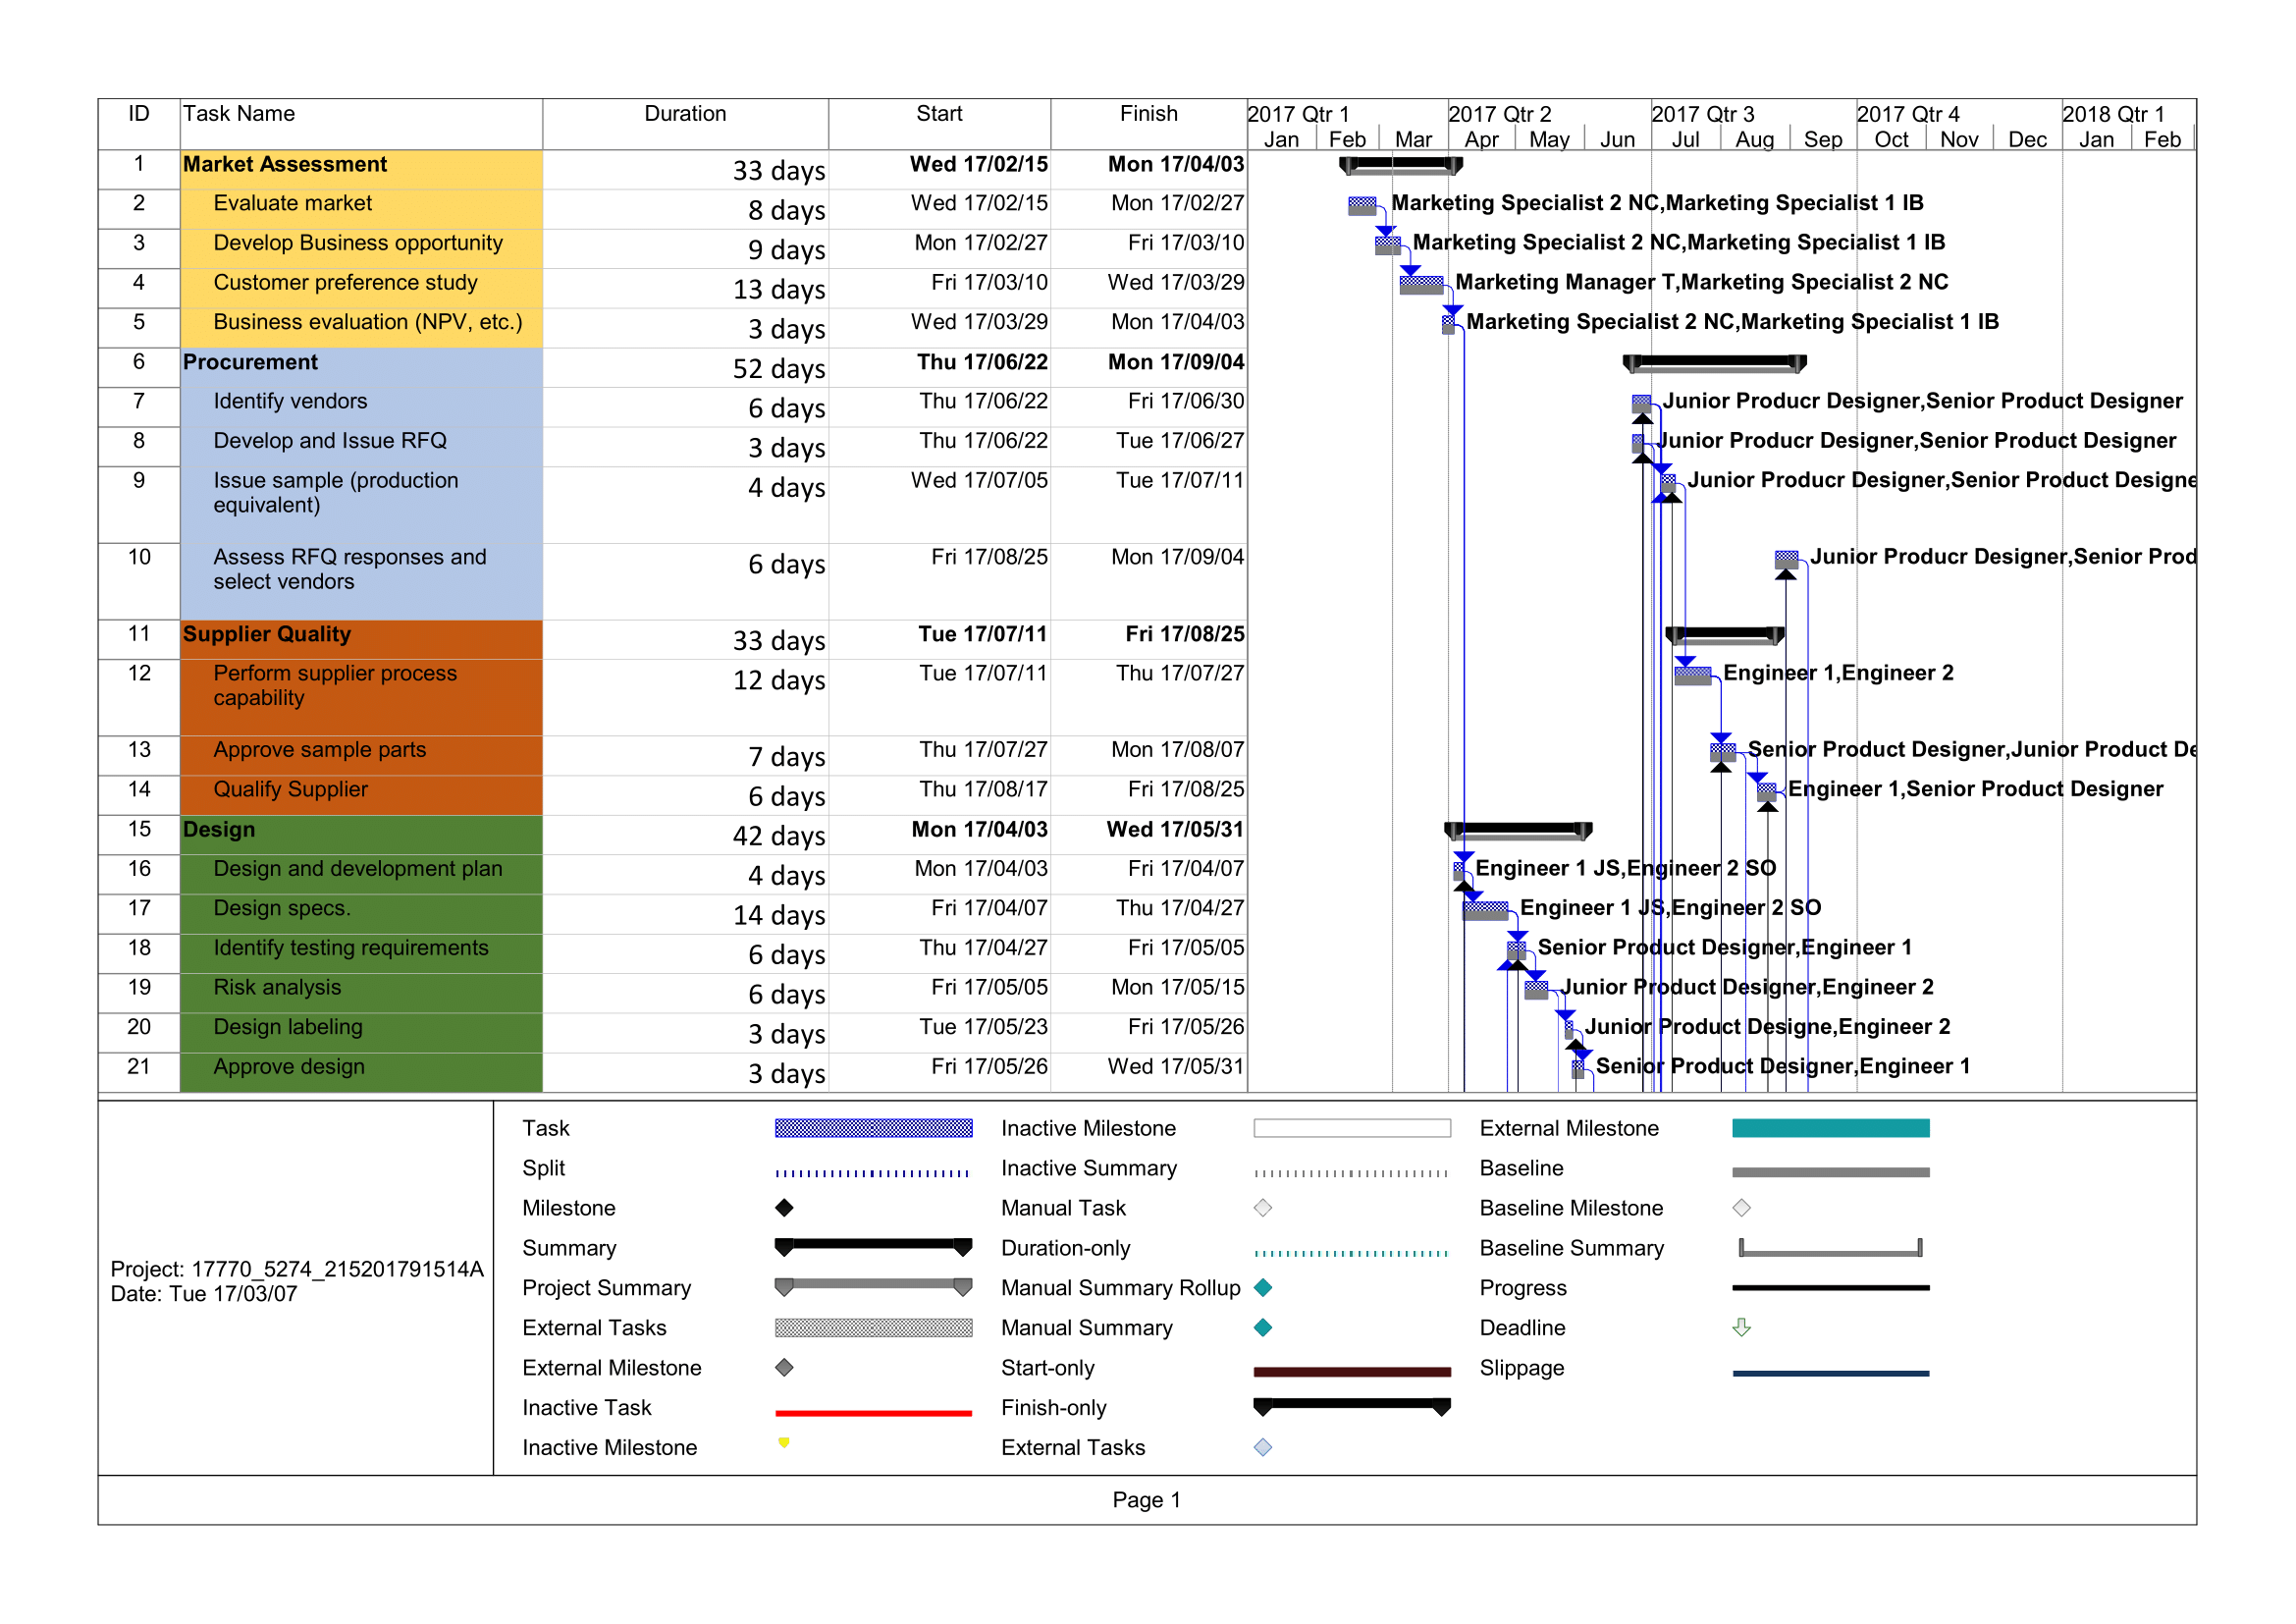
\includegraphics[scale=0.253]{baseline/baseline2-1.png}
\caption{Baseline Part 1}
\end{figure}
\begin{figure}[H]
\centering
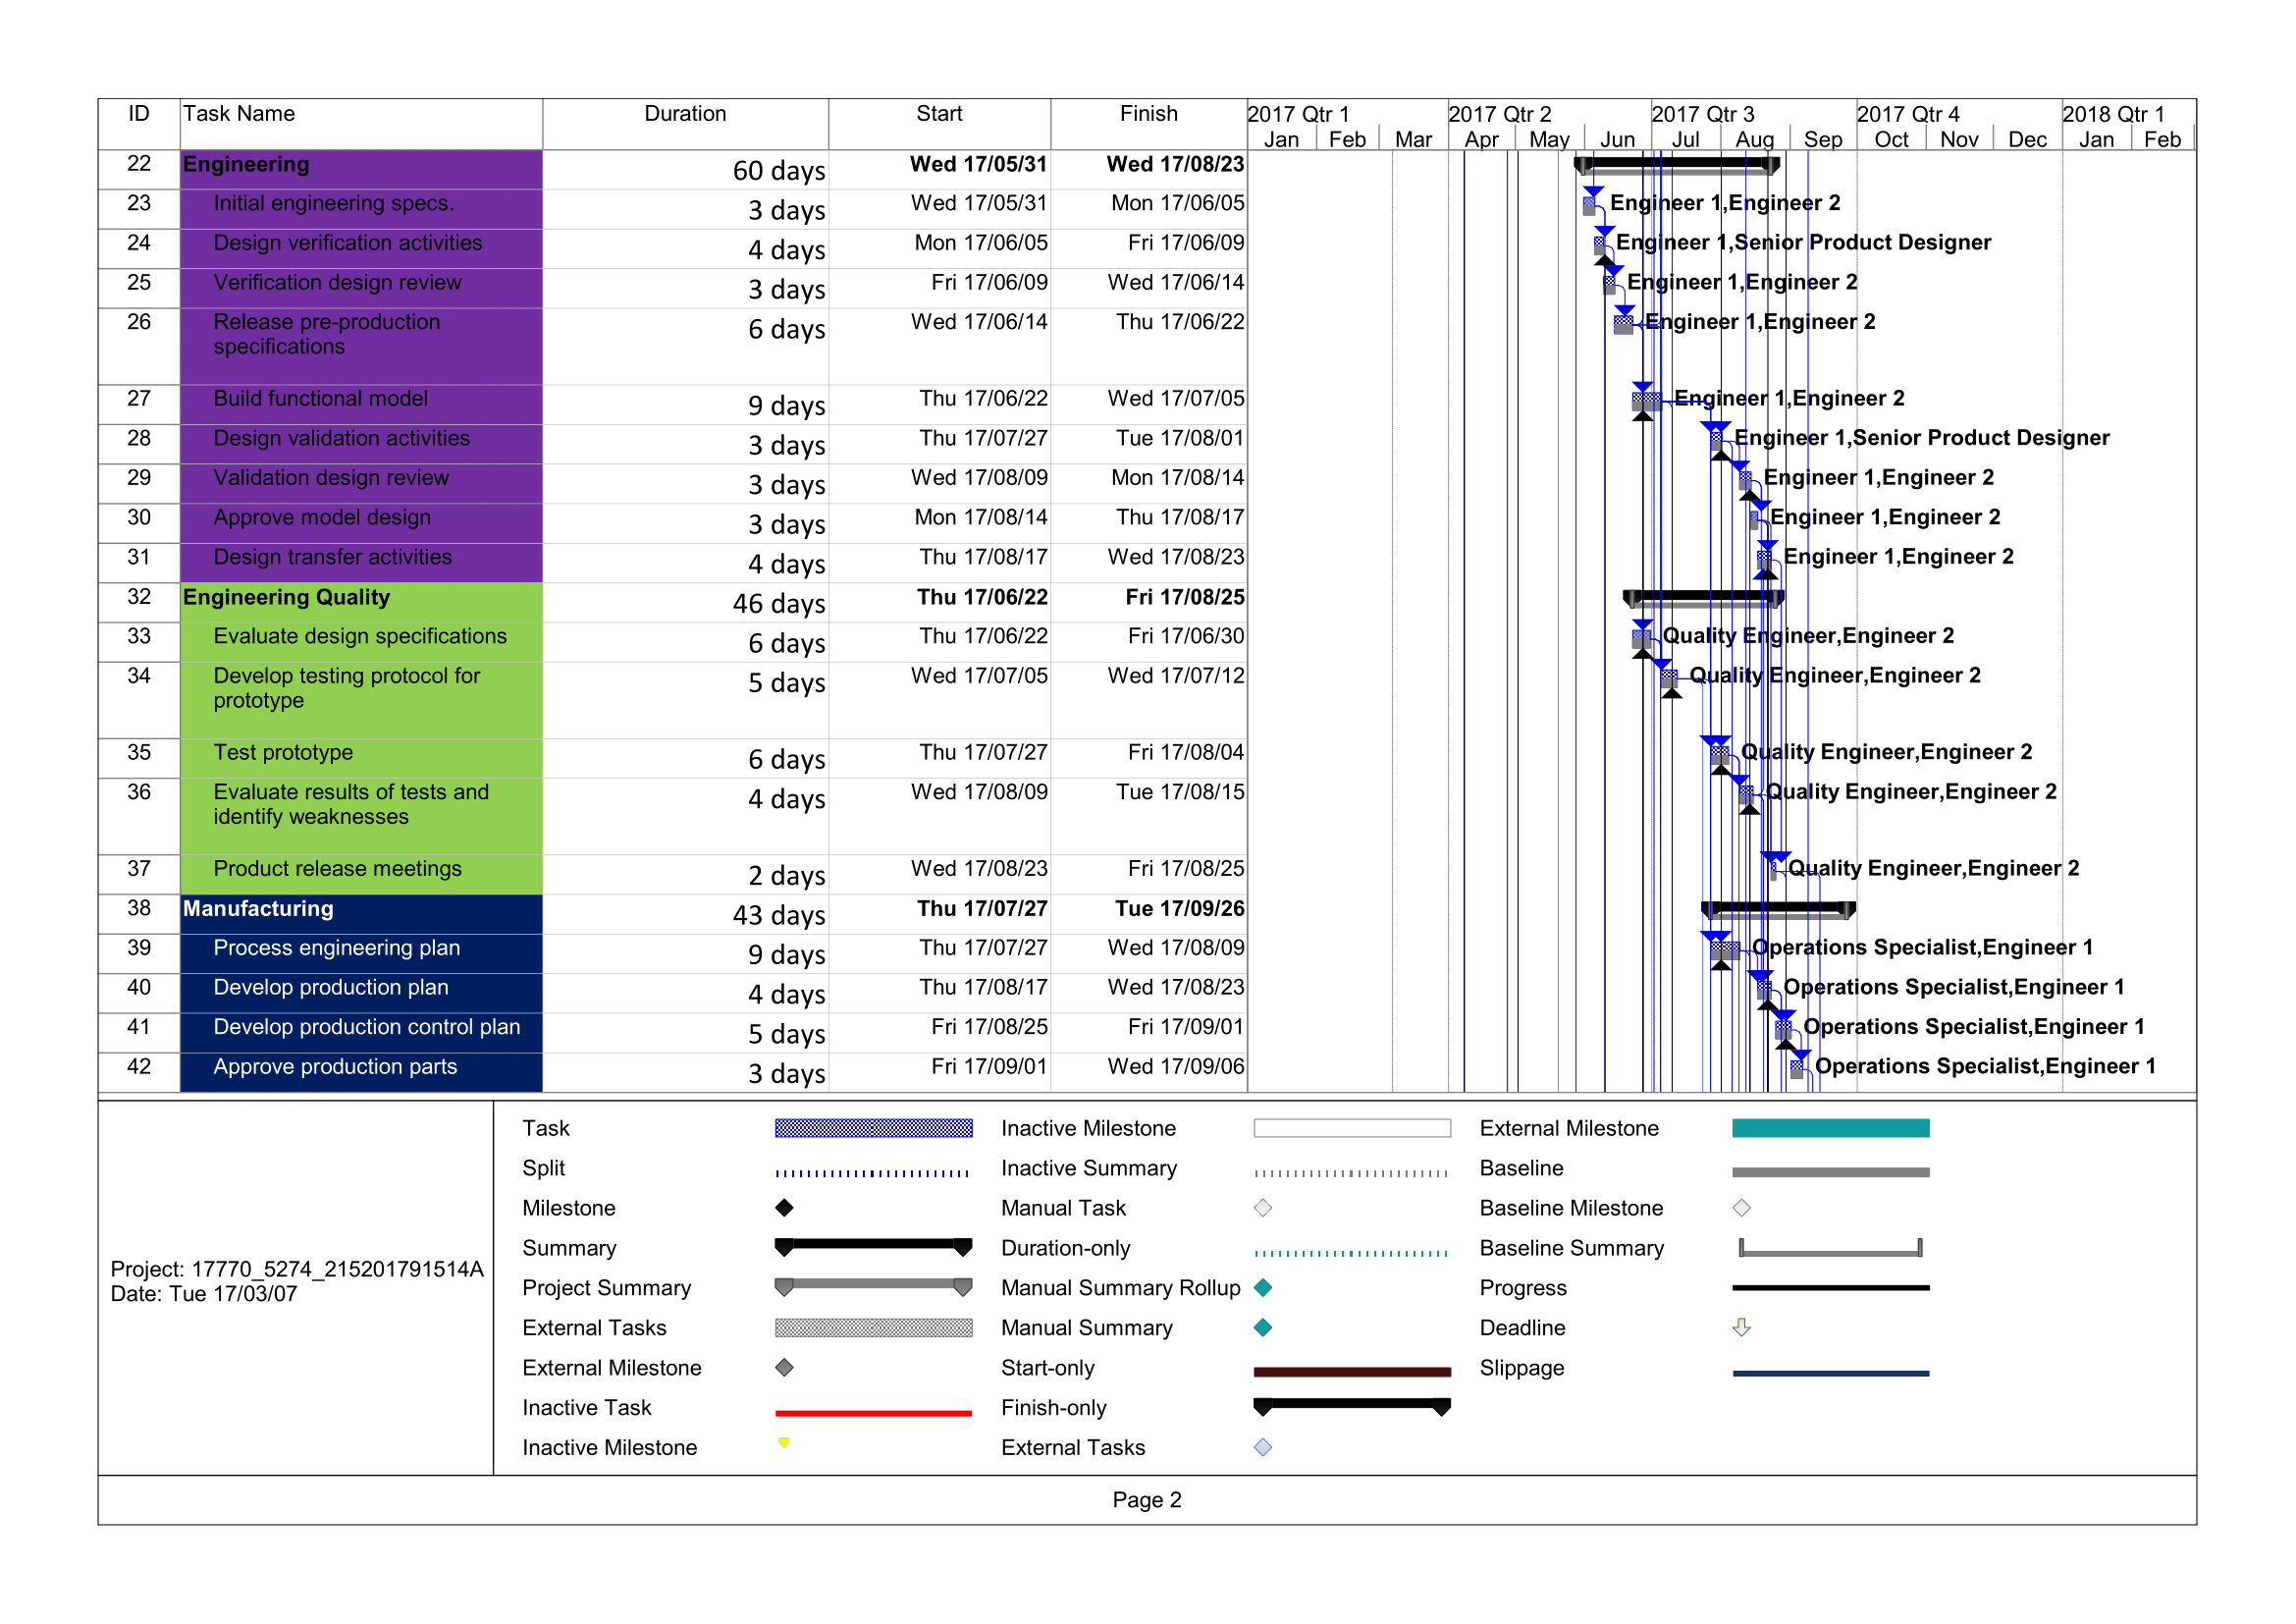
\includegraphics[scale=0.263]{baseline/baseline2-2.png}
\caption{Baseline Part 2}
\end{figure}
\begin{figure}[H]
\centering
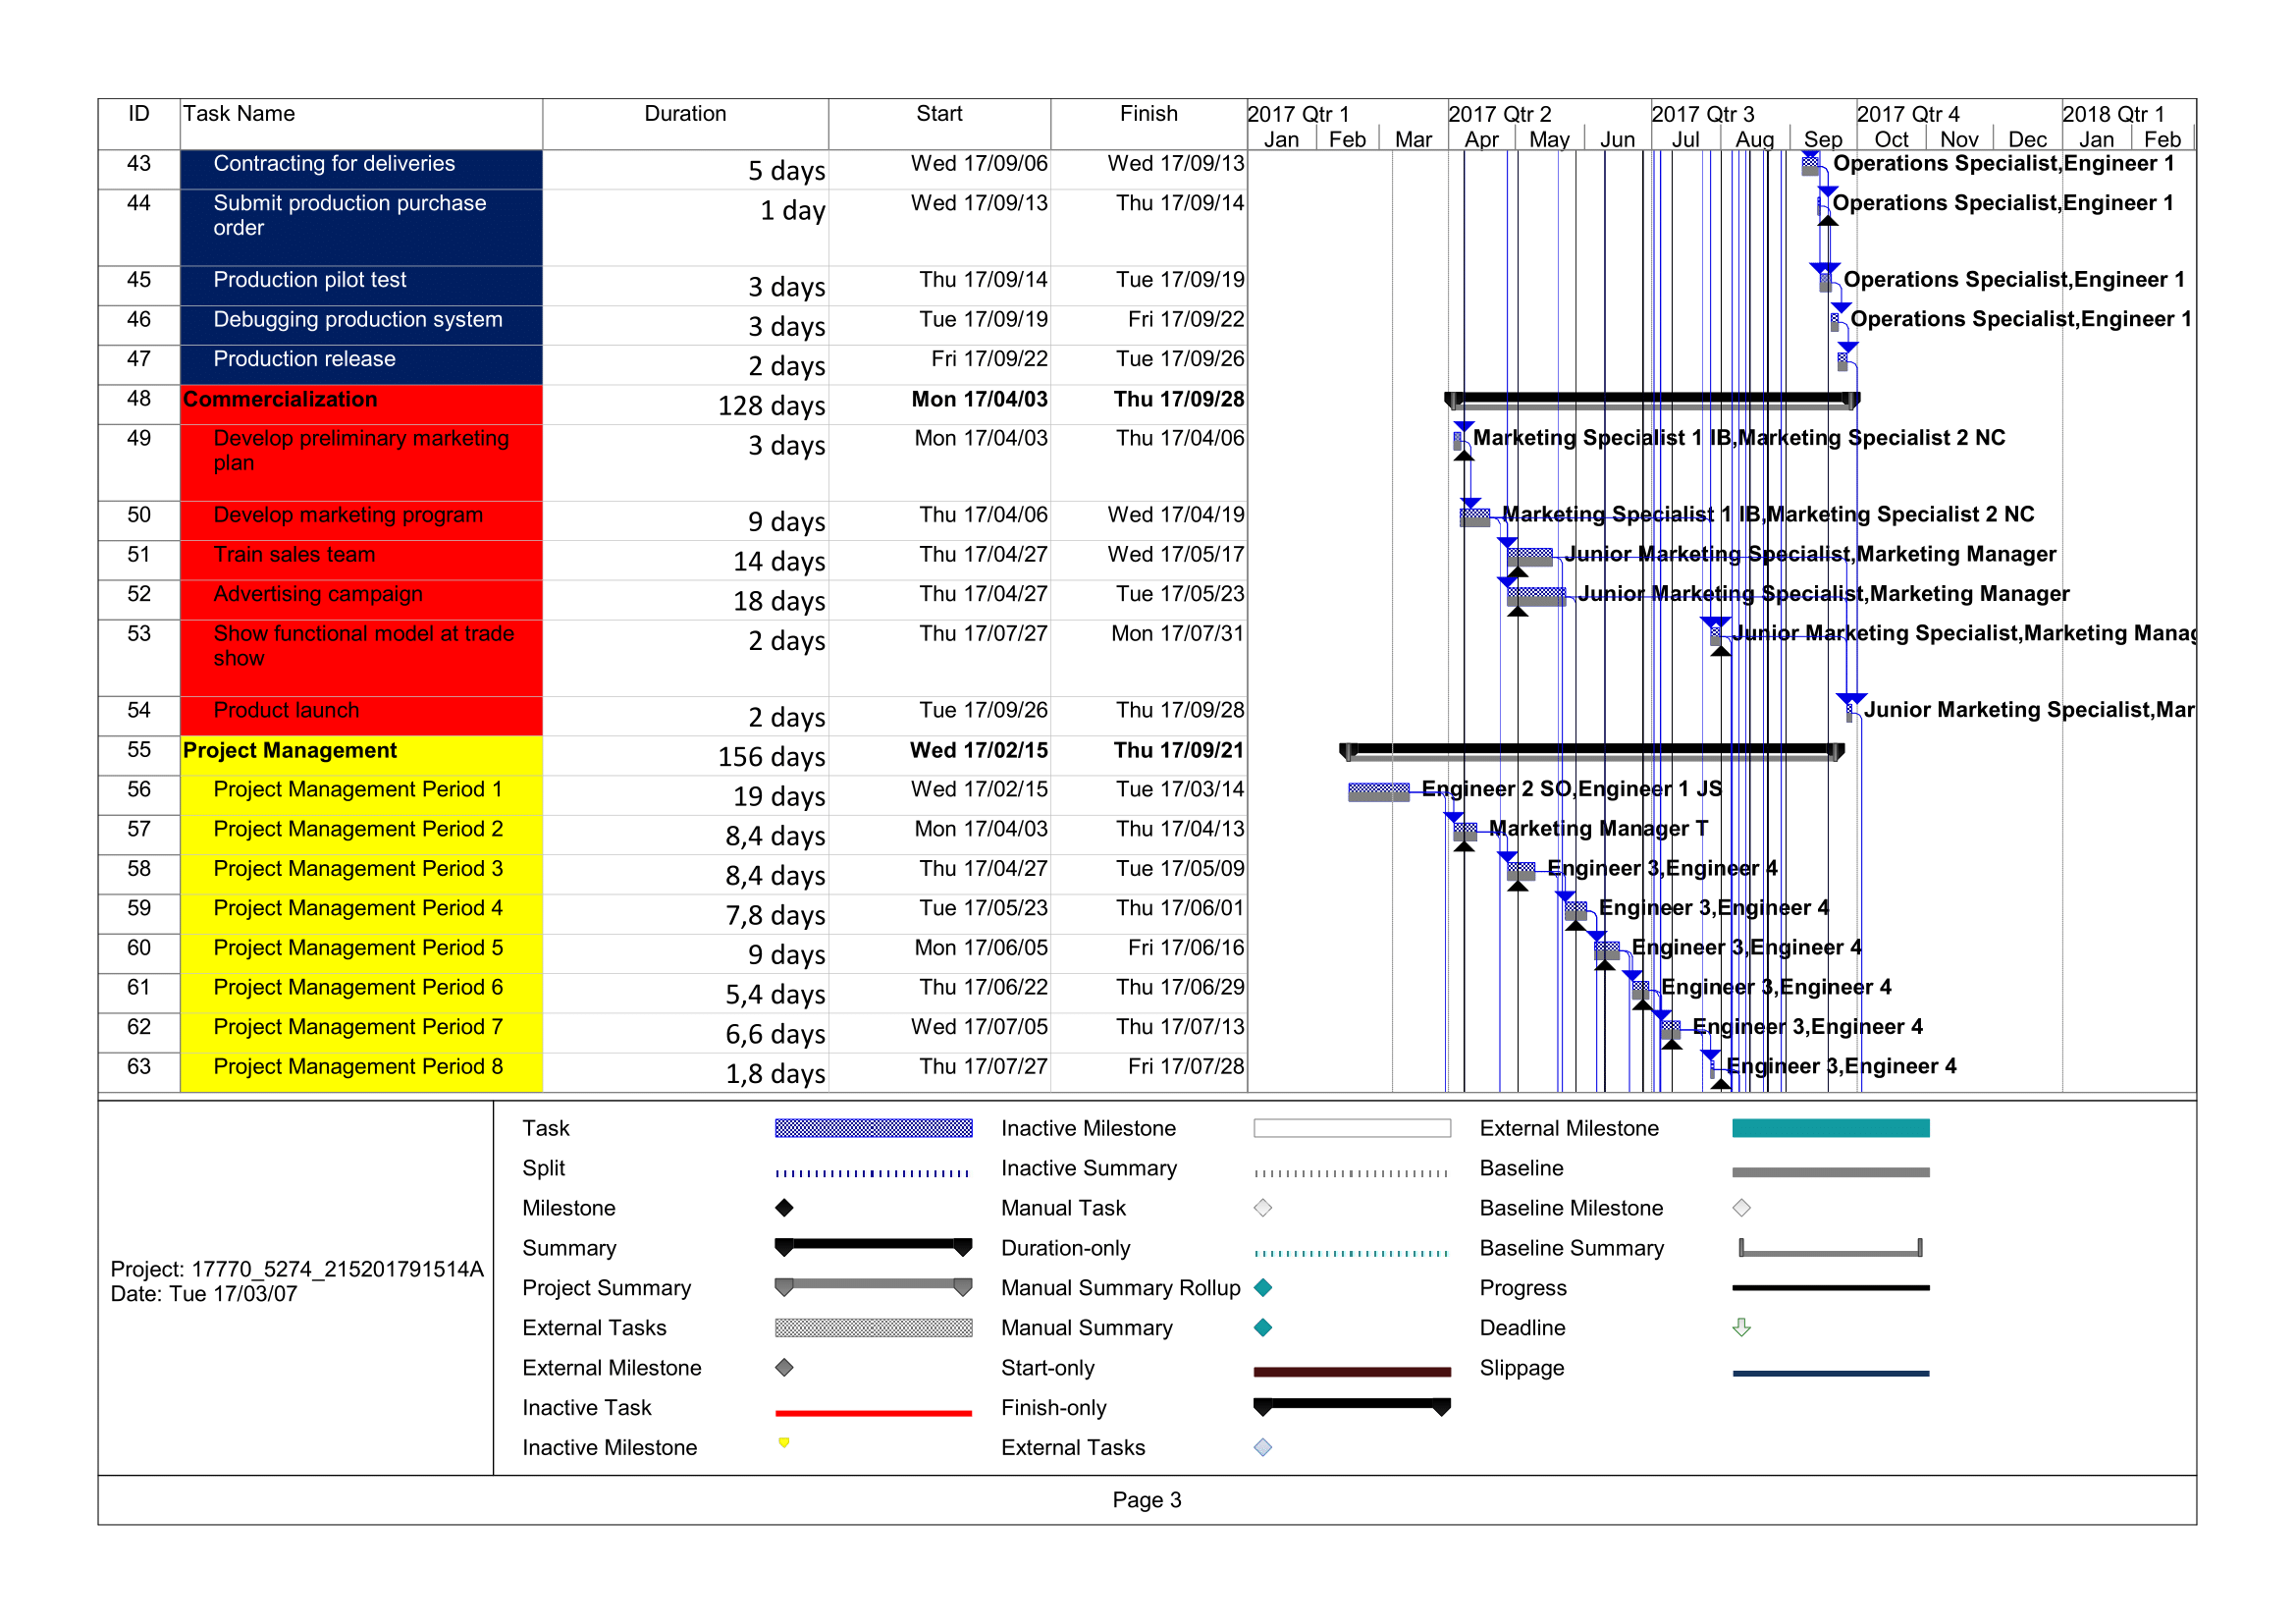
\includegraphics[scale=0.2613]{baseline/baseline2-3.png}
\caption{Baseline Part 3}
\end{figure}
\begin{figure}[H]
\centering
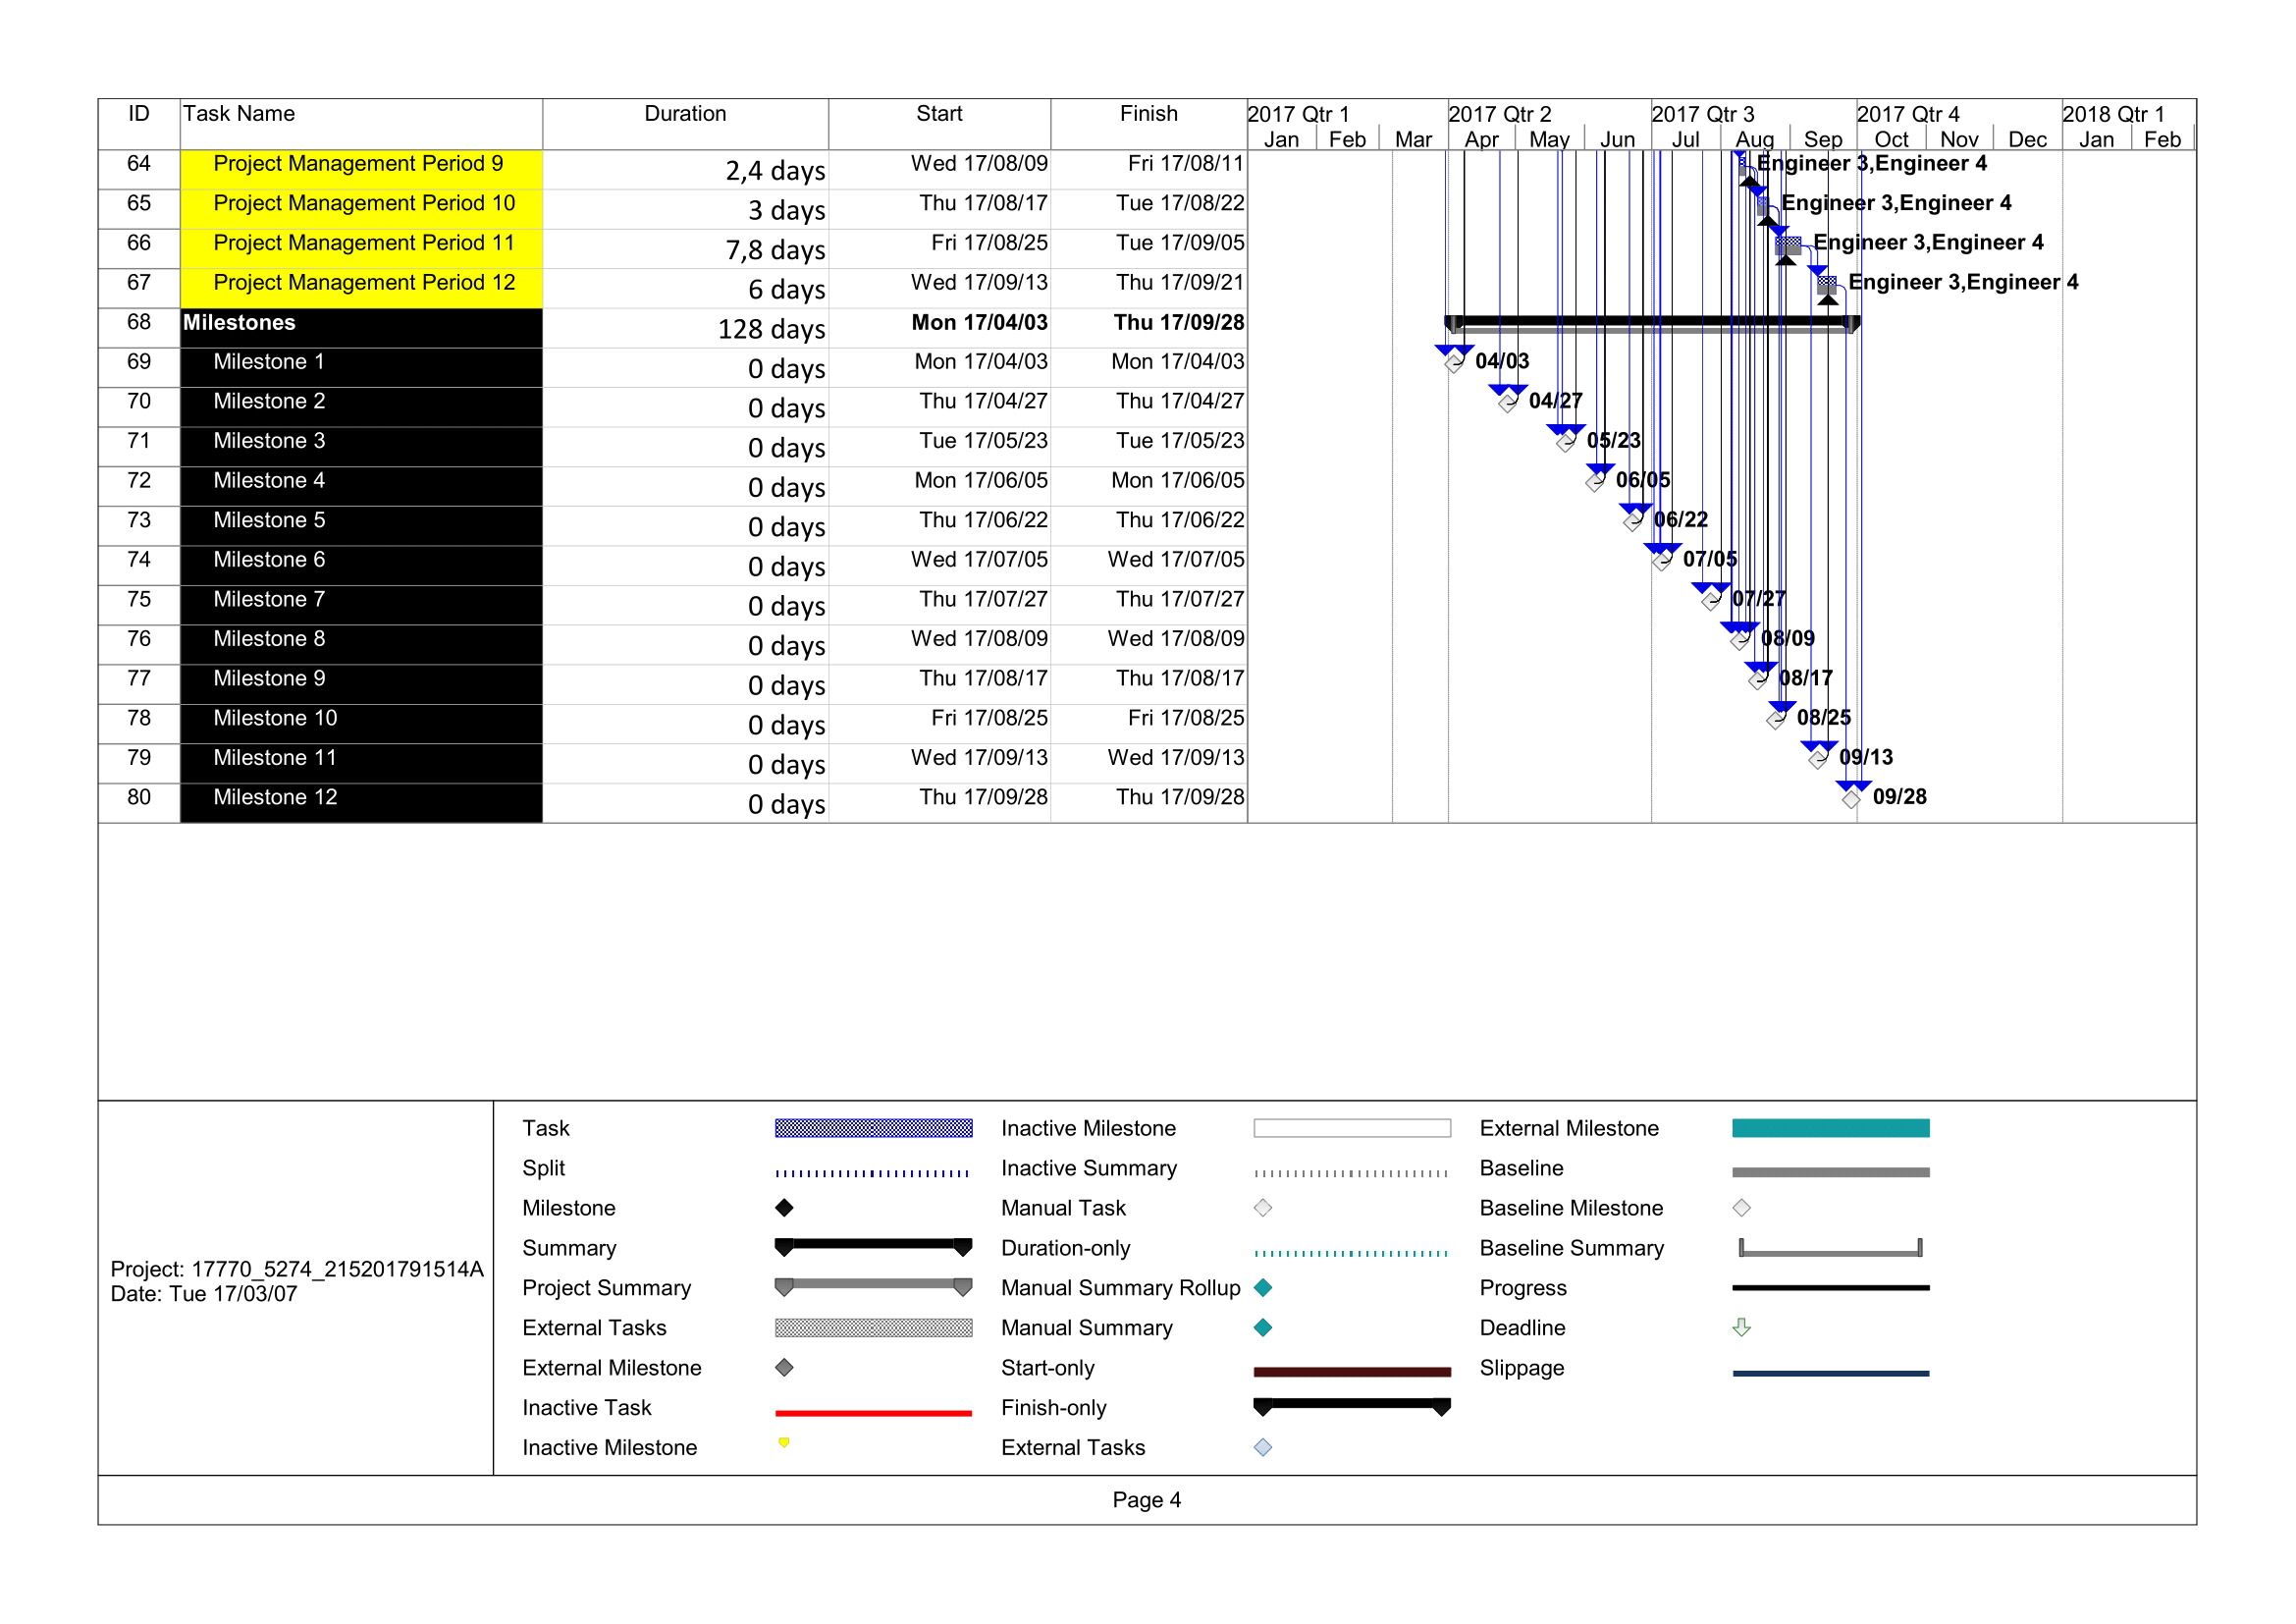
\includegraphics[scale=0.2623]{baseline/baseline2-4.png}
\caption{Baseline Part 4}
\end{figure}
%\begin{figure}[H]
%\centering
%\includegraphics[scale=0.2633]{baseline/baseline-5.png}
%\caption{Baseline Part 5}
%\end{figure}

\end{landscape}

\restoregeometry

\section{Network Diagram}

\begin{figure}[H]
\centering
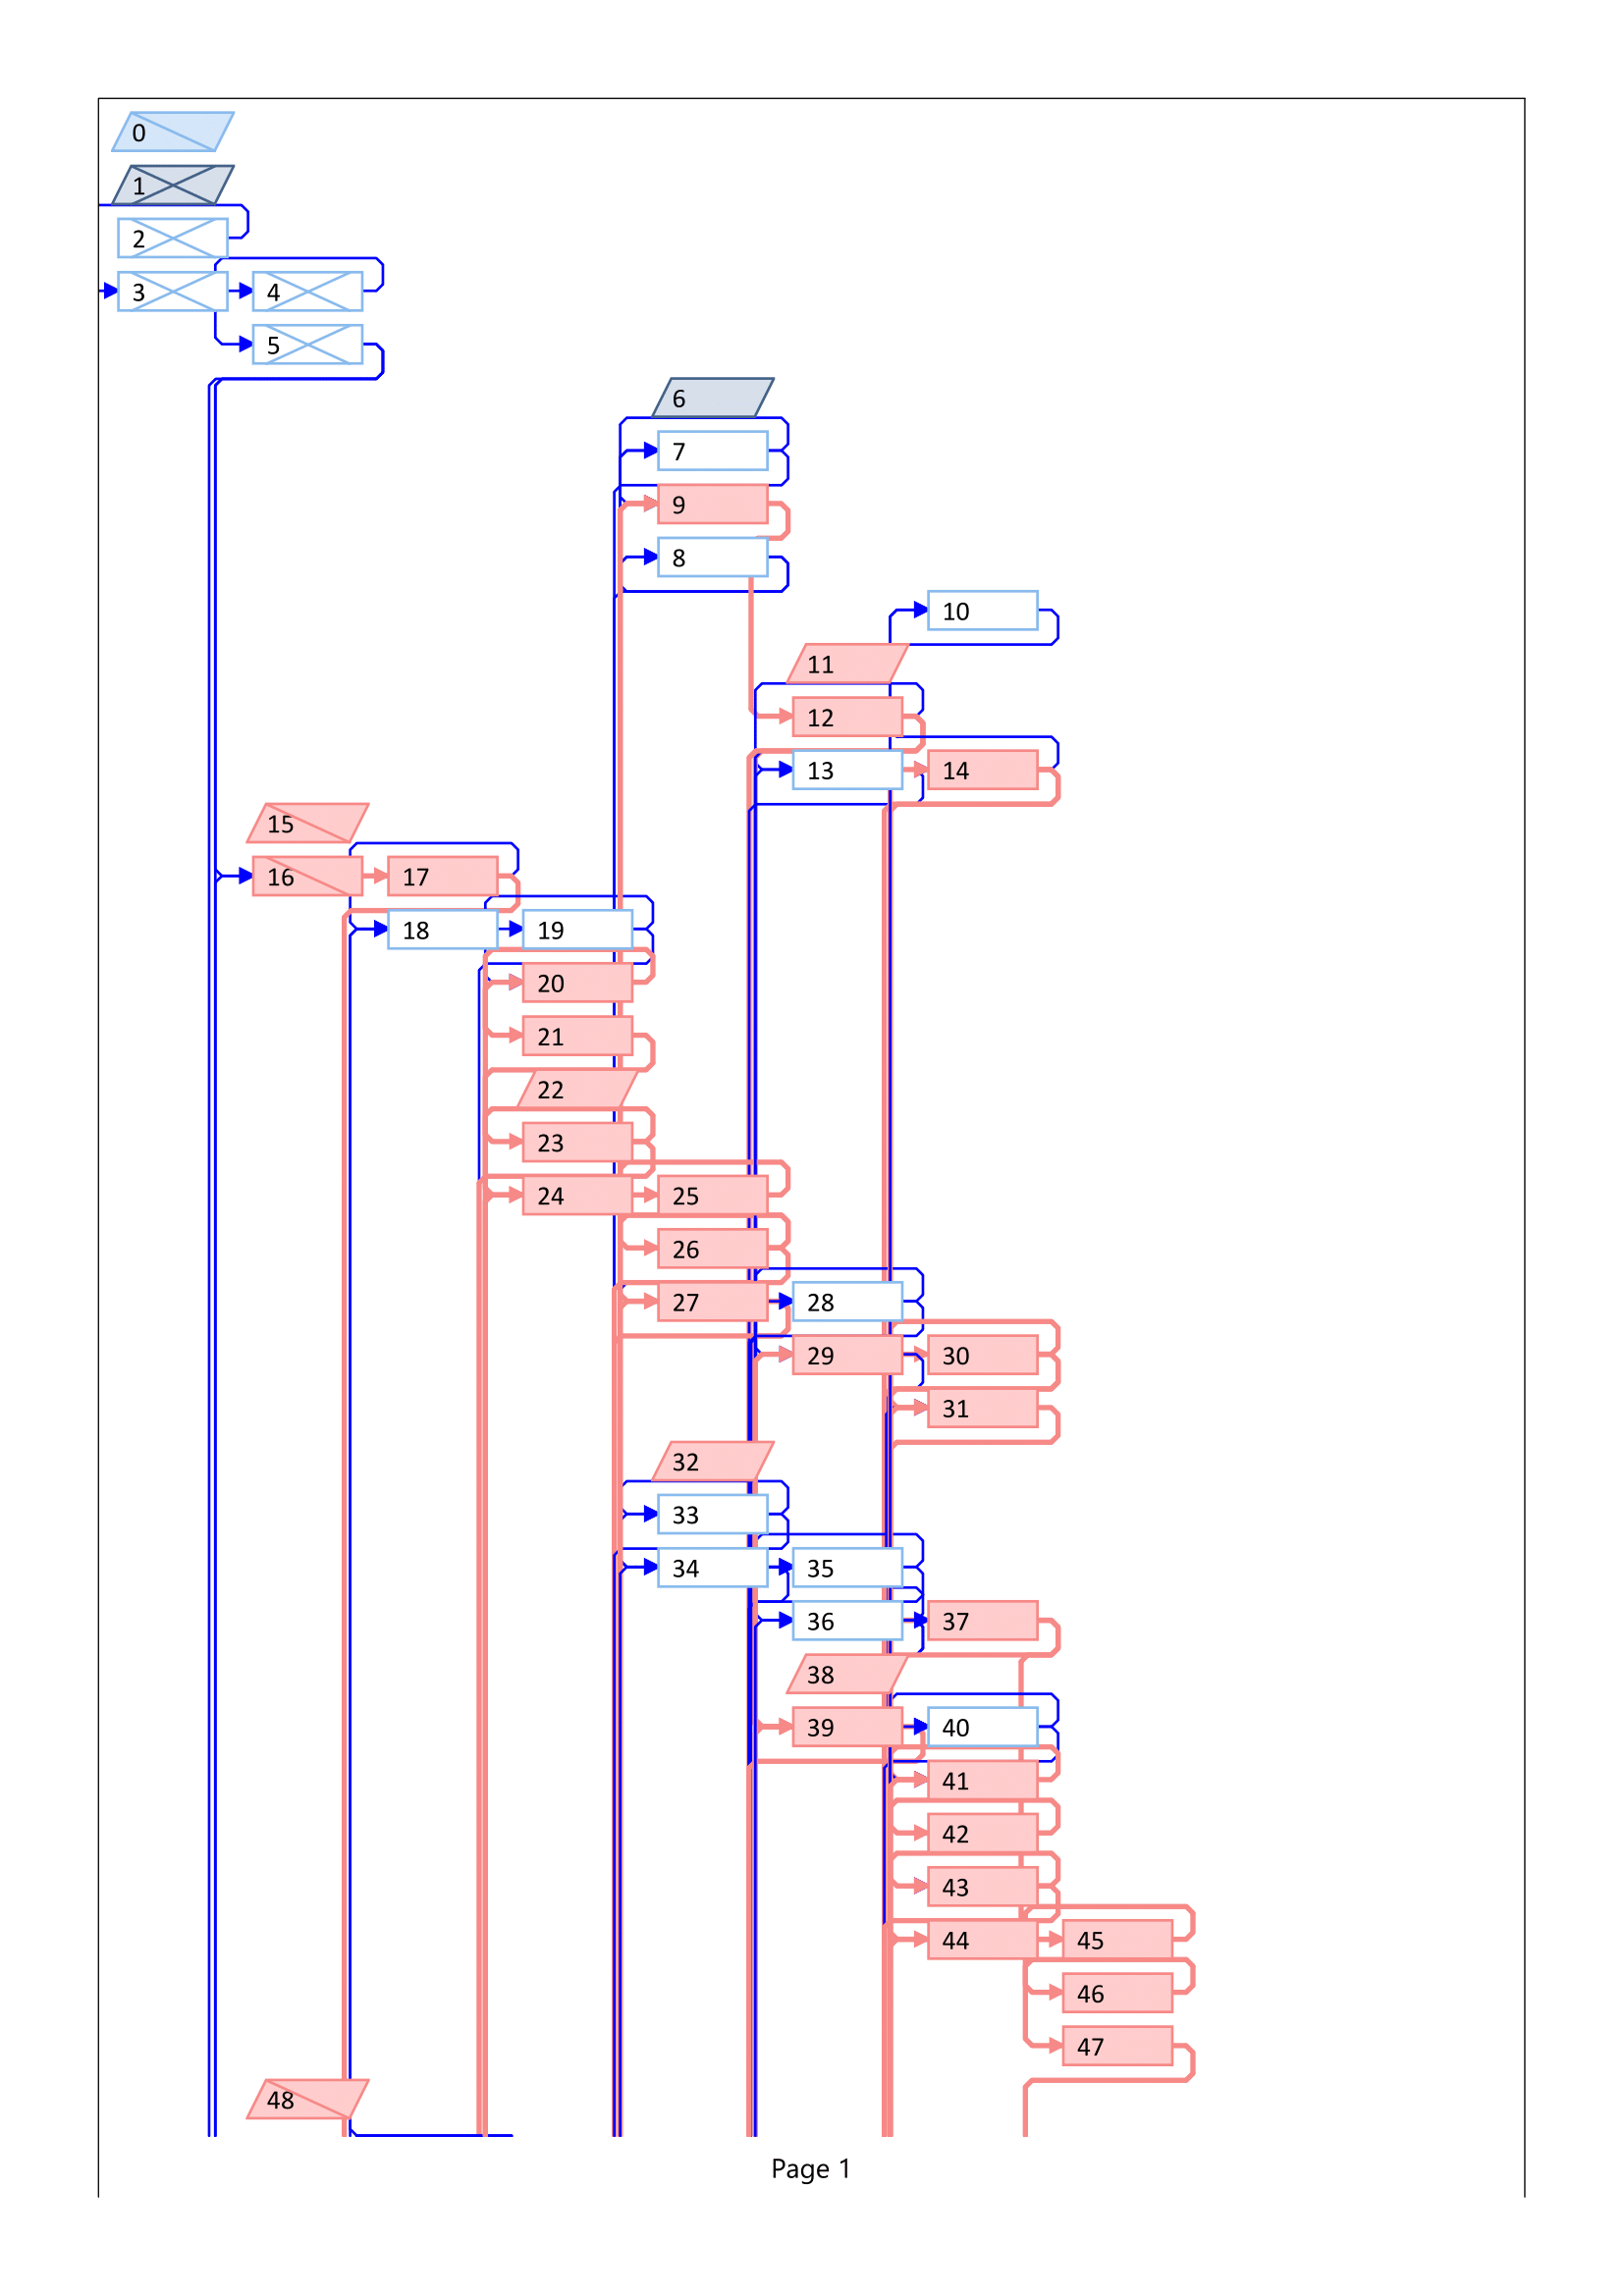
\includegraphics[scale=0.2323]{network_diagram/network_diagram-1.png}
\caption{Network Diagram Part 1}
\end{figure}
\begin{figure}[H]
\centering
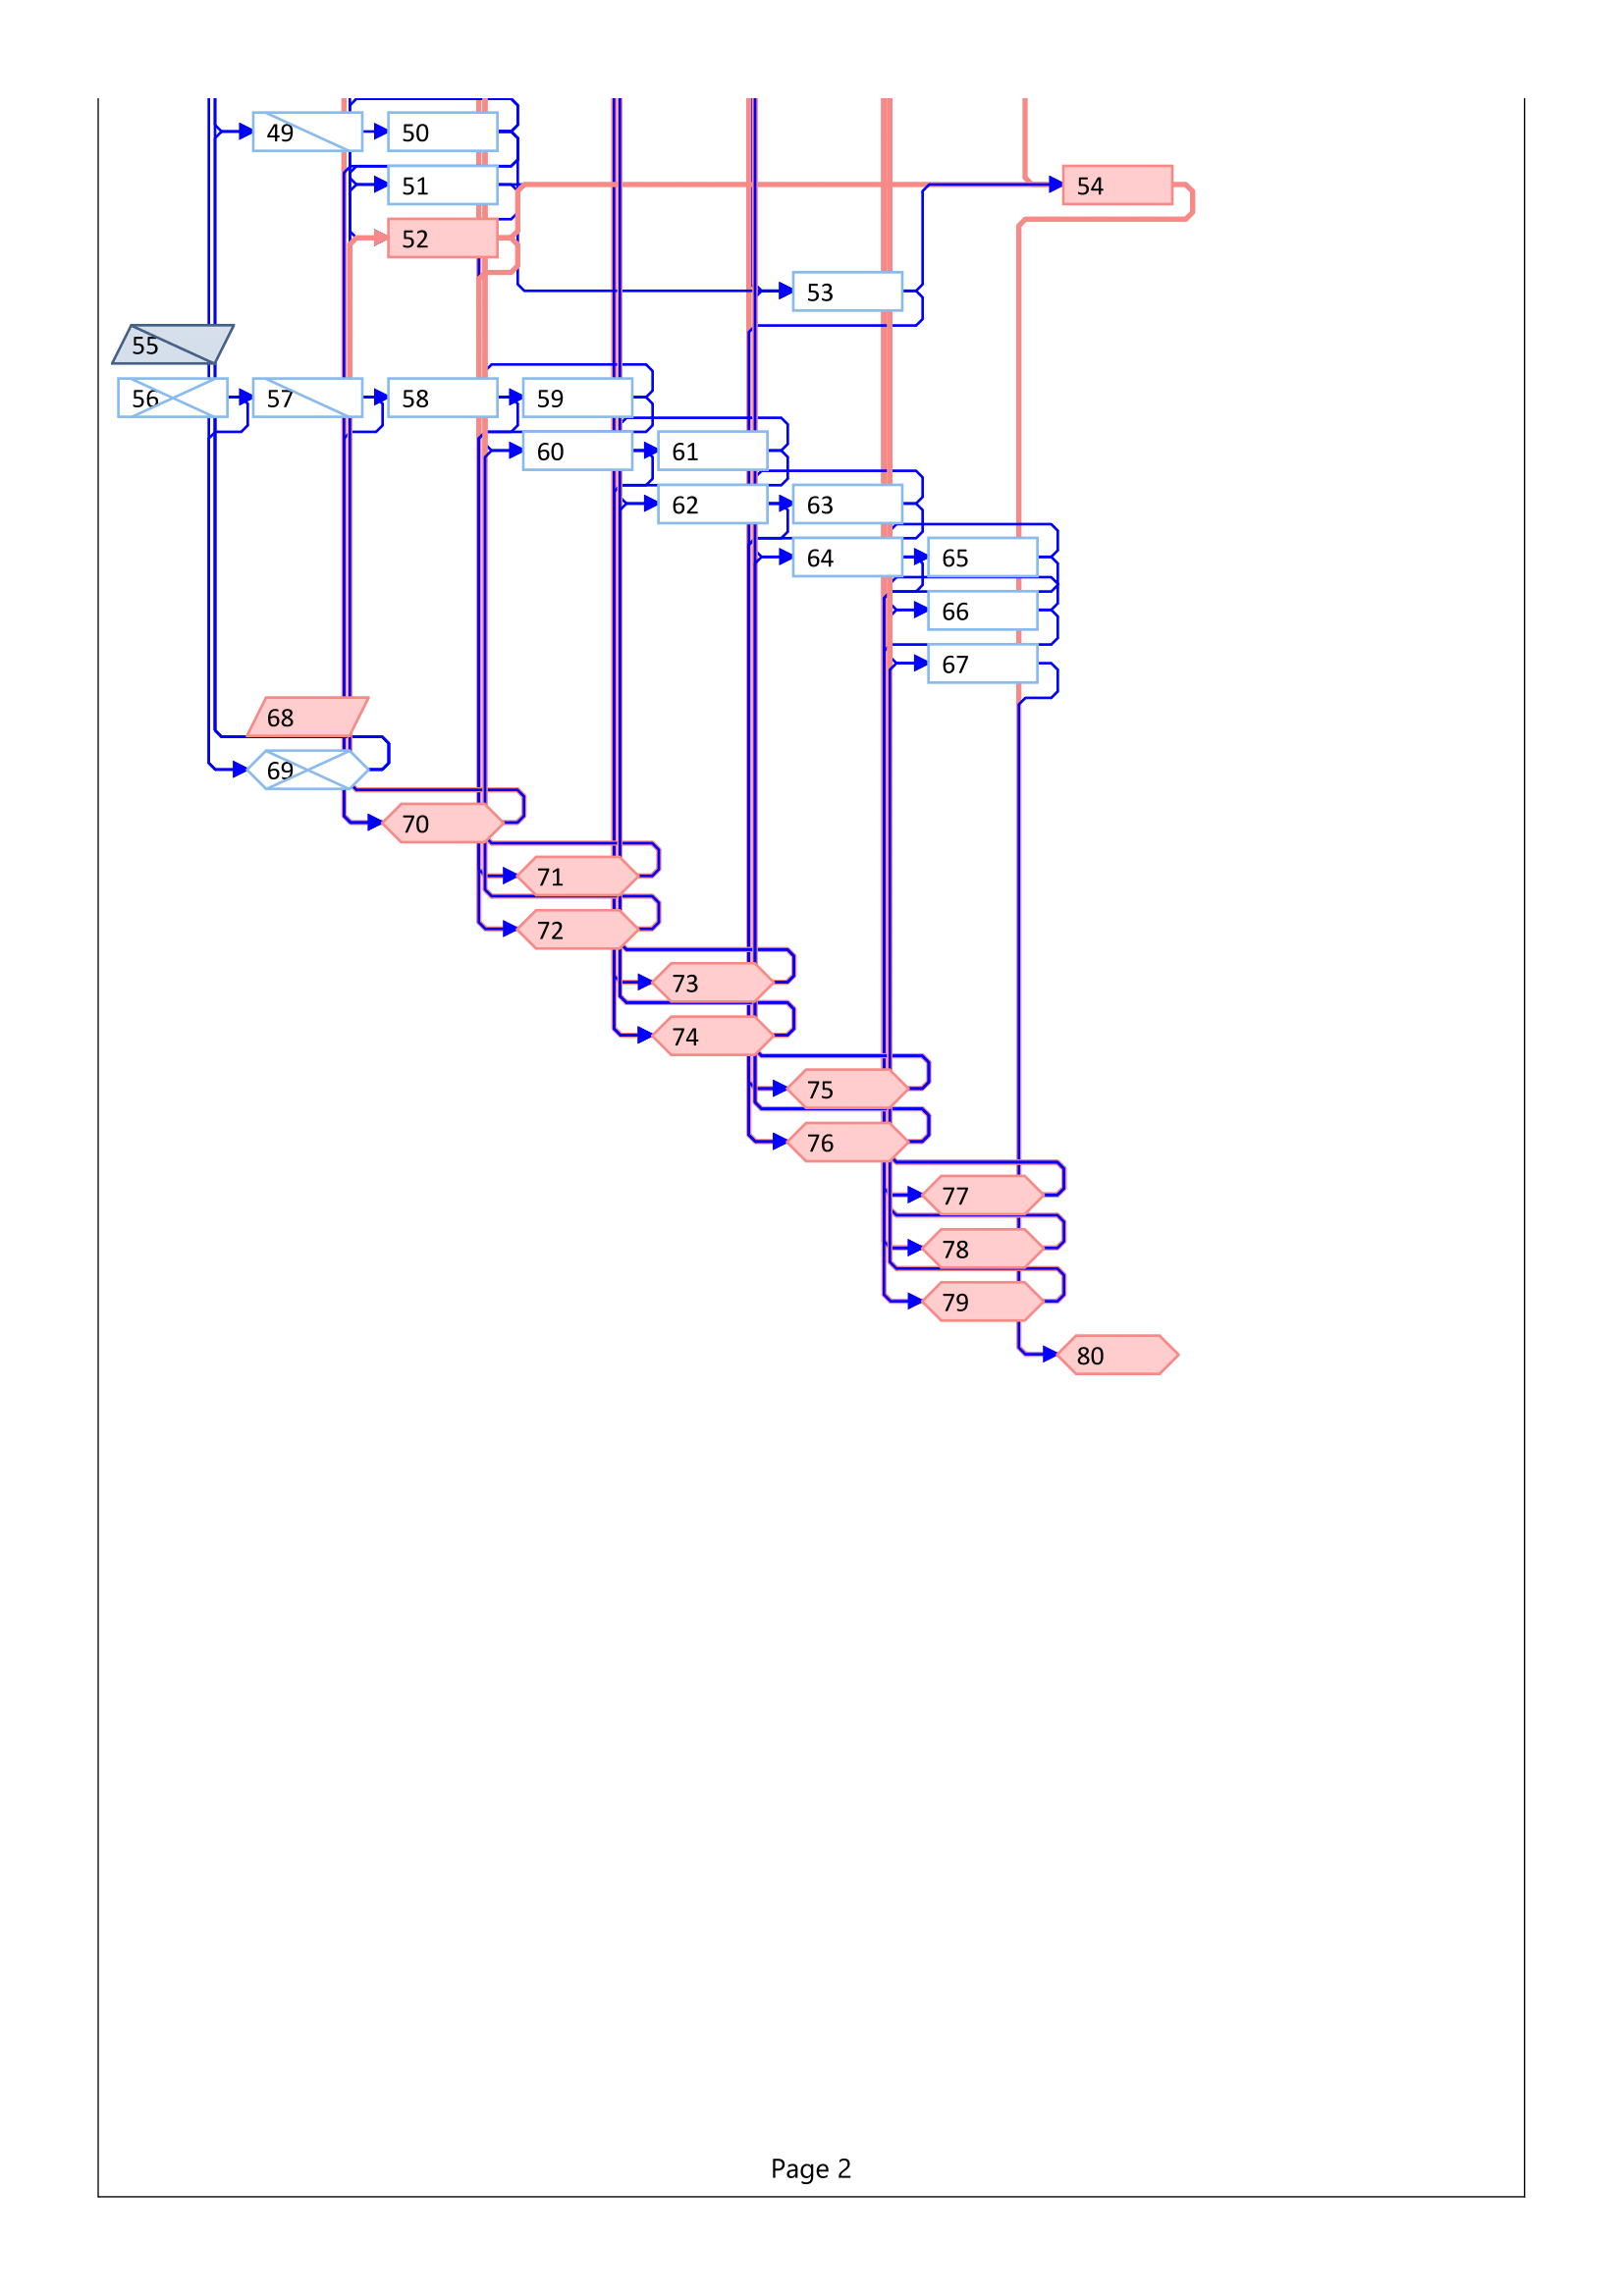
\includegraphics[scale=0.2333]{network_diagram/network_diagram-2.png}
\caption{Network Diagram Part 2}
\end{figure}



% geometry begin
\newgeometry{
 top=2cm,
 bottom=3cm,
 left=2cm,
 right=2cm,
}

\begin{landscape}

\section{Timeline}

\begin{figure}[H]
\centering
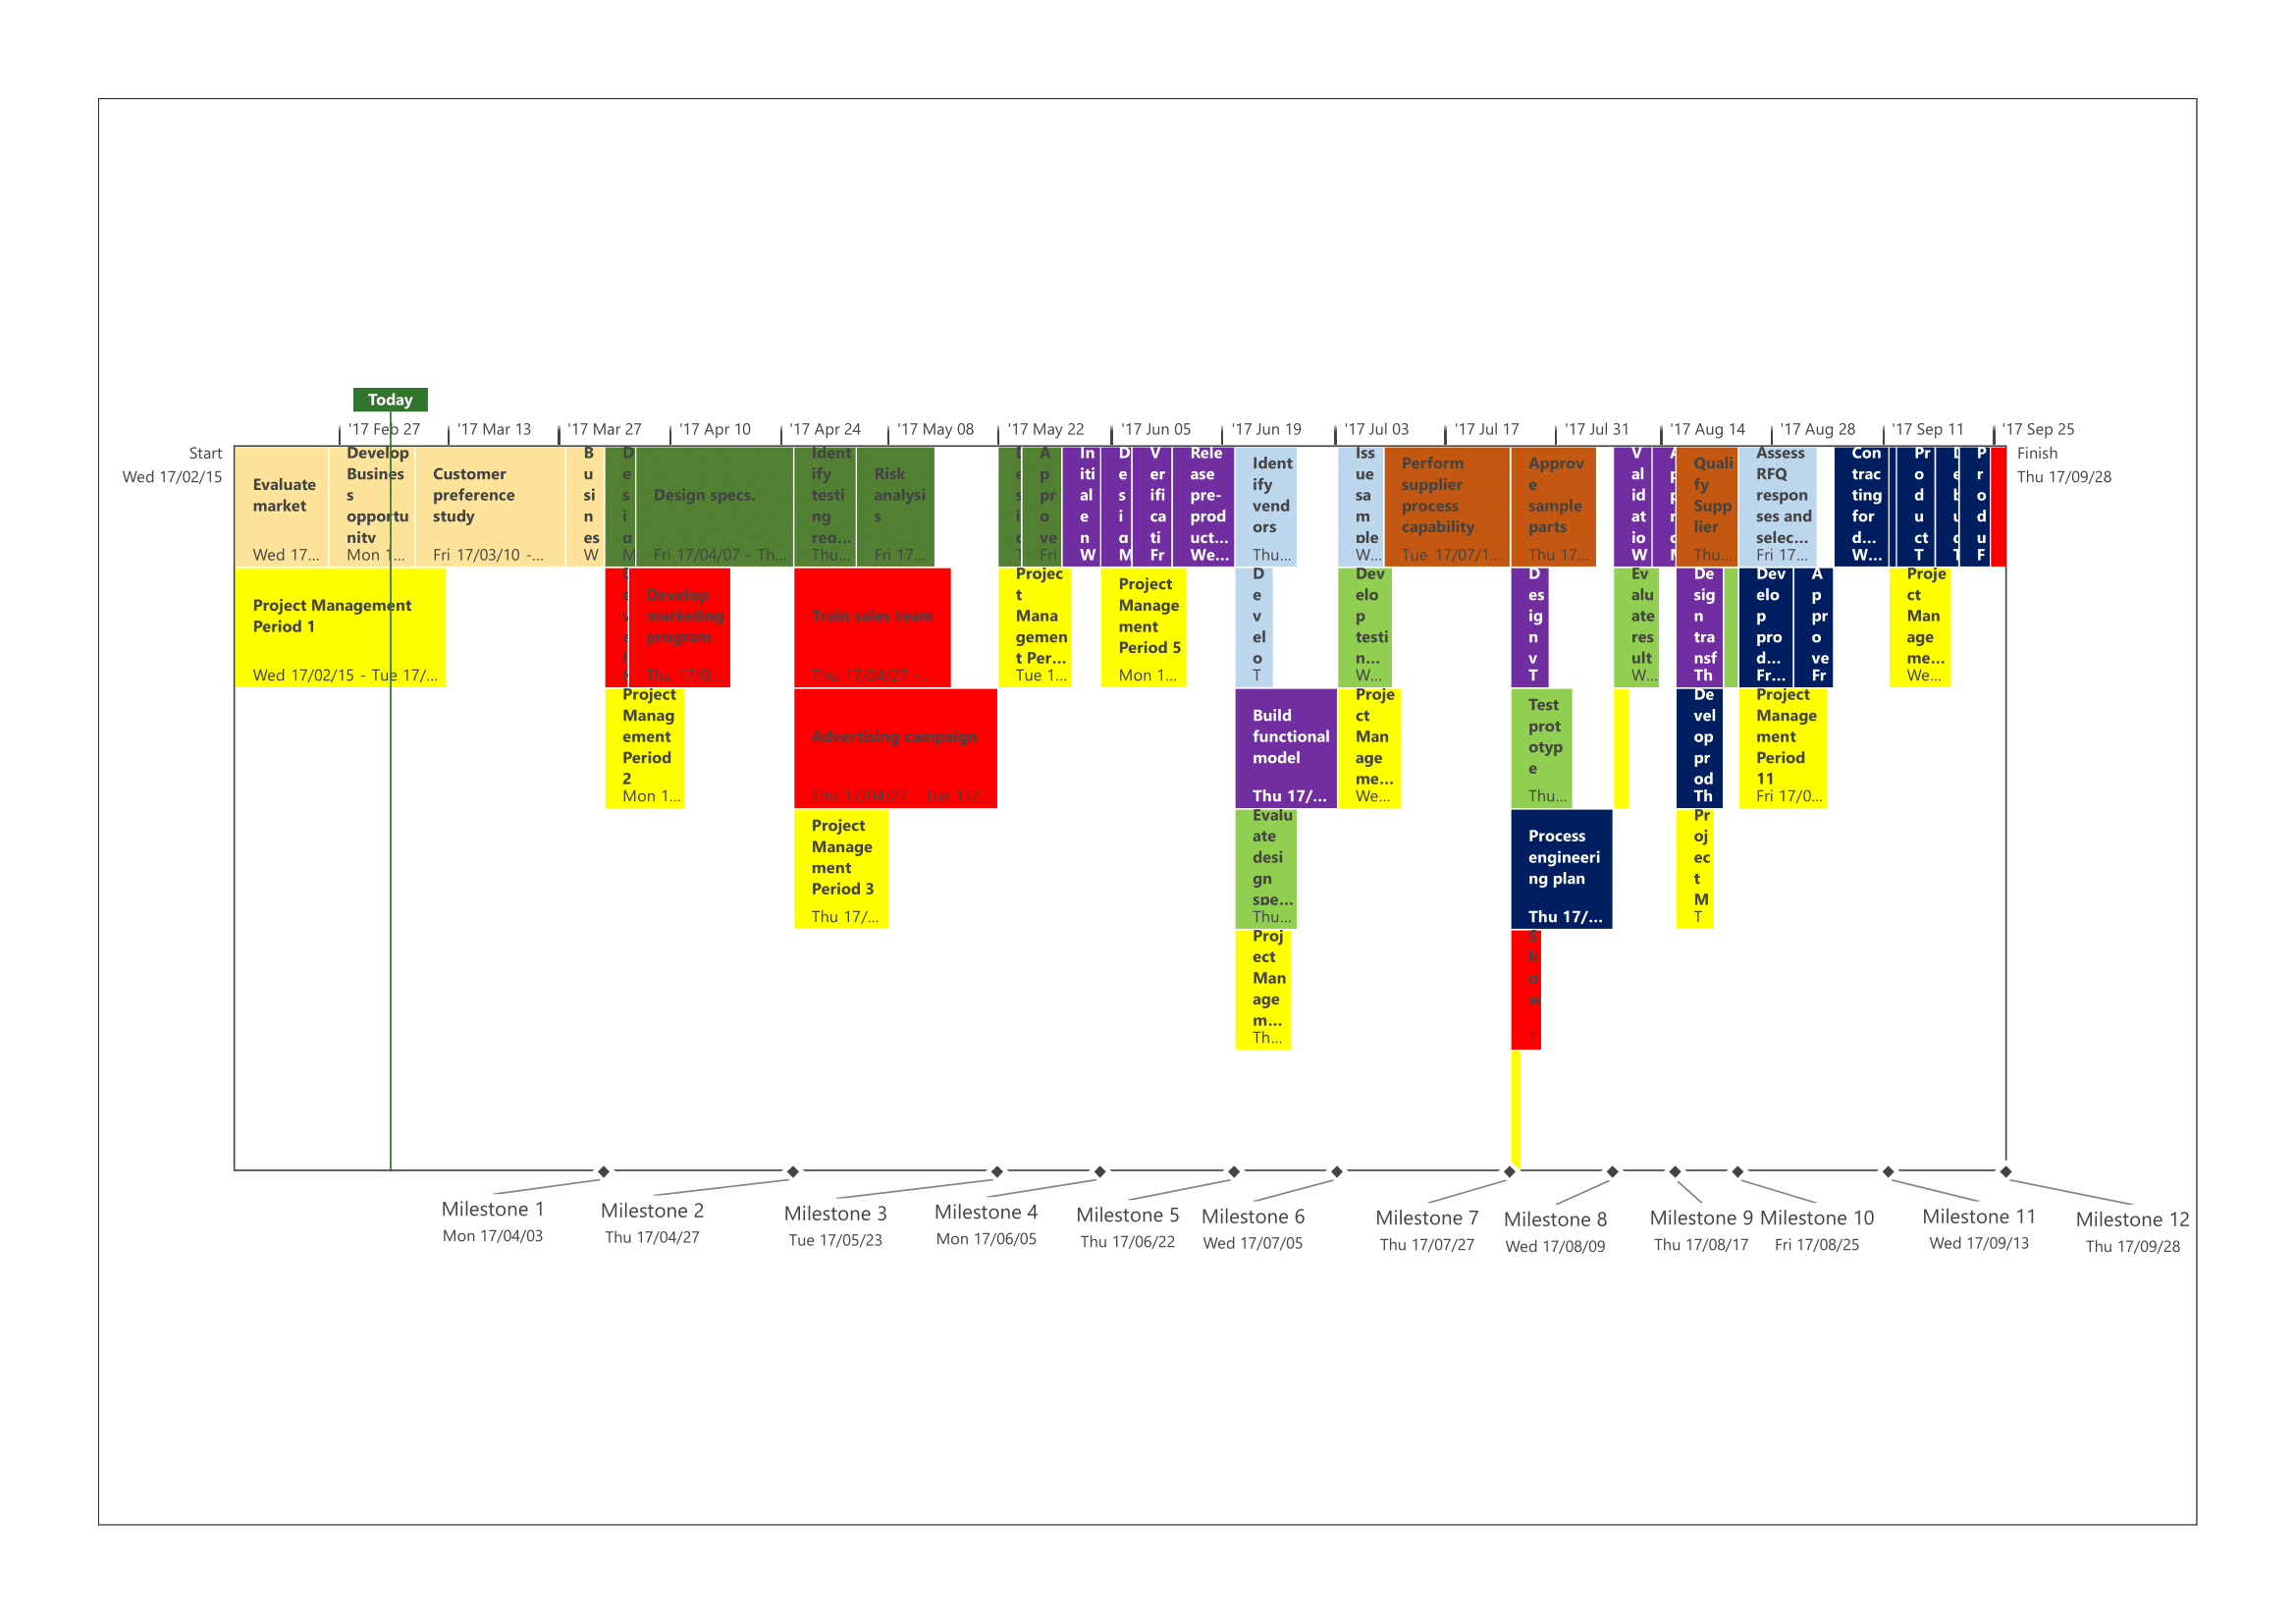
\includegraphics[scale=0.2433]{images/timeline.png}
\caption{Timeline}
\end{figure}

\end{landscape}

\restoregeometry

\section{Meeting Minutes}
\label{appendix:minutes}

\begin{figure}[H]
\centering
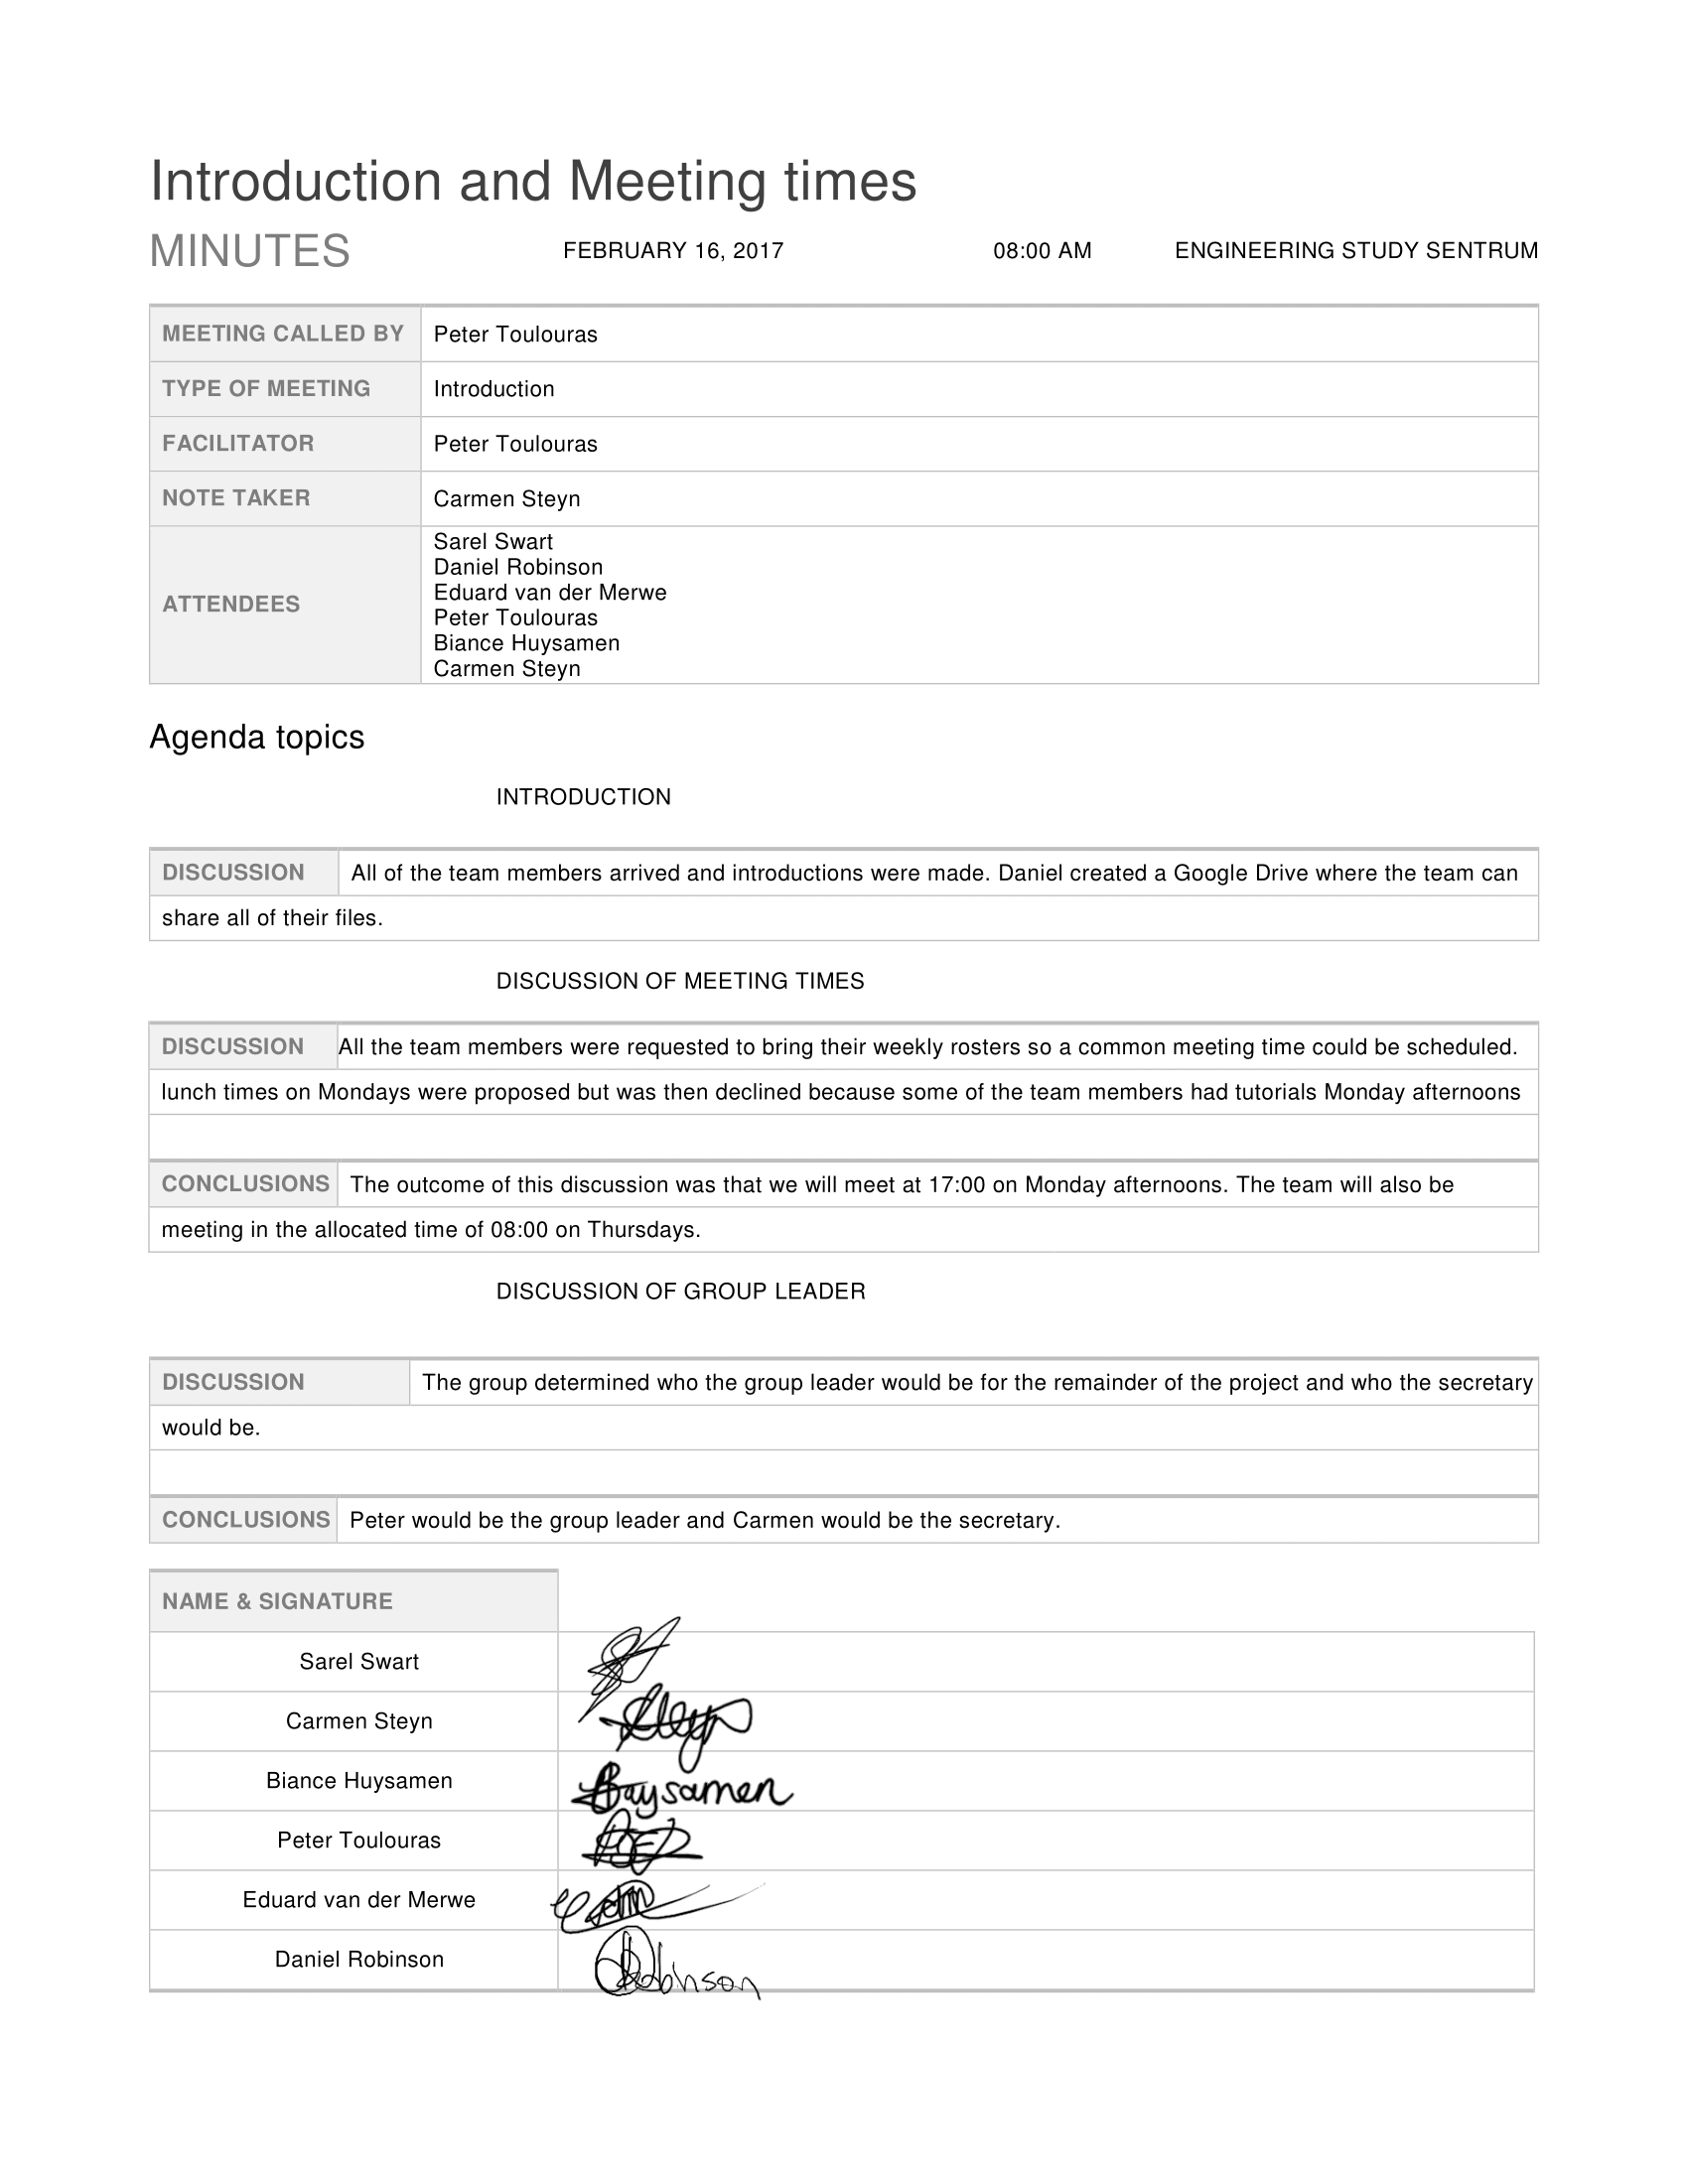
\includegraphics[scale=0.25]{Meeting_minutes_16_Feb.png}
\caption{Minutes 16 Feb}
\end{figure}

\begin{figure}[H]
\centering
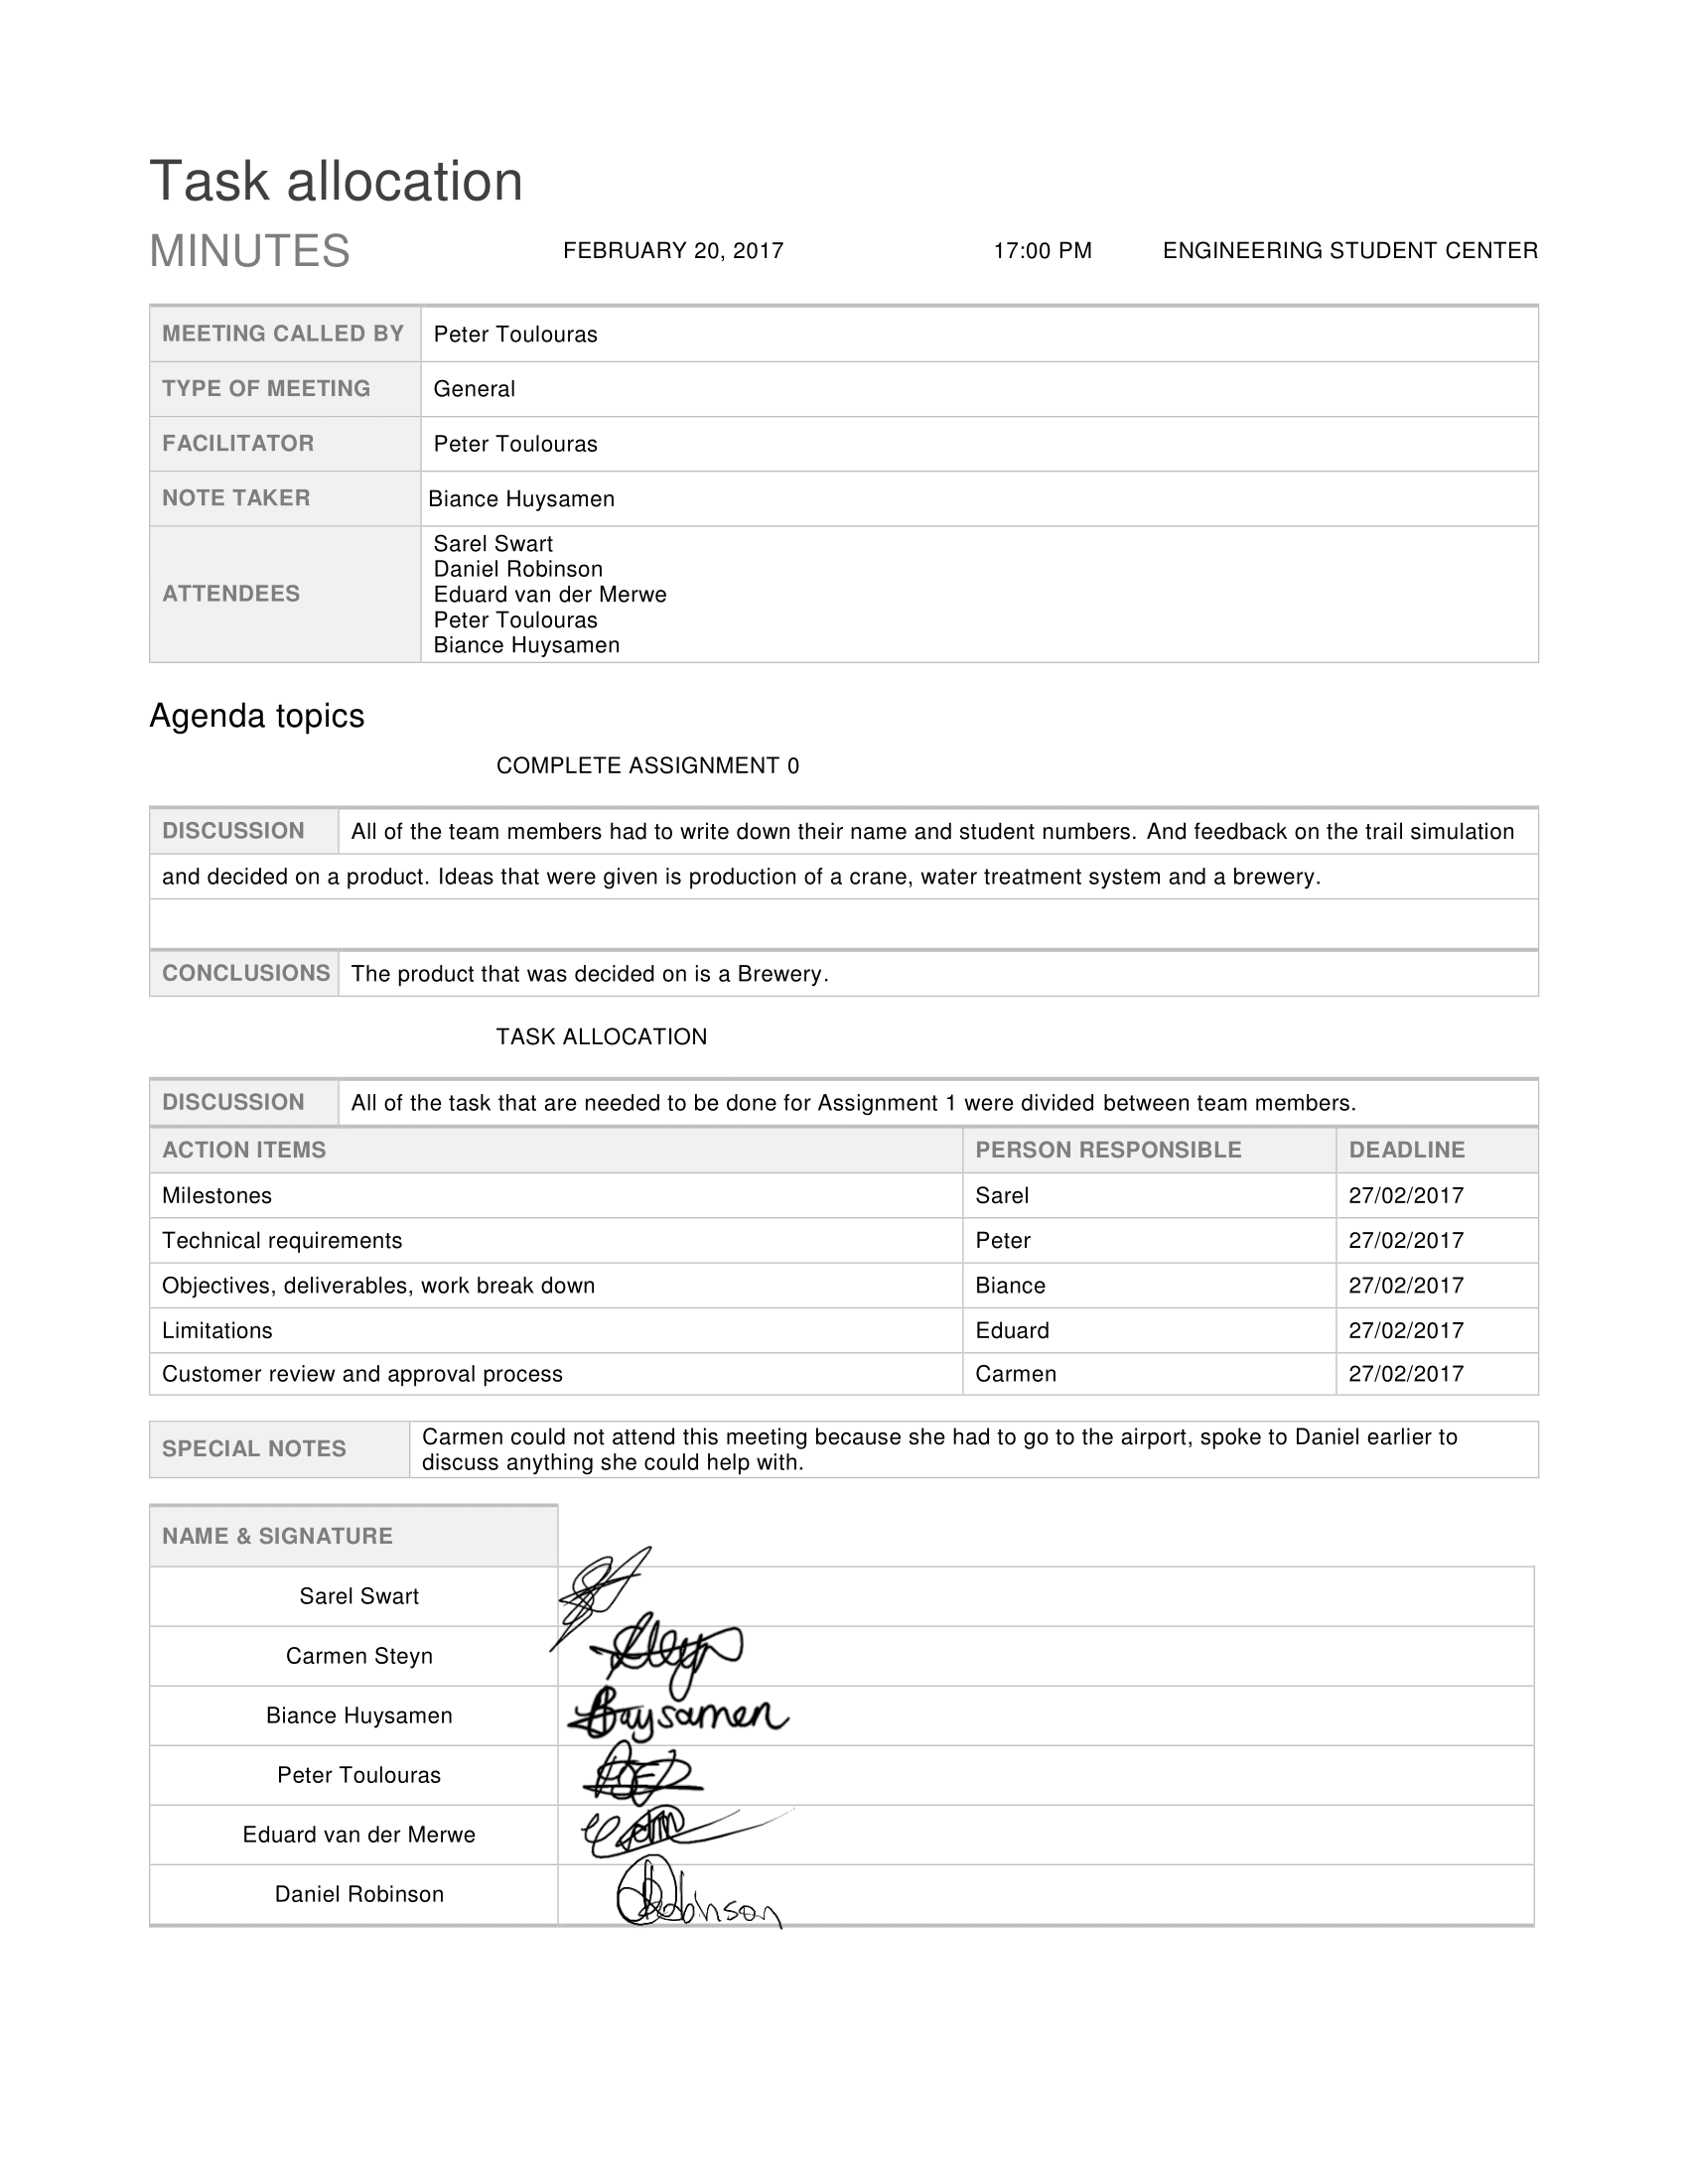
\includegraphics[scale=0.25]{Meeting_minutes_20_Feb.png}
\caption{Minutes 20 Feb}
\end{figure}

\begin{figure}[H]
\centering
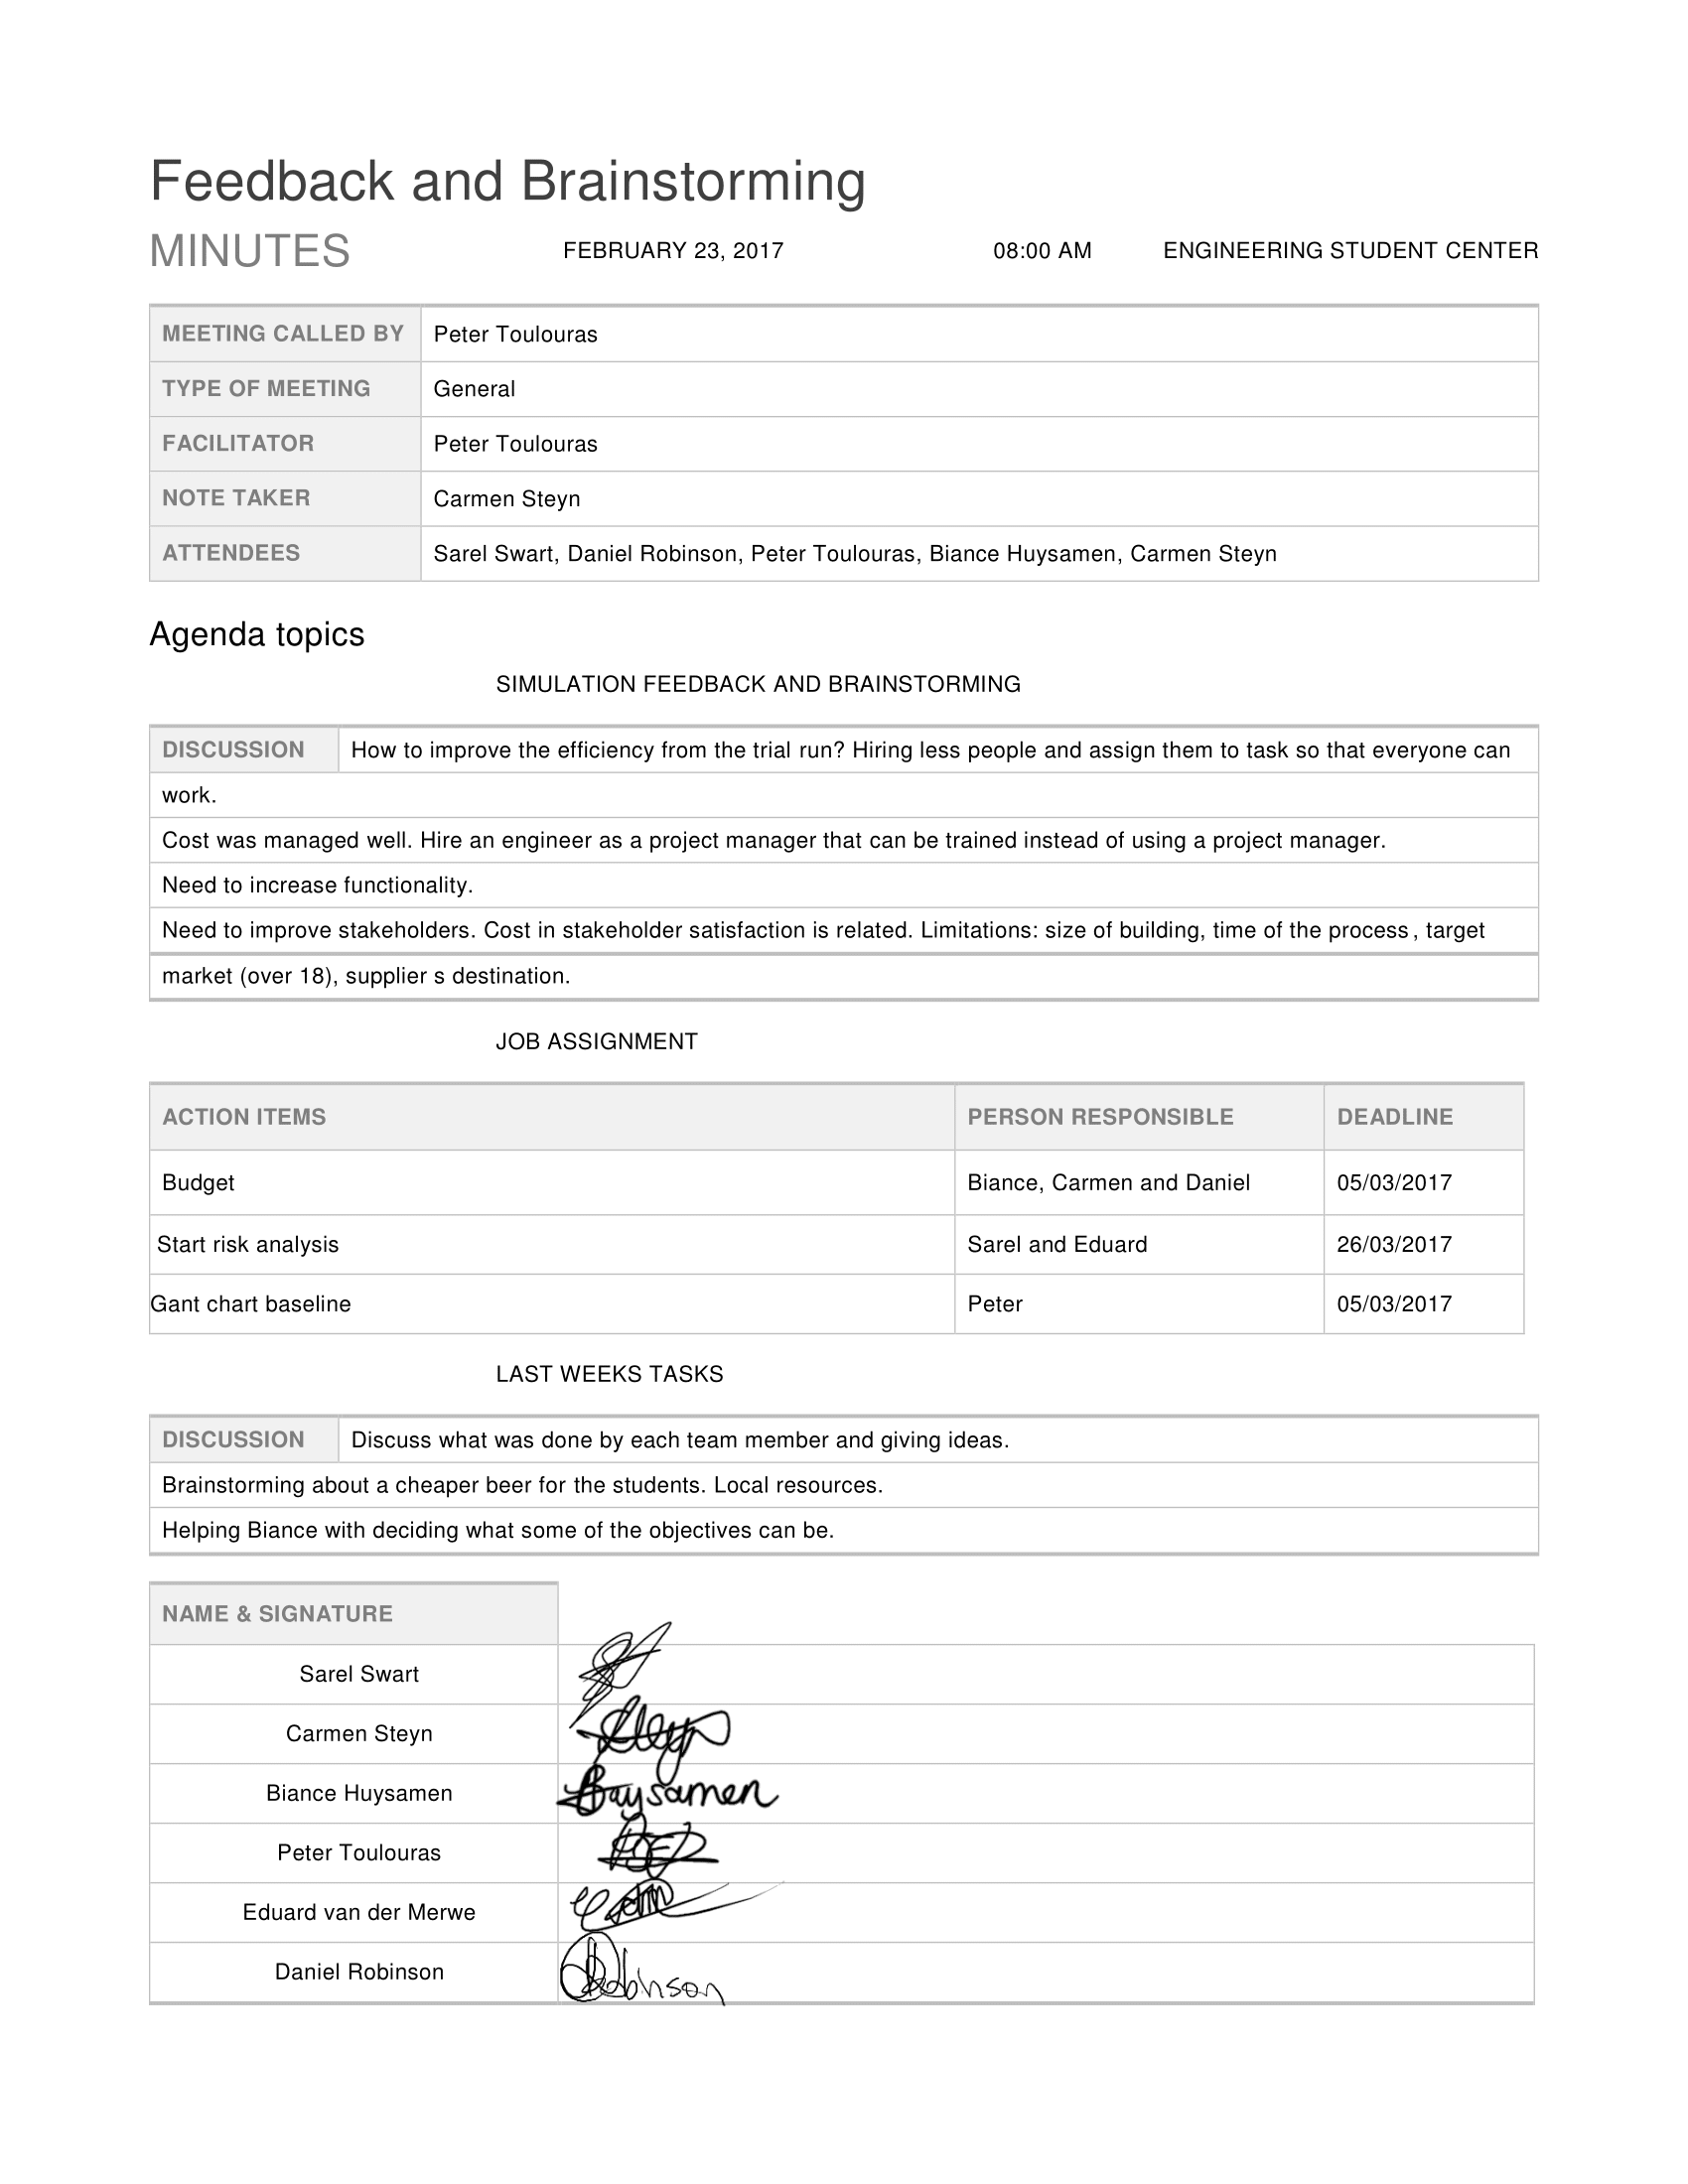
\includegraphics[scale=0.25]{Meeting_minutes_23_Feb.png}
\caption{Minutes 23 Feb}
\end{figure}

\begin{figure}[H]
\centering
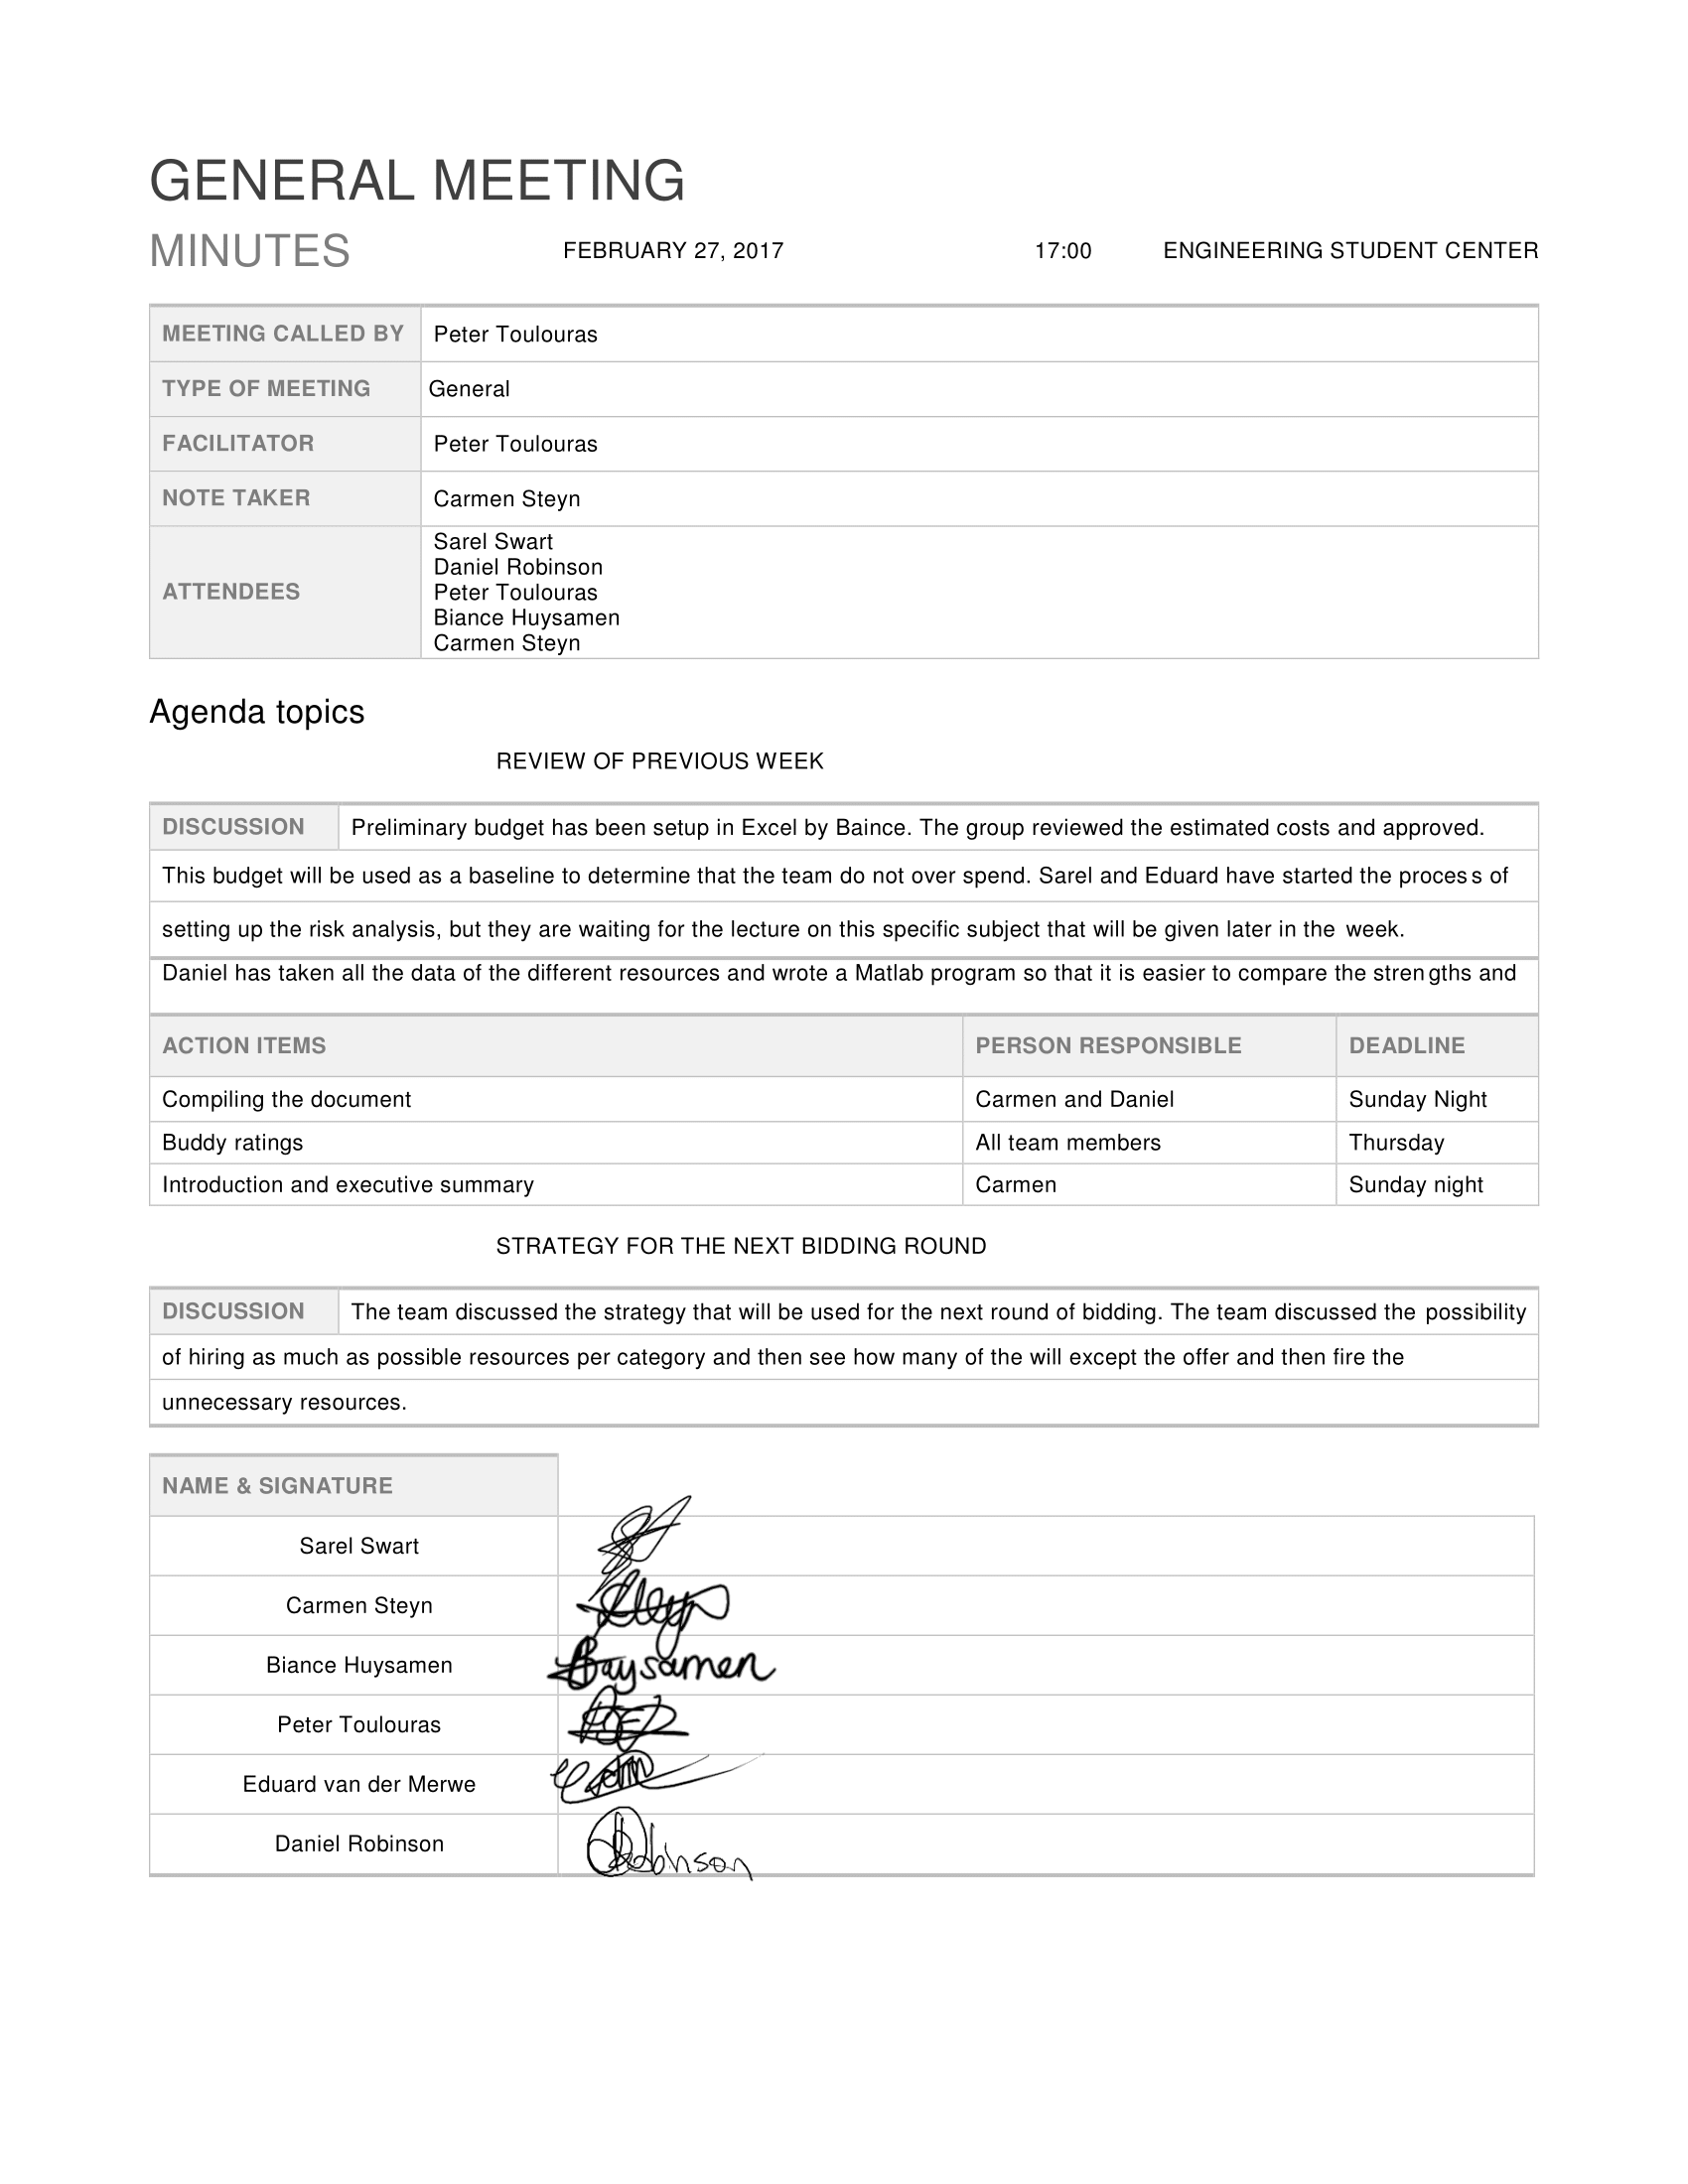
\includegraphics[scale=0.25]{Meeting_minutes_27_Feb.png}
\caption{Minutes 27 Feb}
\end{figure}

\begin{figure}[H]
\centering
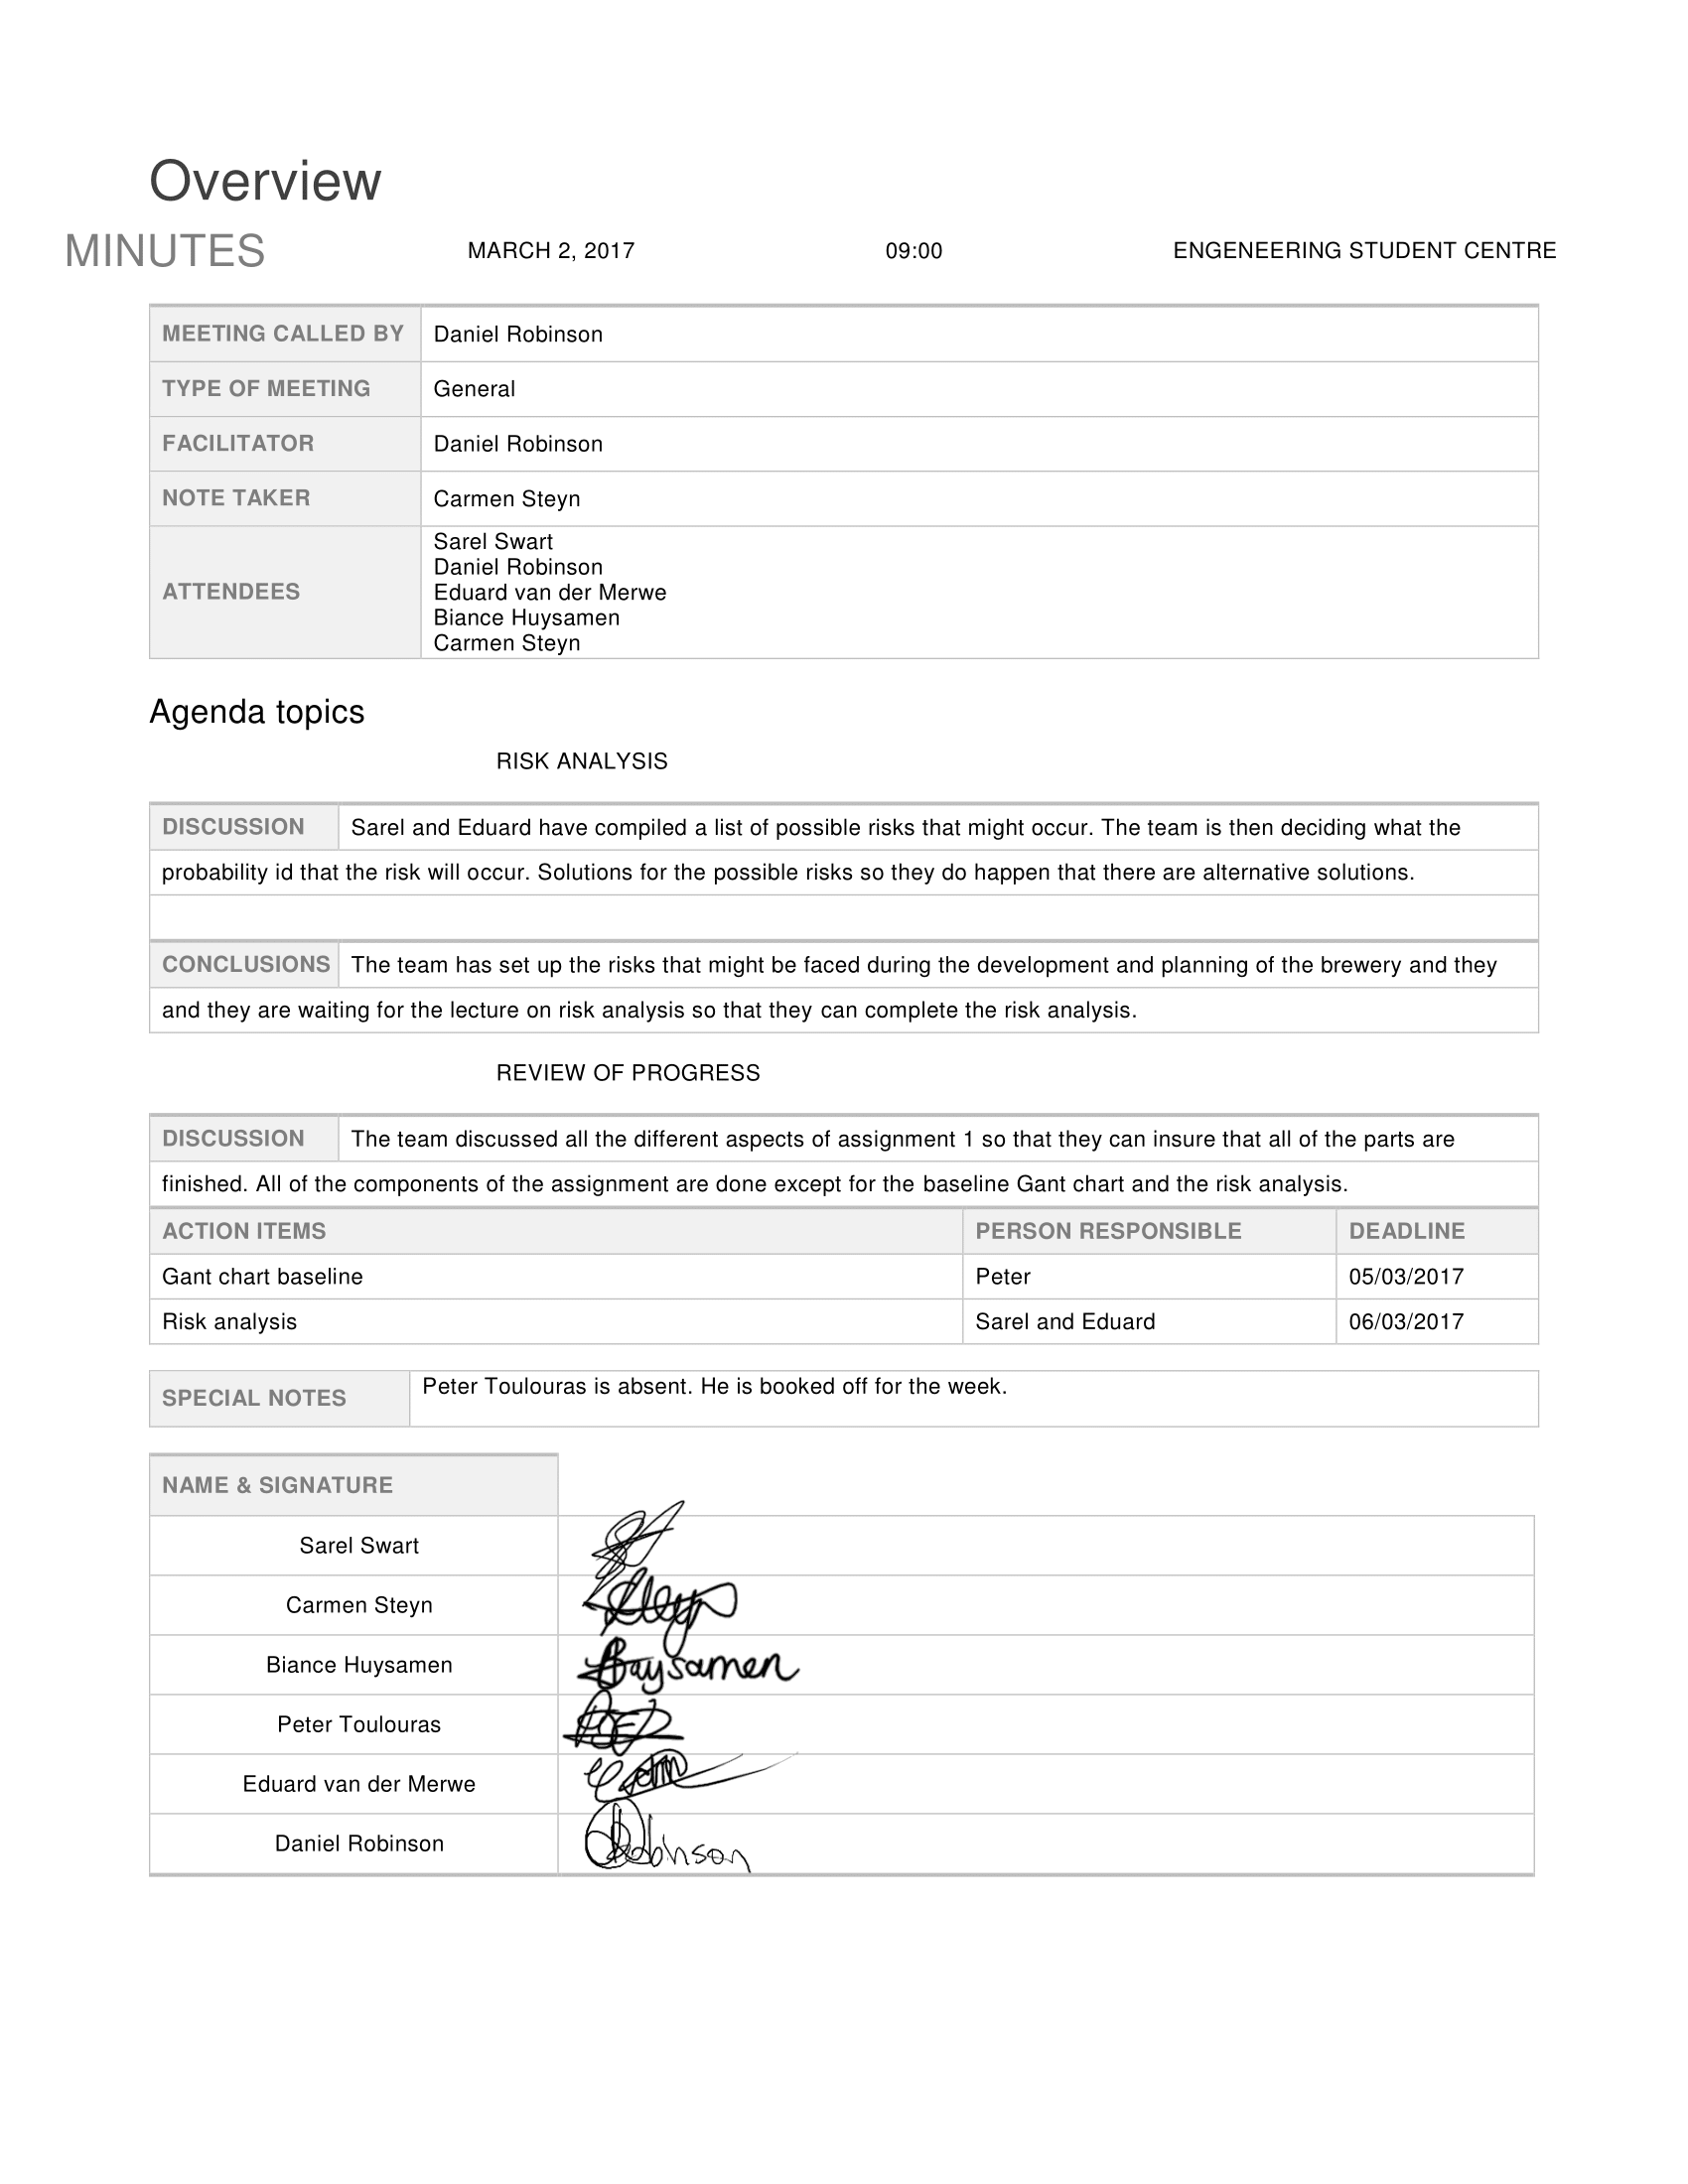
\includegraphics[scale=0.25]{Meeting_minutes_02_March.png}
\caption{Minutes 2 March}
\end{figure}

\begin{figure}[H]
\centering
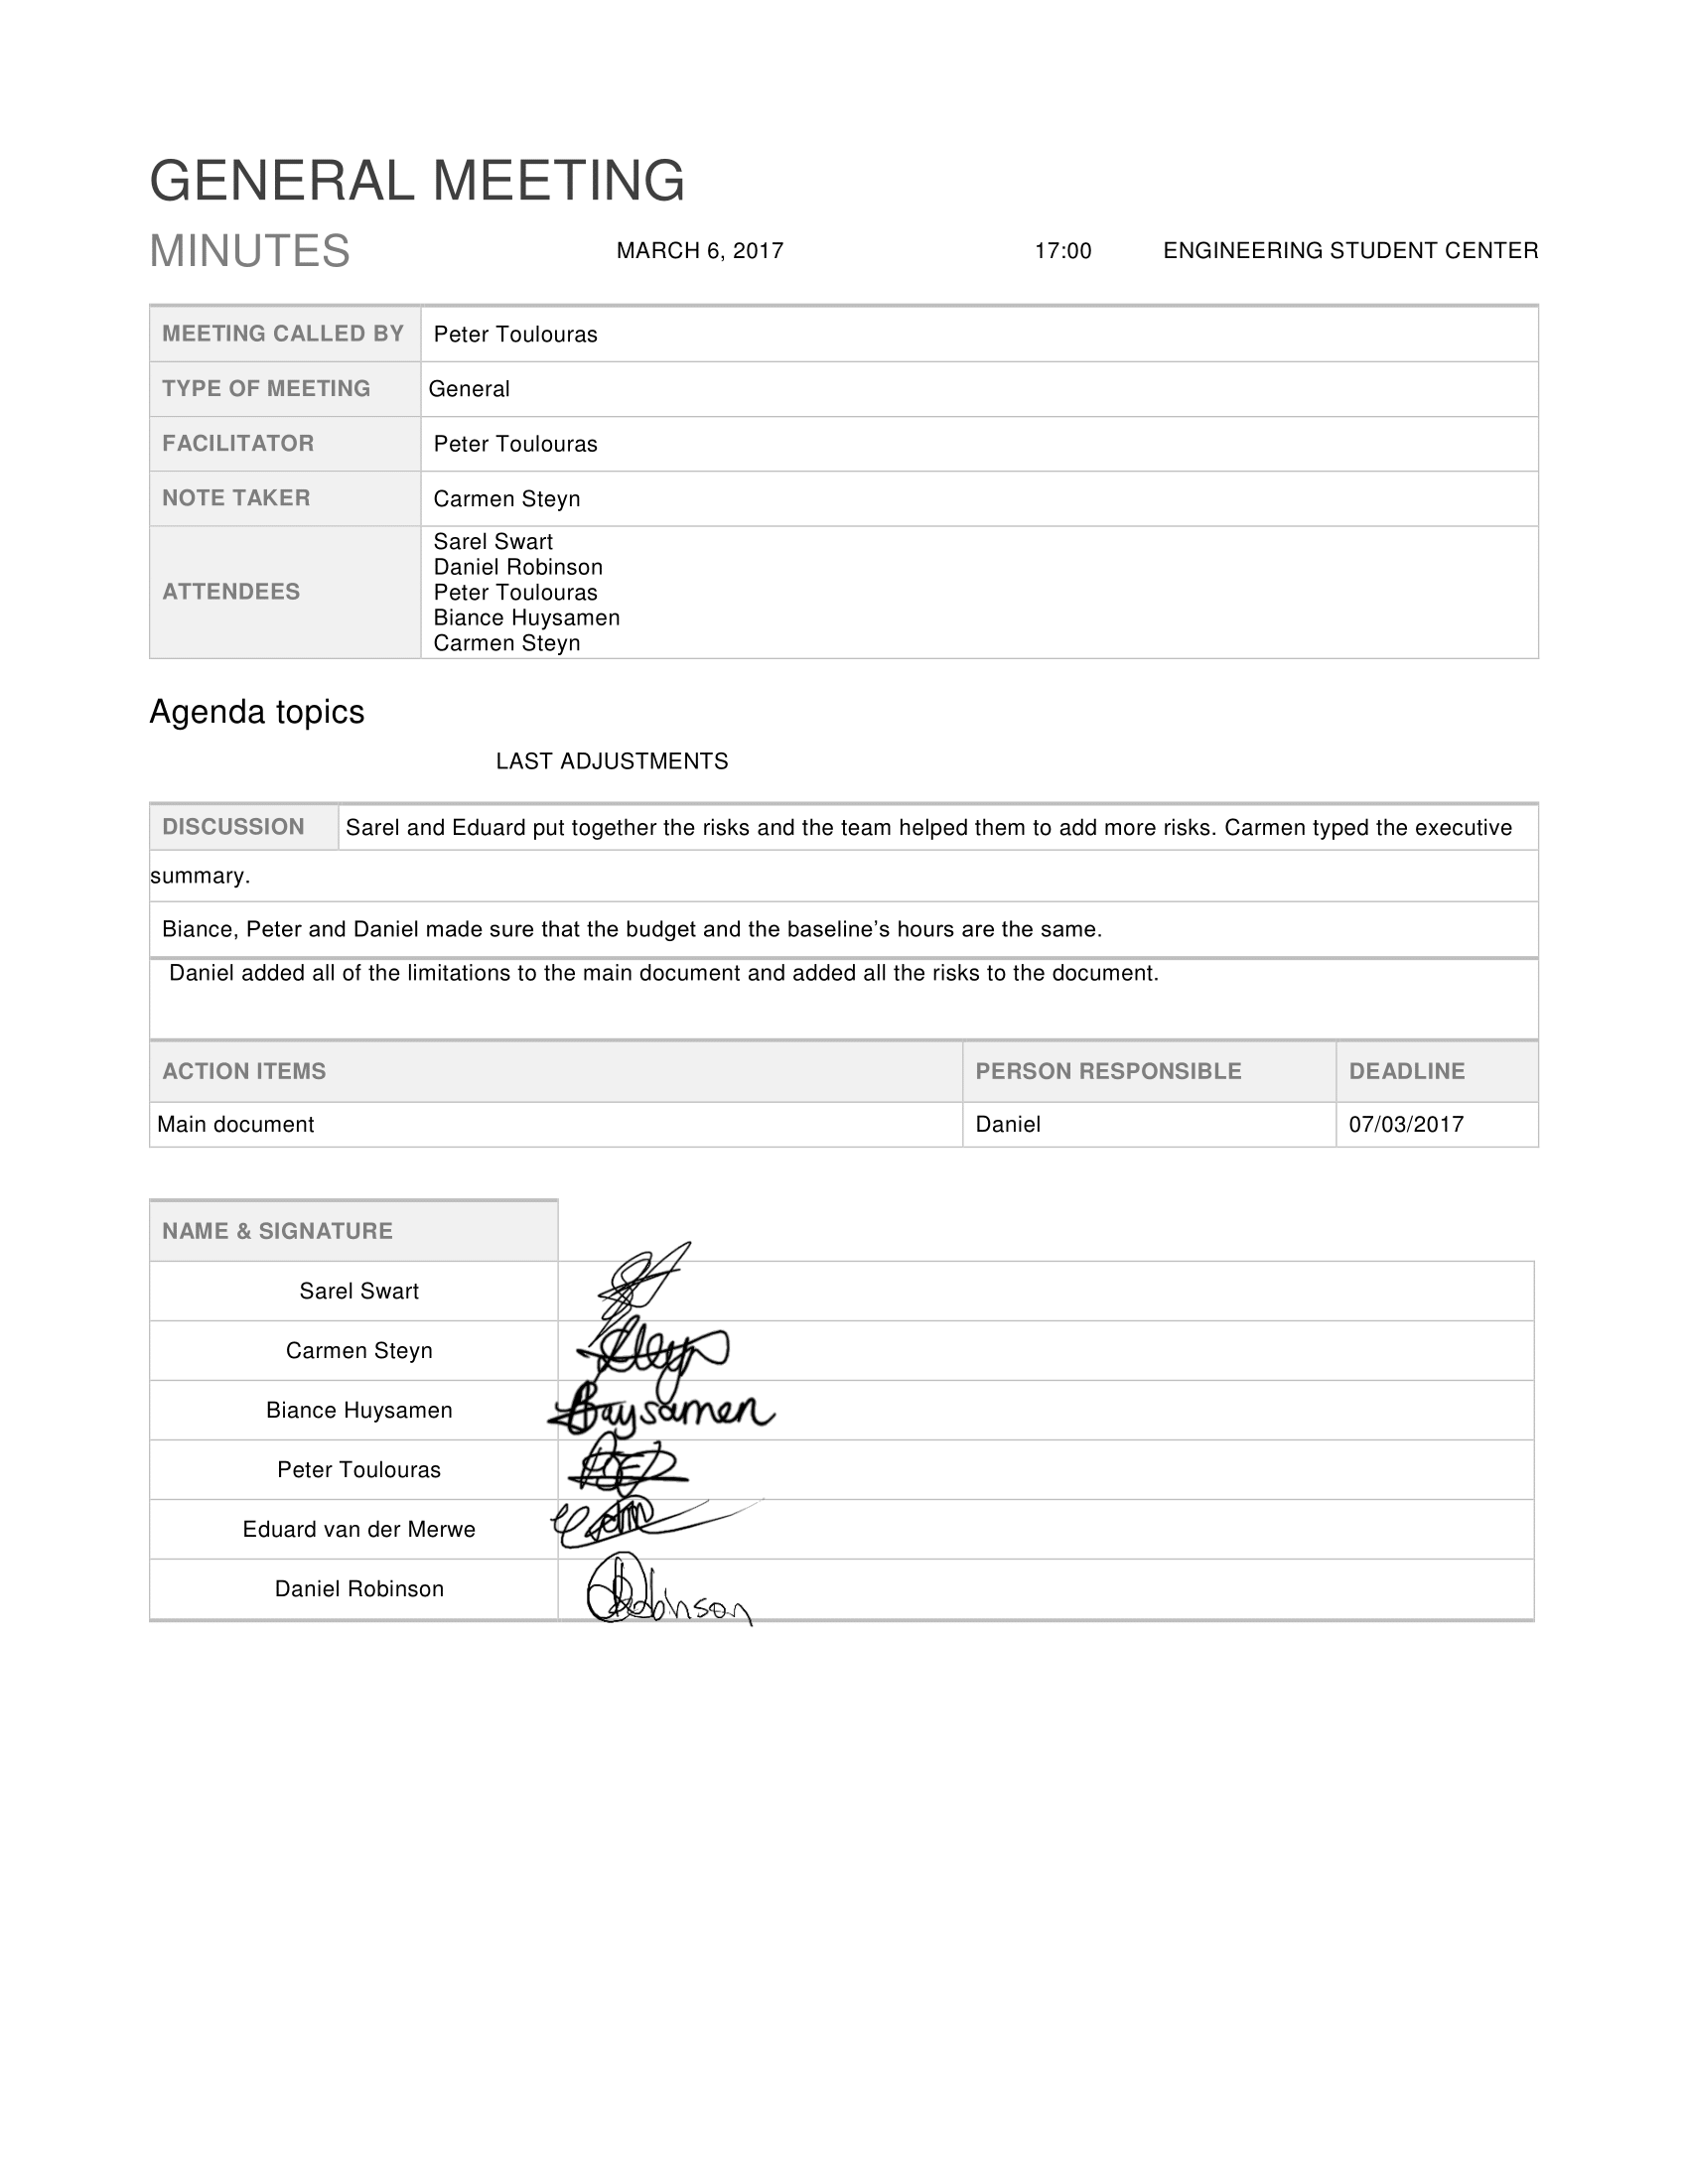
\includegraphics[scale=0.25]{Meeting_minutes_6_March.png}
\caption{Minutes 6 March}
\end{figure}

\end{appendices}

\newpage
\section*{References}

Anon., n.d. Stellenbrau. [Online] 
Available at: http://stellenbrau.co.za/pages/our-beers.php
[Accessed 20 02 2017].\\\\

\noindent
M.Nicholas, J. \& Steyn, H., 2008. Project Managment for Engineering. In: Business and Technology. New York: Routledge, pp. 43, 347.



\bibliographystyle{plain}
% \bibliographystyle{alpha}
\bibliography{references}

\end{document}


% \begin{figure}[H]
% \begin{subfigure}{0.5\textwidth}
% 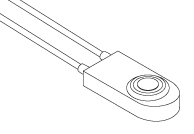
\includegraphics[scale=0.3]{3.png}
% \caption{Pushbutton Switch.\\
% Reproduced from \cite{cpi}.}
% \label{fig:p}
% \end{subfigure}
% \begin{subfigure}{0.5\textwidth}
% \centering
% 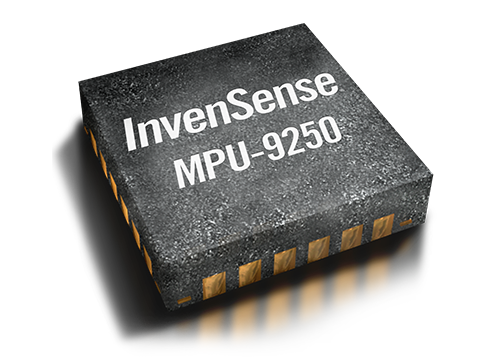
\includegraphics[scale=0.1]{2.png}
% \caption{InvenSense MPU-9250.\\
% Reproduced from\cite{iven}.}
% \label{fig:att}
% \end{subfigure}
% \begin{subfigure}{0.5\textwidth}
% \centering
% 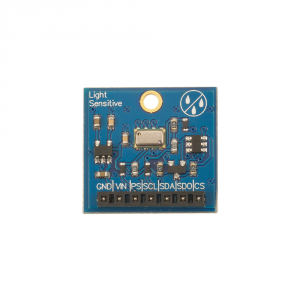
\includegraphics[scale=0.3]{1.png}
% \caption{Altimeter Module MS5607.\\ Reproduced from \cite{par}.}
% \label{fig:pres}
% \end{subfigure}
% \caption{Sensors}
% \label{fig:sensors}
% \end{figure}


% In order for the data to be transmitted successfully, it needs to be in a format acceptable by the GCS. The data will be stored in a JSON packet created using a C++ library\cite{ajson}.

% Code block \ref{code:json1} shows a potential data packet.

% \lstset{language=html,caption={Potential packet},label=code:json1}
% \begin{lstlisting}
% {
%   "temperature": "11.3",
%   "pressure": "99.325"
% }
% \end{lstlisting}

% \begin{figure}
% \centering
% 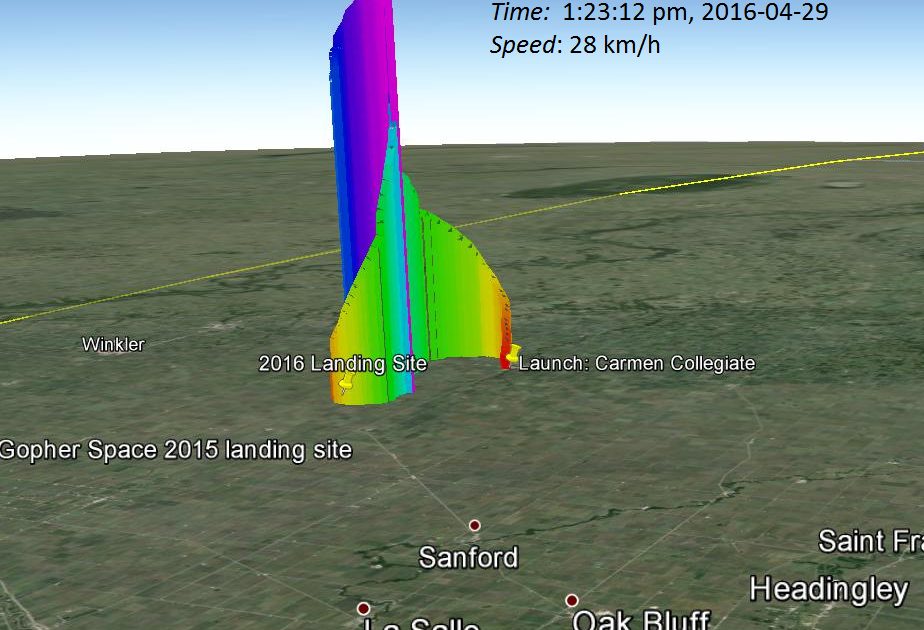
\includegraphics[scale=0.35]{flight_path.png}
% \caption{CanSat flight trajectory\\
% Reproduced from \cite{gopher}}
% \label{fig:flight_path}
% \end{figure}




% \subsection{How to add Tables}

% Use the table and tabular commands for basic tables --- see Table~\ref{tab:widgets}, for example. 

% \begin{table}
% \centering
% \begin{tabular}{l|r}
% Item & Quantity \\\hline
% Widgets & 42 \\
% Gadgets & 13
% \end{tabular}
% \caption{\label{tab:widgets}An example table.}
% \end{table}

% \subsection{How to write Mathematics}

% \LaTeX{} is great at typesetting mathematics. Let $X_1, X_2, \ldots, X_n$ be a sequence of independent and identically distributed random variables with $\text{E}[X_i] = \mu$ and $\text{Var}[X_i] = \sigma^2 < \infty$, and let
% \[S_n = \frac{X_1 + X_2 + \cdots + X_n}{n}
%       = \frac{1}{n}\sum_{i}^{n} X_i\]
% denote their mean. Then as $n$ approaches infinity, the random variables $\sqrt{n}(S_n - \mu)$ converge in distribution to a normal $\mathcal{N}(0, \sigma^2)$.


% \subsection{How to create Sections and Subsections}

% Use section and subsections to organize your document. Simply use the section and subsection buttons in the toolbar to create them, and we'll handle all the formatting and numbering automatically.

% \subsection{How to add Lists}

% You can make lists with automatic numbering \dots

% \begin{enumerate}
% \item Like this,
% \item and like this.
% \end{enumerate}
% \dots or bullet points \dots
% \begin{itemize}
% \item Like this,
% \item and like this.
% \end{itemize}

% \subsection{How to add Citations and a References List}

% You can upload a \verb|.bib| file containing your BibTeX entries, created with JabRef; or import your \href{https://www.overleaf.com/blog/184}{Mendeley}, CiteULike or Zotero library as a \verb|.bib| file. You can then cite entries from it, like this: \cite{greenwade93}. Just remember to specify a bibliography style, as well as the filename of the \verb|.bib|.

% You can find a \href{https://www.overleaf.com/help/97-how-to-include-a-bibliography-using-bibtex}{video tutorial here} to learn more about BibTeX.

% We hope you find Overleaf useful, and please let us know if you have any feedback using the help menu above --- or use the contact form at \url{https://www.overleaf.com/contact}!

%\newpage
%\bibliographystyle{plain}
%% \bibliographystyle{alpha}
%\bibliography{references}